
\section{introduction: correctness}
\usetikzlibrary{arrows.meta}
% not fragile to prevent .vrb from referring to wrong thing
\begin{frame}<0>[label=pthreadCreateBrokenP]{a threading race}
\vspace{-.25cm}
\lstinputlisting[
    style=small,
    language=C++,
    moredelim={**[is][\btHL<1|handout:1>]{@1}{1@}},
]{../threads/pthread-create-race-code.c}
My machine: outputs \texttt{In the thread} \myemph{about 4\% of the time}. \\
What happened?
\end{frame}


\begin{frame}<0>[label=pthreadCreateRace]{a race}
\begin{itemize}
\item returning from main \myemph{exits the entire process} (all its threads)
    \begin{itemize}
    \item same as calling exit; not like other threads
    \end{itemize}
\item race: main's return 0 or print\_message's printf first?
\end{itemize}
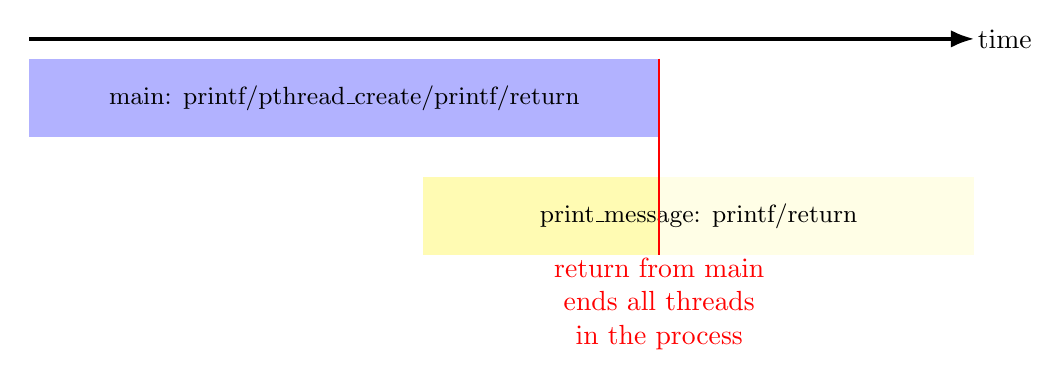
\begin{tikzpicture}
\tikzset{
    box/.style={draw,thick},
    main box/.style={fill=blue!30},
    thread box/.style={fill=yellow!30},
    my label/.style={font=\small},
    >=Latex,
}
\draw[very thick,->] (0,1.25) -- (12,1.25) node[right] {time};
\path[main box] (0, 0) rectangle (8, 1) node[midway,my label]{main: printf/pthread\_create/printf/return};
\path[thread box] (5, -.5) rectangle (8, -1.5);
\path[thread box,fill=yellow!10,dashed] (8, -.5) rectangle (12, -1.5);
\path (5, -.5) rectangle (12, -1.5) node[midway,my label]{print\_message: printf/return};
\path[draw,thick,red] (8, 1) -- (8,-1.5) node[below,align=center] {return from main \\ ends all threads \\ in the process};
\end{tikzpicture}
\end{frame}


\againframe<1>{pthreadCreateBrokenP}

\againframe<1>{pthreadCreateRace}
\begin{frame}{the correctness problem}
\begin{itemize}
\item two threads?
\item introduces \textit{non-determinism}
\item which one runs first?
\vspace{.5cm}
\item allows for ``race condition'' bugs
\item \ldots to be avoided with synchronization constructs
\end{itemize}
\end{frame}


\section{the lost write}

\subsection{motivation: threaded ATM server?}
\usetikzlibrary{fit}
% 

\begin{frame}{example application: ATM server}
\begin{itemize}
    \item commands: withdraw, deposit
    \item one correctness goal: don't lose money
\end{itemize}
\end{frame}

\begin{frame}[fragile,label=serverCode]{ATM server}
\vspace{-.5cm}
{\small (pseudocode)}
\begin{lstlisting}[language=C++,style=small]
ServerLoop() {
    while (true) {
        ReceiveRequest(&operation, &accountNumber, &amount);
        if (operation == DEPOSIT) {
            Deposit(accountNumber, amount);
        } else ...
    }
}
Deposit(accountNumber, amount) {
    account = GetAccount(accountNumber);
    account->balance += amount;
    SaveAccountUpdates(account);
}
\end{lstlisting}
\end{frame}

\begin{frame}[fragile,label=threadedServerWhy]{a threaded server?}
\begin{lstlisting}[
    language=C++,
    style=small,
    moredelim={**[is][\btHL<1-|handout:1->]{@1}{1@}}
]
Deposit(accountNumber, amount) {
    account = @1GetAccount(accountId)1@;
    account->balance += amount;
    @1SaveAccountUpdates(account);1@
}
\end{lstlisting}
\begin{itemize}
\item maybe GetAccount/SaveAccountUpdates can be slow?
    \begin{itemize}
    \item read/write disk sometimes? contact another server sometimes?
    \end{itemize}
\item maybe lots of requests to process?
    \begin{itemize}
    \item maybe real logic has more checks than Deposit()
    \item \ldots
    \end{itemize}
\item all reasons to handle multiple requests at once
\item $\rightarrow$ many threads all running the server loop
\end{itemize}
\end{frame}

\begin{frame}[fragile,label=threadedServerLoop]{multiple threads}
\begin{lstlisting}[
    language=C++,
    style=smaller,
    moredelim={**[is][\btHL<1-|handout:1->]{@1}{1@}}
]
main() {
    for (int i = 0; i < NumberOfThreads; ++i) {
        pthread_create(&server_loop_threads[i], NULL,
                       ServerLoop, NULL);
    }
    ...
}

ServerLoop() {
    while (true) {
        ReceiveRequest(&operation, &accountNumber, &amount);
        if (operation == DEPOSIT) {
            Deposit(accountNumber, amount);
        } else ...
    }
}
\end{lstlisting}
\end{frame}


\subsection{example}
\begin{frame}[fragile,label=theLostWrite]{the lost write}
\begin{tikzpicture}
\node (cpp code) {
\begin{lstlisting}[language=C++,style=small]
account->balance += amount;
\end{lstlisting}
};
    \node[anchor=west] at (cpp code.east) { (in two threads, same account) };
    \draw[very thick,dotted] (cpp code.south west) -- ++(15cm,0cm);

\node[label={north:Thread A},align=left,anchor=north west] (thread A part 1) at ([yshift=-1cm]cpp code.south west) {
\begin{lstlisting}[language=myasm,style=small]
mov account->balance, %rax
add amount, %rax
\end{lstlisting}
};
\node[label={north:Thread B},anchor=north west] (thread B top) at ([xshift=.5cm]thread A part 1.north east) {
\hspace{5cm}
};
\node[align=left,anchor=north west] (thread B part 1) at (thread B top.west |- thread A part 1.south) {
\begin{lstlisting}[language=myasm,style=small]
mov account->balance, %rax
add amount, %rax
\end{lstlisting}
};
\node[align=left,anchor=north west] (thread A part 2) at (thread A part 1.west |- thread B part 1.south) {
\begin{lstlisting}[language=myasm,style=small]
mov %rax, account->balance
\end{lstlisting}
};
\node[align=left,anchor=north west] (thread B part 2) at (thread B part 1.west |- thread A part 2.south) {
\begin{lstlisting}[language=myasm,style=small]
mov %rax, account->balance
\end{lstlisting}
};
\foreach \place in {thread A part 1,thread B part 1,thread A part 2} {
    \draw[ultra thick] (\place.south -| thread A part 1.west) -- (\place.south -| thread B part 1.east)
        node[midway,fill=white,font=\small]{context switch};
}
\begin{visibleenv}<2->
    \node[draw,red,ultra thick,fit=(thread A part 2),
        label={[red]south:lost write to balance}] {};
    \node[draw,blue,ultra thick,fit=(thread B part 2),
        label={[blue]south:``winner'' of the race}] {};
\end{visibleenv}
\begin{visibleenv}<3->
    \node[draw,red,ultra thick,anchor=north] at ([yshift=-1cm]thread B part 2.south west) {
        lost track of thread A's money
    };
\end{visibleenv}
\end{tikzpicture}
\end{frame}


\section{race conditions and atomicity}
\subsection{thinking about simple races} 
\begin{frame}{thinking about race conditions (1)}
\begin{itemize}
\item what are the possible values of $x$? \\
\item (initially $x = y = 0$) \\
\begin{tabular}{cc}
    \bfseries{Thread A} & \bfseries{Thread B} \\ \hline
    $x \leftarrow 1$ & $y \leftarrow 2$ \\
\end{tabular}
\iftoggle{heldback}{}{
\item<2-> must be 1. Thread B can't do anything
}
\end{itemize}
\end{frame}

\begin{frame}<1-2>[label=thinkRace2]{thinking about race conditions (2)}
\begin{itemize}
\item what are some possible values of $x$? \\
\item (initially $x = y = 0$) \\
\begin{tabular}{cc}
    \bfseries{Thread A} & \bfseries{Thread B} \\ \hline
    $x \leftarrow y + 1$ & $y \leftarrow 2$ \\
                    ~ & $y \leftarrow y \times 2$ \\
\end{tabular}
\iftoggle{heldback}{}{
\item<2-> if A goes first, then B: $1$
\item<2-> if B goes first, then A: $5$
\item<2-> if B line one, then A, then B line two: $3$
\item<3-> \ldots and why not 7:
    \begin{itemize}
    \item B (start): $y \leftarrow 2 = 0010_{\text{TWO}}$; then y bit 3 $\leftarrow$ 0; y bit 2 $\leftarrow$ 1; then
    \item A: x $\leftarrow 110_{\text{TWO}} + 1 = 7$; then
    \item B (finish): y bit 1 $\leftarrow$ 0; y bit 0 $\leftarrow$ 0
    \end{itemize}
}
\end{itemize}
\end{frame}

\begin{frame}{thinking about race conditions (3)}
\begin{itemize}
\item what are the possible values of $x$? \\
\item (initially $x = y = 0$) \\
\begin{tabular}{cc}
    \bfseries{Thread A} & \bfseries{Thread B} \\ \hline
    $x \leftarrow 1$ & $x \leftarrow 2$ \\
\end{tabular}
\iftoggle{heldback}{}{
\item<2-> 1 or 2
\item<3-> \ldots but why not 3?
    \begin{itemize}
    \item B: x bit 0 $\leftarrow 0$
    \item A: x bit 0 $\leftarrow 1$
    \item A: x bit 1 $\leftarrow 0$
    \item B: x bit 1 $\leftarrow 1$
    \end{itemize}
}
\end{itemize}
\end{frame}

\againframe<3>{thinkRace2}


\subsection{atomicity definition}
\begin{frame}{atomic operation}
\begin{itemize}
\item \textit{atomic operation} = operation that runs to completion or not at all
\item we will use these to let threads work together
\vspace{.5cm}
\item most machines: loading/storing {\small (aligned)} words is atomic
    \begin{itemize}
    \item so can't get $3$ from $x \leftarrow 1$ and $x \leftarrow 2$ running in parallel
    \item aligned $\approx$ address of word is multiple of word size (typically done by compilers)
    \end{itemize}
\item but some instructions are not atomic; examples:
    \begin{itemize}
    \item x86: integer \texttt{add} constant to memory location
    \item many CPUs: loading/storing values that cross cache blocks
        \begin{itemize}
            \item e.g. if cache blocks \texttt{0x40} bytes, load/store 4 byte from addr. \texttt{0x3E} is not atomic
        \end{itemize}
    \end{itemize}
\end{itemize}
\end{frame}



\subsection{example: x86 add not atomic}

\begin{frame}[fragile,label=lostAdds]{lost adds (program)}
\begin{lstlisting}[language=myasm,style=smaller]
.global update_loop
update_loop:
    addl $1, the_value // the_value (global variable) += 1
    dec %rdi           // argument 1 -= 1
    jg update_loop     // if argument 1 >= 0 repeat
    ret
\end{lstlisting}
\hrule
\begin{lstlisting}[language=C++,style=smaller]
int the_value;
extern void *update_loop(void *);
int main(void) {
    the_value = 0;
    pthread_t A, B;
    pthread_create(&A, NULL, update_loop, (void*) 1000000);
    pthread_create(&B, NULL, update_loop, (void*) 1000000);
    pthread_join(A, NULL); pthread_join(B, NULL);
    // expected result: 1000000 + 1000000 = 2000000
    printf("the_value = %d\n", the_value);
}
\end{lstlisting}
\end{frame}

\begin{frame}[fragile,label=lostAddsResult]{lost adds (results)}
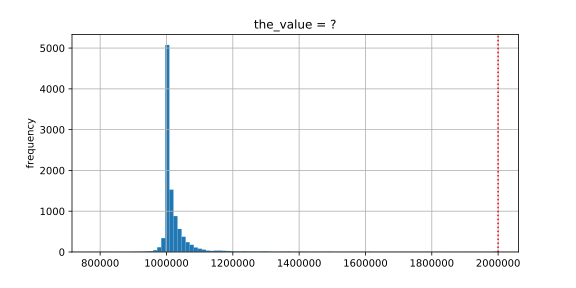
\includegraphics[width=1.1\textwidth]{../sync/parallel-add-histogram}
\end{frame}

\begin{frame}{but how?}
    \begin{itemize}
    \item probably not possible on single core
        \begin{itemize}
            \item exceptions can't occur in the middle of \texttt{add} instruction
        \end{itemize}
    \item \ldots but `add to memory' implemented with multiple steps
        \begin{itemize}
        \item still needs to load, add, store internally
        \item can be interleaved with what other cores do
        \end{itemize}
        \vspace{.5cm}
    \item<2-> {\small (and actually it's more complicated than that --- we'll talk later)}
    \end{itemize}
\end{frame}



\subsection{what is atomic?}

\begin{frame}{so, what is actually atomic}
    \begin{itemize}
    \item for now we'll assume: load/stores of `words' 
        \begin{itemize}
        \item  (64-bit machine = 64-bits words)
        \end{itemize}
        \vspace{.5cm}
    \item in general: \myemph{processor designer will tell you}
    \item their job to design caches, etc. to work as documented
    \end{itemize}
\end{frame}


\section{too much milk: locks from load/store?}

\subsection{setup: buying milk}
\begin{frame}{too much milk}
\begin{itemize}
\item roommates Alice and Bob want to keep fridge stocked with milk:
\end{itemize}
\begin{tabular}{l|l|l}
    time & Alice & Bob \\ \hline\hline
    3:00 & look in fridge. no milk & ~\\ \hline
    3:05 & leave for store & ~\\ \hline
    3:10 & arrive at store & look in fridge. no milk \\ \hline
    3:15 & buy milk & leave for store \\ \hline
    3:20 & return home, put milk in fridge & arrive at store \\ \hline
    3:25 & ~ & buy milk \\ \hline
    3:30 & ~ & return home, put milk in fridge\\ \hline
\end{tabular}
\\
how can Alice and Bob coordinate better?
\end{frame}




\subsection{wrong solution 1: missed notes}
\usetikzlibrary{arrows.meta}
\begin{frame}[fragile,label=solutionOne]{too much milk ``solution'' 1 (algorithm)}
\begin{itemize}
\item leave a note: ``I am buying milk''
    \begin{itemize}
    \item place before buying
    \item remove after buying
    \item don't try buying if there's a note
    \end{itemize}
\item $\approx$ setting/checking a variable (e.g. ``\texttt{note = 1}'')
\begin{itemize}\item with atomic load/store of variable\end{itemize}
\end{itemize}
\begin{lstlisting}[language=C++,style=small]
if (no milk) {
    if (no note) {
        leave note;
        buy milk;
        remove note;
    }
}
\end{lstlisting}
\begin{itemize}
\item<2-> \myemph{exercise: why doesn't this work?}
\end{itemize}
\end{frame}

\begin{frame}[fragile,label=solutionOneTimeline]{too much milk ``solution'' 1 (timeline)}
\begin{tikzpicture}
\tikzset{
    every label/.style={font=\bfseries},
    every node/.style={inner sep=0.5mm},
}
\node[label={north:Alice},align=left,anchor=north west] (thread A part 1) {
\begin{lstlisting}[language=C++,style=small]
if (no milk) {
    if (no note) {
\end{lstlisting}
};
\node[label={north:Bob},anchor=north west] (thread B top) at ([xshift=2cm]thread A part 1.north east) {
\hspace{5cm}
};
\node[align=left,anchor=north west] (thread B part 1) at (thread B top.west |- thread A part 1.south) {
\begin{lstlisting}[language=C++,style=small]
if (no milk) {
    if (no note) {
\end{lstlisting}
};
\node[align=left,anchor=north west] (thread A part 2) at (thread A part 1.west |- thread B part 1.south) {
\begin{lstlisting}[language=C++,style=small]
        leave note;
        buy milk;
        remove note;
    }
}
\end{lstlisting}
};
\node[align=left,anchor=north west] (thread B part 2) at (thread B part 1.west |- thread A part 2.south) {
\begin{lstlisting}[language=C++,style=small]
        leave note;
        buy milk;
        remove note;
    }
}
\end{lstlisting}
};
\end{tikzpicture}
\end{frame}



\subsection{wrong solution 2: read own note}
\begin{frame}[fragile,label=solutionTwo]{too much milk ``solution'' 2 (algorithm)}
\begin{itemize}
\item intuition: leave note when buying \myemph{or checking if need to buy}
\end{itemize}
\begin{lstlisting}[language=C++,style=small]
leave note;
if (no milk) {
    if (no note) {
        buy milk;
    }
}
remove note;
\end{lstlisting}
\end{frame}

\begin{frame}[fragile,label=solutionTwoTimeline]{too much milk: ``solution'' 2 (timeline)}
\begin{tikzpicture}
\tikzset{
    >=Latex,
}
\begin{scope}
\tikzset{
    every label/.style={font=\bfseries},
    every node/.style={inner sep=0.25mm},
}
\node[label={north:Alice},align=left,anchor=north west] (thread A part 1) {
\begin{lstlisting}[language=C++,style=small,moredelim={**[is][\btHL<2-|handout:2->]{@2}{2@}}]
leave note;
if (no milk) {
    if (@2no note2@) {
\end{lstlisting}
};
\node[anchor=north west] (thread A part 2) at (thread A part 1.south west) {
\begin{lstlisting}[language=C++,style=small,moredelim={**[is][\btHL<1-|handout:1->]{@2}{2@}}]
        buy milk;
\end{lstlisting}
};
\node[anchor=north west] (thread A part 3) at (thread A part 2.south west) {
\begin{lstlisting}[language=C++,style=small,moredelim={**[is][\btHL<1-|handout:1->]{@2}{2@}}]
    }
}
remove note;
\end{lstlisting}
};
\end{scope}
\begin{visibleenv}<2->
    \draw[black,very thick,<-] ([yshift=3mm]thread A part 1.south east) -- ++(1cm, 0cm) node[right] (always a note) {
        but there's \myemph{always a note}
    };
\end{visibleenv}
\begin{visibleenv}<3->
    \draw[ultra thick,black] ([xshift=2cm]thread A part 2.south west) -- (thread A part 2.north east);
    \node[anchor=north west] at (always a note.south west) {
        \ldots will never buy milk (twice \textit{or} once)
    };
\end{visibleenv}
\end{tikzpicture}
\end{frame}



\subsection{wrong solution 3: too little milk}
\begin{frame}[fragile,label=solutionThree]{``solution'' 3: algorithm}
\begin{itemize}
\item intuition: label notes so Alice knows which is hers (and vice-versa)
    \begin{itemize}
    \item computer equivalent: separate noteFromAlice and noteFromBob variables
    \end{itemize}
\end{itemize}
\begin{tikzpicture}
\tikzset{
    >=Latex,
}
\begin{scope}
\tikzset{
    every label/.style={font=\bfseries},
    every node/.style={inner sep=0.25mm},
}
\node[label={north:Alice},align=left,anchor=north west] (thread A part 1) {
\begin{lstlisting}[language=C++,style=small,moredelim={**[is][\btHL<2-|handout:2->]{@2}{2@}}]
leave note from Alice;
if (no milk) {
    if (no note from Bob) {
        buy milk
    }
}
remove note from Alice;
\end{lstlisting}
};
\node[label={north:Bob},anchor=north west] (thread B part 1) at ([xshift=2cm]thread A part 1.north east) {
\begin{lstlisting}[language=C++,style=small,moredelim={**[is][\btHL<2-|handout:2->]{@2}{2@}}]
leave note from Bob;
if (no milk) {
    if (no note from Alice) {
        buy milk
    }
}
remove note from Bob;
\end{lstlisting}
};
\end{scope}
\end{tikzpicture}
\end{frame}

\begin{frame}[fragile,label=solutionThreeTimeline]{too much milk: ``solution'' 3 (timeline)}
\begin{tikzpicture}
\tikzset{
    >=Latex,
}
\begin{scope}
\tikzset{
    every label/.style={font=\bfseries},
    every node/.style={inner sep=0.25mm},
}
\node[label={north:Alice},align=left,anchor=north west] (thread A part 1) {
\begin{lstlisting}[language=C++,style=small]
leave note from Alice
if (no milk) {
\end{lstlisting}
};
\node[label={north:Bob},anchor=north west] (thread B top) at ([xshift=2cm]thread A part 1.north east) {
\hspace{5cm}
};
\node[align=left,anchor=north west] (thread B part 1) at (thread B top.west |- thread A part 1.south) {
\begin{lstlisting}[language=C++,style=small]
leave note from Bob
\end{lstlisting}
};
\node[align=left,anchor=north west] (thread A part 2) at (thread A part 1.west |- thread B part 1.south) {
\begin{lstlisting}[language=C++,style=small]
    if (no note from Bob) {
        buy milk
    }
}
\end{lstlisting}
};
\node[align=left,anchor=north west] (thread B part 2) at (thread B part 1.west |- thread A part 2.south) {
\begin{lstlisting}[language=C++,style=small]
if (no milk) {
    if (no note from Alice) {
        buy milk
    }
}
remove note from Bob
\end{lstlisting}
};

\draw[ultra thick,black] ([xshift=2cm,yshift=1mm]thread A part 2.west) -- ([yshift=4mm,xshift=-2.5cm]thread A part 2.east);
\draw[ultra thick,black] ([xshift=2cm,yshift=1mm]thread B part 2.west) -- ([yshift=5mm,xshift=-3cm]thread B part 2.east);
\node[align=left,anchor=north west] (thread A part 3) at (thread A part 1.west |- thread B part 2.south) {
\begin{lstlisting}[language=C++,style=small]
remove note from Alice
\end{lstlisting}
};
\end{scope}
\end{tikzpicture}
\end{frame}


\subsection{correct solution: Peterson's algorithm}
\usetikzlibrary{arrows.meta}

\begin{frame}{too much milk: is it possible}
\begin{itemize}
\item is there a solutions with writing/reading notes?
    \begin{itemize}
    \item $\approx$ loading/storing from shared memory
    \end{itemize}
\vspace{.5cm}
\item yes, but it's not very elegant
\end{itemize}
\end{frame}

\begin{frame}[fragile,label=solutionFour]{too much milk: solution 4 (algorithm)}
\begin{tikzpicture}
\tikzset{
    >=Latex,
}
\begin{scope}
\tikzset{
    every label/.style={font=\bfseries},
    every node/.style={inner sep=0.25mm},
}
\node[label={north:Alice},align=left,anchor=north west] (thread A part 1) {
\begin{lstlisting}[language=C++,style=small,moredelim={**[is][\btHL<2-|handout:2->]{@2}{2@}}]
leave note from Alice
while (note from Bob) {
    do nothing
}
if (no milk) {
    buy milk
}
remove note from Alice
\end{lstlisting}
};
\node[label={north:Bob},anchor=north west] (thread B part 1) at ([xshift=2cm]thread A part 1.north east) {
\begin{lstlisting}[language=C++,style=small,moredelim={**[is][\btHL<2-|handout:2->]{@2}{2@}}]
leave note from Bob
if (no note from Alice) {
    if (no milk) {
        buy milk
    }
}
remove note from Bob
\end{lstlisting}
};
\end{scope}
\end{tikzpicture}
\begin{itemize}
\item<2-> exercise (hard): prove (in)correctness
\item<4-> exercise (hard): extend to three people
\end{itemize}
\end{frame}

\begin{frame}{Peterson's algorithm}
    \begin{itemize}
        \item general version of solution
        \item see, e.g., Wikipedia
            \vspace{.5cm}
        \item we'll use special hardware support instead
    \end{itemize}
\end{frame}


\section{definitions: mutual exclusion, critical section}
\begin{frame}{some definitions}
\begin{itemize}
\item \textbf{mutual exclusion}: ensuring only one thread does a particular thing at a time
    \begin{itemize}
        \item like updating shared balance
    \end{itemize}
\item<2-> \textbf{critical section}: code that exactly one thread can execute at a time
    \begin{itemize}
        \item result of mutual exclusion
    \end{itemize}
\item<3-> \textbf{lock}: object only one thread can hold at a time
    \begin{itemize}
        \item interface for creating critical sections
    \end{itemize}
\end{itemize}
\end{frame}


\section{read-modify-write atomic operations}
\begin{frame}{atomic read-modfiy-write}
    \begin{itemize}
    \item really hard to build locks for atomic load store
        \begin{itemize}
        \item and normal load/stores aren't even atomic\ldots
        \end{itemize}
    \item \ldots so processors provide \myemph{read/modify/write} operations
        \vspace{.5cm}
    \item one instruction that\\\textit{atomically}\\reads \textit{and} modifies \textit{and} writes back a value
    \end{itemize}
\end{frame}

\subsection{x86 atomic exchange} 
\begin{frame}[fragile,label=atomicXchg]{x86 atomic exchange}
\begin{lstlisting}[language=myasm]
lock xchg (%ecx), %eax
\end{lstlisting}
\begin{itemize}
    \item atomic exchange
    \item \texttt{temp $\leftarrow$ M[ECX]}
    \item \texttt{M[ECX] $\leftarrow$ EAX}
    \item \texttt{EAX $\leftarrow$ temp}
    \item \ldots without being interrupted by other processors, etc.
\end{itemize}
\end{frame}


\begin{frame}{implementing atomic exchange}
    \begin{itemize}
    \item make sure other processors don't have cache block
    \item do read+modify+write operation
    \vspace{.5cm}
    \item recall: Modified state = ``I am the only one with a copy''
    \end{itemize}
\end{frame}



\section{locks}
\begin{frame}[fragile,label=lockDefn]{the lock primitive}
    \begin{itemize}
    \item locks: an object with (at least) two operations:
        \begin{itemize}
        \item \textit{acquire} or \textit{lock} --- wait until lock is free, then ``grab'' it
        \item \textit{release} or \textit{unlock} --- let others use lock, wakeup waiters
        \end{itemize}
    \item typical usage: everyone acquires lock before using shared resource
        \begin{itemize}
        \item forget to acquire lock? weird things happen
        \end{itemize}
    \end{itemize}
\begin{lstlisting}[language=C++,style=small]
Lock(MilkLock);
if (no milk) {
    buy milk
}
Unlock(MilkLock);
\end{lstlisting}
\end{frame}

\begin{frame}[fragile,label=pthreadMutex]{pthread mutex}
\begin{lstlisting}[language=C++,style=small]
#include <pthread.h>

pthread_mutex_t MilkLock;
pthread_mutex_init(&MilkLock, NULL);
    // or: pthread_mutex_t MilkLock =
    //              PTHREAD_MUTEX_INITIALIZER;
...
pthread_mutex_lock(&MilkLock);
if (no milk) {
    buy milk
}
pthread_mutex_unlock(&MilkLock);
\end{lstlisting}
\end{frame}


\subsection{exercise}
\begin{frame}[fragile,label=lockEx]{exercise}
    \vspace{-0.5cm}
\begin{lstlisting}[style=smaller]
pthread_mutex_t lock1 = PTHREAD_MUTEX_INITIALIZER;
pthread_mutex_t lock2 = PTHREAD_MUTEX_INITIALIZER;
string one = "init one", two = "init two";
void ThreadA() {
    pthread_mutex_lock(&lock1);
    one = "one in ThreadA";  // (A1)
    pthread_mutex_unlock(&lock1);
    pthread_mutex_lock(&lock2);
    two = "two in ThreadA";  // (A2)
    pthread_mutex_unlock(&lock2);
}
void ThreadB() {
    pthread_mutex_lock(&lock1);
    one = "one in ThreadB";  // (B1)
    pthread_mutex_lock(&lock2);
    two = "two in ThreadB";  // (B2)
    pthread_mutex_unlock(&lock2);
    pthread_mutex_unlock(&lock1);
}
\end{lstlisting}
possible values of one/two after A+B run?
\end{frame}

\begin{frame}<0>[fragile,label=lockExSln]{solution}
\begin{itemize}
\item B1+A2
    \begin{itemize}
    \item A: L(1) A1 U(1) L
    \item B: L(1) B1 L(2) B2 U(2) U(1)
    \item A: L(2) A2 U(2)
    \end{itemize}
\item NOT A1+B2
    \begin{itemize}
    \item would need to run B1 before A1 before A2 before B2
    \item not possible because Lock1 held for entire B1+B2 operation
    \item so cannot fit A1+A2 in between B1 and B2
    \end{itemize}
\end{itemize}
\end{frame}

\iftoggle{heldback}{}{\againframe<1>{lockExSln}}

\begin{frame}[fragile,label=lockExAlt1]{exercise (alternate 1)}
    \vspace{-0.5cm}
\begin{lstlisting}[style=smaller]
pthread_mutex_t lock1 = PTHREAD_MUTEX_INITIALIZER;
pthread_mutex_t lock2 = PTHREAD_MUTEX_INITIALIZER;
string one = "init one", two = "init two";
void ThreadA() {
    pthread_mutex_lock(&lock2);
    two = "two in ThreadA";  // (A2)
    pthread_mutex_unlock(&lock2);
    pthread_mutex_lock(&lock1);
    one = "one in ThreadA";  // (A1)
    pthread_mutex_unlock(&lock1);
}
void ThreadB() {
    pthread_mutex_lock(&lock1);
    one = "one in ThreadB";  // (B1)
    pthread_mutex_lock(&lock2);
    two = "two in ThreadB";  // (B2)
    pthread_mutex_unlock(&lock2);
    pthread_mutex_unlock(&lock1);
}
\end{lstlisting}
possible values of one/two after A+B run?
\end{frame}

\begin{frame}[fragile,label=lockExAlt2]{exercise (alternate 2)}
    \vspace{-0.5cm}
\begin{lstlisting}[style=smaller]
pthread_mutex_t lock1 = PTHREAD_MUTEX_INITIALIZER;
pthread_mutex_t lock2 = PTHREAD_MUTEX_INITIALIZER;
string one = "init one", two = "init two";
void ThreadA() {
    pthread_mutex_lock(&lock2);
    two = "two in ThreadA";  // (A2)
    pthread_mutex_unlock(&lock2);
    pthread_mutex_lock(&lock1);
    one = "one in ThreadA";  // (A1)
    pthread_mutex_unlock(&lock1);
}
void ThreadB() {
    pthread_mutex_lock(&lock1);
    one = "one in ThreadB";  // (B1)
    pthread_mutex_unlock(&lock1);
    pthread_mutex_lock(&lock2);
    two = "two in ThreadB";  // (B2)
    pthread_mutex_unlock(&lock2);
}
\end{lstlisting}
possible values of one/two after A+B run?
\end{frame}


\section{preview: beyond locks}
\begin{frame}{are locks enough?}
\begin{itemize}
    \item do we need more than locks?
\end{itemize}
\end{frame}

\begin{frame}{example 1: pipes?}
\begin{itemize}
\item suppose we want to implement a pipe with threads
\item \texttt{read} sometimes needs to wait for a \texttt{write}
\item don't want busy-wait
\begin{itemize}
\item (and trick of having writer unlock() so reader can finish a lock() is illegal)
\end{itemize}
\end{itemize}
\end{frame}

\begin{frame}{more synchronization primitives}
    \begin{itemize}
    \item need other ways to wait for threads to finish
    \item we'll introduce several synchronization ideas beyond locks:
        \begin{itemize}
        \item barriers --- (today)
        \item condition variables / monitors
        \item counting semaphores
        \item reader/writer locks
        \end{itemize}
    \end{itemize}
\end{frame}


\section{barriers}
\begin{frame}{barriers}
\begin{itemize}
\item compute minimum of 100M element array with 2 processors
\item algorithm:
\vspace{.5cm}
\item compute minimum of 50M of the elements on each CPU
    \begin{itemize}
    \item one thread for each CPU
    \end{itemize}
\item \myemph<2>{wait for all computations to finish}
\item take minimum of all the minimums
\end{itemize}
\end{frame}

\begin{frame}[fragile,label=barrierAPI]{barriers API}
\begin{itemize}
\item barrier.Initialize(NumberOfThreads)
\item barrier.Wait() --- return after all threads have waited
\vspace{.5cm}
\item idea: multiple threads perform computations in parallel
\item threads wait for \myemph{all other threads} to call Wait()
\end{itemize}
\end{frame}

\begin{frame}[fragile,label=barrierWait]{barrier: waiting for finish}
\begin{tikzpicture}
\node[label={north:Thread 0}] (code one) {
\begin{lstlisting}[language=C++,style=smaller]
partial_mins[0] = 
    /* min of first
       50M elems */;

barrier.Wait();


total_min = min(
    partial_mins[0],
    partial_mins[1]
);
\end{lstlisting}
};
\node[anchor=south] (code zero) at ([yshift=1cm]code one.north) {
\begin{lstlisting}[language=C++,style=smaller]
barrier.Initialize(2);
\end{lstlisting}
};

\node[label={north:Thread 1},anchor=north west] (code two) at ([xshift=1cm]code one.north east) {
\begin{lstlisting}[language=C++,style=smaller]


partial_mins[1] =
    /* min of last
       50M elems */
barrier.Wait();
\end{lstlisting}
};
\end{tikzpicture}
\end{frame}

\begin{frame}[fragile,label=barrierReuse]{barriers: reuse}
\begin{tikzpicture}
\node[label={north:Thread 0}] (code one) {
\begin{lstlisting}[
    language=C++,style=smaller,
    moredelim={**[is][\btHL<2|handout:0>]{@2}{2@}},
    moredelim={**[is][\btHL<3|handout:0>]{@3}{3@}},
    moredelim={**[is][\btHL<3|handout:0>]{@4}{4@}},
]
@2results[0][0]2@ = getInitial(0);
barrier.Wait();

@4results[1][0]4@ =
    computeFrom(0, 
        results[0][0],
        @3results[0][1]3@
    );
barrier.Wait();

results[2][0] =
    computeFrom(0,
        results[1][0],
        results[1][1]
    );
\end{lstlisting}
};
\node[label={north:Thread 1},anchor=north west] (code two) at ([xshift=1cm]code one.north east) {
\begin{lstlisting}[
    language=C++,style=smaller,
    moredelim={**[is][\btHL<2|handout:0>]{@2}{2@}},
    moredelim={**[is][\btHL<3|handout:0>]{@3}{3@}},
    moredelim={**[is][\btHL<3|handout:0>]{@4}{4@}},
]
@3results[0][1]3@ = getInitial(1);
barrier.Wait();

results[1][1] =
    computeFrom(1, 
        @2results[0][0],2@
        results[0][1]
    );
barrier.Wait();

results[2][1] =
    computeFrom(1,
        @4results[1][0]4@,
        results[1][1]
    );
\end{lstlisting}
};
\end{tikzpicture}
\end{frame}

\begin{frame}[fragile,label=pthreadBarrier]{pthread barriers}
\begin{lstlisting}[language=C++,style=smaller]
pthread_barrier_t barrier;
pthread_barrier_init(
    &barrier,
    NULL /* attributes */,
    numberOfThreads
);
...
...
pthread_barrier_wait(&barrier);
\end{lstlisting}
\end{frame}



\section{life HW}
\begin{frame}[fragile,label=lifeHW]{life homework (pseudocode)}
\begin{lstlisting}[
    language=C++,style=smaller,
    moredelim={**[is][\btHL<2|handout:0>]{@2}{2@}},
    moredelim={**[is][\btHL<3|handout:0>]{@3}{3@}},
    moredelim={**[is][\btHL<3|handout:0>]{@4}{4@}},
]
for (int time = 0; time < MAX_ITERATIONS; ++time) {
    for (int y = 0; y < size; ++y) {
        for (int x = 0; x < size; ++x) {
            to_grid(x, y) = computeValue(from_grid, x, y);
        }
    }
    swap(from_grid, to_grid);
}
\end{lstlisting}
\end{frame}

\begin{frame}{life homework}
\begin{itemize}
\item compute grid of values for time $t$ from grid for time $t-1$
    \begin{itemize}
    \item compute new value at $i,j$ based on surrounding values
    \end{itemize}
\vspace{.5cm}
\item parallel version: produce parts of grid in different threads
\item use barriers to finish time $t$ before going to time $t+1$
\end{itemize}
\end{frame}



\section{cache coherency}
\section{preview: processor buses}
\usetikzlibrary{arrows.meta,matrix}

\begin{frame}{connecting CPUs and memory}
    \begin{itemize}
    \item multiple processors, common memory
    \item how do processors communicate with memory?
    \end{itemize}
\end{frame}

\begin{frame}{shared bus}
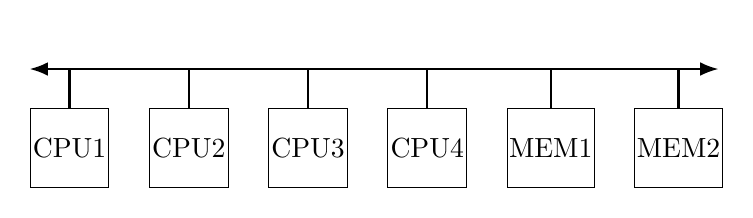
\begin{tikzpicture}
\matrix[
    matrix of nodes,
    nodes in empty cells,
    row 1/.style={nodes={minimum height=1cm,minimum width=1cm}},
    row 2/.style={nodes={draw,rectangle,minimum height=1cm,minimum width=1cm}},
    column sep=5mm,
] (net) {
      \& \& \& \& \&  \\
    CPU1 \& CPU2 \& CPU3 \& CPU4 \& MEM1 \& MEM2\\
};
\foreach \x in {1,2,3,4,5,6} {
    \draw[thick] (net-2-\x.north) -- (net-1-\x.center);
}
\draw[thick,Latex-Latex] (net-1-1.west) -- (net-1-6.east);
\end{tikzpicture}
\begin{itemize}
\item \myemph{tagged} messages --- everyone gets everything, filters
\item contention if multiple communicators
    \begin{itemize}
    \item some hardware enforces only one at a time
    \end{itemize}
\end{itemize}
\end{frame}

\begin{frame}{shared buses and scaling}
    \begin{itemize}
    \item shared buses perform poorly with ``too many'' CPUs
    \item so, there are other designs
        \vspace{.5cm}
    \item we'll gloss over these for now
    \end{itemize}
\end{frame}

\begin{frame}{shared buses and caches}
    \begin{itemize}
    \item remember caches?
    \item memory is \myemph{pretty slow}
    \item each CPU wants to keep local copies of memory
        \vspace{.5cm}
    \item what happens when multiple CPUs cache same memory?
    \end{itemize}
\end{frame}


\subsection{problem setup / snooping}
\input{../sync/cache-coherency-intro}

\section{aside: reordering}

\section{revisiting atomicity}
\subsection{processor reordering}
\begin{frame}[fragile,label=loadReorderSetup]{a simple race}
\begin{minipage}{0.45\textwidth}
\begin{lstlisting}[language=myasm,style=smaller]
thread_A:
    movl $1, x   /* x <- 1 */
    movl y, %eax /* return y */
    ret
\end{lstlisting}
\end{minipage}
\begin{minipage}{0.45\textwidth}
\begin{lstlisting}[language=myasm,style=smaller]
thread_B:
    movl $1, y   /* y <- 1 */
    movl x, %eax /* return x */
    ret
\end{lstlisting}
\end{minipage}
\\
\begin{lstlisting}[language=C++,style=smaller]
x = y = 0;
pthread_create(&A, NULL, thread_A, NULL);
pthread_create(&B, NULL, thread_B, NULL);
pthread_join(A, &A_result); pthread_join(B, &B_result);
printf("A:%d B:%d\n", (int) A_result, (int) B_result);
\end{lstlisting}
\begin{itemize}
\item<2-> if loads/stores atomic, then possible results:
    \begin{itemize}
    \item A:1 B:1 --- both moves into x and y, then both moves into eax execute
    \item A:0 B:1 --- thread A executes before thread B
    \item A:1 B:0 --- thread B executes before thread A
    \end{itemize}
\end{itemize}
\end{frame}

\begin{frame}[fragile,label=loadReorderExpResults]{a simple race: results}
\begin{minipage}{0.45\textwidth}
\begin{lstlisting}[language=myasm,style=smaller]
thread_A:
    movl $1, x   /* x <- 1 */
    movl y, %eax /* return y */
    ret
\end{lstlisting}
\end{minipage}
\begin{minipage}{0.45\textwidth}
\begin{lstlisting}[language=myasm,style=smaller]
thread_B:
    movl $1, y   /* y <- 1 */
    movl x, %eax /* return x */
    ret
\end{lstlisting}
\end{minipage}
\begin{lstlisting}[language=C++,style=smaller]
x = y = 0;
pthread_create(&A, NULL, thread_A, NULL);
pthread_create(&B, NULL, thread_B, NULL);
pthread_join(A, &A_result); pthread_join(B, &B_result);
printf("A:%d B:%d\n", (int) A_result, (int) B_result);
\end{lstlisting}
\vspace{-.5cm}
\begin{center}
\small my desktop, 100M trials: \\
\begin{tabular}{r|l|l}
frequency & result & ~ \\ \hline
$99\,823\,739$ & A:0 B:1 & (`A executes before B') \\
$171\,161$& A:1 B:0 & (`B executes before A') \\
$4\,706$ & A:1 B:1 & (`execute moves into x+y first') \\
\myemph<2>{$394$} & \myemph<2>{A:0 B:0} & \myemph<2>{???} \\
\end{tabular}
\end{center}
\end{frame}


\subsection{why reorder?}

\begin{frame}[fragile]{why reorder here?}
\begin{tikzpicture}
\node (thread A code) {
\begin{lstlisting}[language=myasm,style=smaller]
thread_A:
    movl $1, x   /* x <- 1 */
    movl y, %eax /* return y */
    ret
\end{lstlisting}
};
\node[anchor=north west] (thread B code) at ([xshift=.5cm]thread A code.north east) {
\begin{lstlisting}[language=myasm,style=smaller]
thread_B:
    movl $1, y   /* y <- 1 */
    movl x, %eax /* return x */
    ret
\end{lstlisting}
};
\end{tikzpicture}
\begin{itemize}
\item thread A: faster to load \texttt{y} right now!
\item \ldots rather than wait for write of \texttt{x} to finish
\end{itemize}
\end{frame}


\usetikzlibrary{calc}

\begin{frame}{why load/store reordering?}
\begin{itemize}
\item fast processor designs can execute instructions out of order
\item goal: do something instead of waiting for slow memory accesses, etc.
\item more on this later in the semester
\end{itemize}
\end{frame}



\subsection{compiler reordering}
\begin{frame}[fragile,label=compReorder]{compilers move loads/stores (1)}
\begin{lstlisting}[language=C++,style=small,
    moredelim={**[is][\btHL<2|handout:2>]{@2}{2@}},
    moredelim={**[is][\btHL<3|handout:3>]{@3}{3@}},
    moredelim={**[is][\btHL<4|handout:4>]{@4}{4@}},
    moredelim={**[is][\btHL<5|handout:5>]{@5}{5@}},
]
void Alice() {
    note_from_alice = 1;
    @2do {} while (note_from_bob);2@
    if (no_milk) {++milk;}
}
\end{lstlisting}
\hrule
\begin{lstlisting}[language=myasm,style=smaller,
    moredelim={**[is][\btHL<2|handout:2>]{@2}{2@}},
    moredelim={**[is][\btHL<3|handout:3>]{@3}{3@}},
    moredelim={**[is][\btHL<4|handout:4>]{@4}{4@}},
    moredelim={**[is][\btHL<5|handout:5>]{@5}{5@}},
]
Alice:
  movl $1, note_from_alice  // note_from_alice <- 1
  movl note_from_bob, %eax  // eax <- note_from_bob
.L2:
  @2testl %eax, %eax2@
  @2jne .L22@                   // while (eax == 0) repeat
  cmpl $0, no_milk          // if (no_milk != 0) ...
  ...
\end{lstlisting}
\end{frame}

\begin{frame}[fragile,label=compReorder2]{compilers move loads/stores too (2)}
\begin{lstlisting}[language=C++,style=smaller,
    moredelim={**[is][\btHL<2|handout:2>]{@2}{2@}},
    moredelim={**[is][\btHL<3|handout:3>]{@3}{3@}},
    moredelim={**[is][\btHL<4|handout:4>]{@4}{4@}},
    moredelim={**[is][\btHL<5|handout:5>]{@5}{5@}},
]
void Alice() {
    @3note_from_alice = 1;3@  // "Alice waiting" signal for Bob()
    do {} while (note_from_bob);
    if (no_milk) {++milk;}
    @2note_from_alice = 2;2@
}
\end{lstlisting}
\hrule
\begin{lstlisting}[language=myasm,style=smaller,
    moredelim={**[is][\btHL<2|handout:2>]{@2}{2@}},
    moredelim={**[is][\btHL<3|handout:3>]{@3}{3@}},
    moredelim={**[is][\btHL<4|handout:4>]{@4}{4@}},
    moredelim={**[is][\btHL<5|handout:5>]{@5}{5@}},
]
Alice:  
  // compiler optimization: don't set note_from_alice to 1,
  // (why? it will be set to 2 anyway)
  @3movl note_from_bob, %eax3@  // eax <- note_from_bob
.L2:
  testl %eax, %eax          
  jne .L2                   // while (eax == 0) repeat
  ...
  @2movl $2, note_from_alice2@  // note_from_alice <- 2
\end{lstlisting}
\end{frame}



\section{pthreads and load/store reordering}
\begin{frame}{pthreads and reordering}
    \begin{itemize}
    \item many pthreads functions \myemph{prevent reordering}
        \begin{itemize}
        \item everything before function call actually happens before 
        \end{itemize}
    \item includes \myemph{preventing some optimizations}
        \begin{itemize}
        \item e.g. keeping global variable in register for too long
        \end{itemize}
    \vspace{.5cm}
    \item pthread\_mutex\_lock/unlock, pthread\_create, pthread\_join, \ldots
        \begin{itemize}
        \item basically: if pthreads is waiting for/starting something, no weird ordering
        \end{itemize}
    \item implementation part 1: prevent compiler reordering
    \item implementation part 2: use special instructions
        \begin{itemize}
        \item example: x86 \texttt{mfence} instruction
        \end{itemize}
    \end{itemize}
\end{frame}




\begin{frame}{mfence}
    \begin{itemize}
        \item x86 instruction \texttt{mfence}
        \item make sure all loads/stores in progress finish
        \item \ldots and make sure no loads/stores were started early
            \vspace{.5cm}
        \item fairly expensive 
            \begin{itemize}
            \item Intel `Skylake': order 33 cycles + time waiting for pending stores/loads
            \end{itemize}
        \vspace{.5cm}
        \item<2-> aside: this instruction is did not exist in the original x86 \\
                so xv6 uses something older that's equivalent
    \end{itemize}
\end{frame}




\section{false sharing}
\begin{frame}{modifying cache blocks in parallel}
\begin{itemize}
\item cache coherency works on \myemph{cache blocks}
\item but typical memory access --- less than cache block
    \begin{itemize}
    \item e.g. one 4-byte array element in 64-byte cache block
    \end{itemize}
\vspace{.5cm}
\item what if two processors modify different parts same cache block?   
    \begin{itemize}
    \item 4-byte writes to 64-byte cache block
    \end{itemize}
\item cache coherency --- write instructions happen one at a time:
    \begin{itemize}
    \item processor `locks' 64-byte cache block, fetching latest version
    \item processor updates 4 bytes of 64-byte cache block
    \item later, processor might give up cache block
    \end{itemize}
\end{itemize}
\end{frame}

\begin{frame}[fragile,label=paralleModCode]{modifying things in parallel (code)}
\begin{lstlisting}[language=C++,style=smaller]
void *sum_up(void *raw_dest) {
    int *dest = (int *) raw_dest;
    for (int i = 0; i < 64 * 1024 * 1024; ++i) {
        *dest += data[i];
    }
}

__attribute__((aligned(4096))) 
int array[1024];  /* aligned = address is mult. of 4096 */

void sum_twice(int distance) {
    pthread_t threads[2];
    pthread_create(&threads[0], NULL, sum_up, &array[0]);
    pthread_create(&threads[1], NULL, sum_up, &array[distance]);
    pthread_join(threads[0], NULL);
    pthread_join(threads[1], NULL);
}
\end{lstlisting}
\end{frame}

\begin{frame}{performance v. array element gap}
(assuming \texttt{sum\_up} compiled to not omit memory accesses)
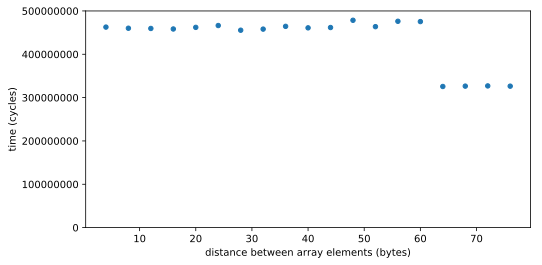
\includegraphics[width=\textwidth]{../sync/sum-up}
\end{frame}

\begin{frame}{false sharing}
\begin{itemize}
\item synchronizing to access two independent things
\vspace{.5cm}
\item two parts of same cache block
\item solution: separate them
\end{itemize}
\end{frame}


\subsection{exercise}
\begin{frame}[fragile,label=falseSharingEx1]{exercise (1)}
\begin{lstlisting}[
    language=C++,basicstyle=\tt\fontsize{9}{10}\selectfont,
    moredelim={**[is][\btHL<0|handout:0>]{@2}{2@}},
    moredelim={**[is][\btHL<0|handout:0>]{@3}{3@}},
    moredelim={**[is][\btHL<0|handout:0>]{@4}{4@}},
    escapeinside=QQ,
]
int @2values[1024]2@;
int @2results[2]2@;
void *sum_front(void *ignored_argument) {
    results[0] = 0;
    for (int i = @303@; i < @35123@; ++i)
        results[0] += values[i];
    return NULL;
}
void *sum_back(void *ignored_argument) {
    results[1] = 0;
    for (int i = @35123@; i < @310243@; ++i)
        results[1] += values[i];
    return NULL;
}
int sum_all() {
    pthread_t sum_front_thread, sum_back_thread;
    pthread_create(&sum_front_thread, NULL, sum_front, NULL);
    pthread_create(&sum_back_thread, NULL, sum_back, NULL);
    pthread_join(sum_front_thread, NULL);
    pthread_join(sum_back_thread, NULL);
    return @4results[0] + results[1]4@;
}
\end{lstlisting}
Where is false sharing likely to occur? How to fix?
\end{frame}

\begin{frame}[fragile,label=falseSharingEx2]{exercise (2)}
\begin{lstlisting}[
    language=C++,basicstyle=\tt\fontsize{9}{10}\selectfont,
    moredelim={**[is][\btHL<0|handout:0>]{@2}{2@}},
    moredelim={**[is][\btHL<0|handout:0>]{@3}{3@}},
    moredelim={**[is][\btHL<0|handout:0>]{@4}{4@}},
    escapeinside=QQ,
]
struct ThreadInfo { @2int *values;2@ int start; int end; int result };
void *sum_thread(void *argument) {
    ThreadInfo *@3my_info3@ = (ThreadInfo *) argument;Q\tikzmark{info}Q
    int sum = 0;
    for (int i = my_info->start; i < my_info->end; ++i) {
        my_info->result += my_info->values[i];
    }
    return NULL;

}
int sum_all(int *values) {
    ThreadInfo info[2]; pthread_t thread[2];
    for (int i = 0; i < 2; ++i) {
        @2info[i].values = values;2@ info[i].start = i*512; info[i].end = (i+1)*512;
        pthread_create(&threads[i], NULL, sum_thread, (void *) &info[i]);
    }
    for (int i = 0; i < 2; ++i)
        pthread_join(threads[i], NULL);
    return info[0].result + info[1].result;
}
\end{lstlisting}
Where is false sharing likely to occur?
\end{frame}

\section{recall: POSIX mutexes}

\begin{frame}[fragile,label=pthreadMutexBasic]{recall: pthread mutex}
\begin{lstlisting}[language=C++,style=small]
#include <pthread.h>

pthread_mutex_t some_lock;
pthread_mutex_init(&some_lock, NULL);
// or: pthread_mutex_t some_lock = PTHREAD_MUTEX_INITIALIZER;
...
pthread_mutex_lock(&some_lock);
...
pthread_mutex_unlock(&some_lock);
pthread_mutex_destroy(&some_lock);
\end{lstlisting}
\end{frame}



\subsection{pthread\_mutex: lock where you unlock}
\begin{frame}{POSIX mutex restrictions}
\begin{itemize}
\item pthread\_mutex rule: \myemph{unlock from same thread you lock in}
\vspace{.5cm}
\item implementation I gave before --- not a problem
\item \ldots but there other ways to implement mutexes
    \begin{itemize}
    \item e.g. might involve comparing with ``holding'' thread ID
    \end{itemize}
\end{itemize}
\end{frame}


\section{producer/consumer problem}
\usetikzlibrary{arrows.meta,shapes.multipart}

\begin{frame}{example: producer/consumer}
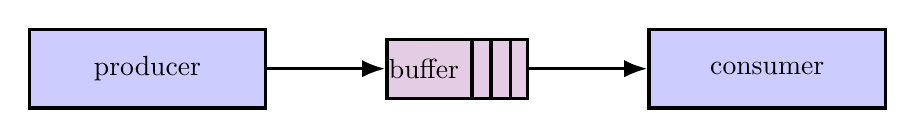
\begin{tikzpicture}
    \node[minimum width=3cm,minimum height=1cm,draw,very thick,fill=blue!20] (producer) {producer};
    \node[minimum height=0.75cm,draw,very thick,fill=violet!20,
          anchor=west,rectangle split,rectangle split horizontal,
          rectangle split parts=4] (buffer) at ([xshift=1.5cm]producer.east) {buffer
            \hspace{3cm}};
    \node[minimum width=3cm,minimum height=1cm,draw,very thick,fill=blue!20,
          anchor=west] (consumer) at ([xshift=1.5cm]buffer.east) {consumer};

    \begin{scope}[very thick,>=Latex]
        \draw[->] (producer)  -- (buffer);
        \draw[->] (buffer)  -- (consumer);
    \end{scope}
\end{tikzpicture}
    \begin{itemize}
        \item shared buffer (queue) of fixed size
            \begin{itemize}
            \item one or more producers inserts into queue
            \item one or more consumers removes from queue
            \end{itemize}
        \item<2-> producer(s) and consumer(s) don't work in lockstep
            \begin{itemize}
            \item (might need to wait for each other to catch up)
            \end{itemize}
        \item<3-> example: C compiler
            \begin{itemize}
            \item preprocessor $\rightarrow$ compiler $\rightarrow$ assembler $\rightarrow$ linker
            \end{itemize}
    \end{itemize}
\end{frame}



\section{monitors}

\subsection{introduction}
\usetikzlibrary{arrows.meta,calc,chains,fit,matrix}

\begin{frame}{monitors/condition variables}
\begin{itemize}
\item \myemph{locks} for mutual exclusion
\item \myemph{condition variables} for waiting for event
    \begin{itemize}
    \item operations: wait (for event); signal/broadcast (that event happened)
    \end{itemize}
\item related data structures
\vspace{.5cm}
\item \myemph{monitor} = lock + 0 or more condition variables + shared data
    \begin{itemize}
    \item Java: every object is a monitor (has instance variables, built-in lock, cond. var)
    \item pthreads: build your own: provides you locks + condition variables
    \end{itemize}
\end{itemize}
\end{frame}

\begin{frame}[fragile,label=monitorIdea]{monitor idea}
\begin{tikzpicture}
\tikzset{
    hilite red on/.style={alt=<#1>{fill=red!10}},
    hilite blue on/.style={alt=<#1>{fill=blue!10}},
    >=Latex,
    queue node/.style={draw,thick,minimum width=.6cm,minimum height=.6cm},
    queue connect/.style={draw,->,ultra thick},
}
\matrix[
    tight matrix,
    nodes={draw,thick,text width=4cm,font=\small},
    label={[font=\small]north:a monitor},
    ] (monitor) {
    |[hilite red on={2-}]| lock \\
    shared data \\
    |[hilite blue on={4-}]| condvar 1 \\
    |[hilite blue on={4-}]| condvar 2 \\
    \ldots \\
    |[minimum height=0.2mm]| {} \\
    operation1(\ldots)\\
    operation2(\ldots) \\
};
\begin{visibleenv}<2-3|handout:2>
    \node[draw=red,ultra thick,inner sep=0mm,fit=(monitor-2-1) (monitor-5-1)] {};
\end{visibleenv}
\begin{visibleenv}<2|handout:0>
    \node[red,anchor=north west,align=left] at (monitor-1-1.north east) {
            lock must be acquired \\
            before accessing \\
            any part of monitor's stuff
    };
\end{visibleenv}
\begin{visibleenv}<3->
    \begin{scope}[
        start chain=going right,
        every join/.style={queue connect},
        every node/.style={queue node,on chain,join,fill=red!10},
    ]
    \node[anchor=west] (lock queue 1) at ([xshift=1cm]monitor-1-1.east) {};
    \node (lock queue 2) {};
    \node (lock queue 3) {};
    \end{scope}
    \draw[->,dashed,ultra thick] (monitor-1-1) -- (lock queue 1);
\end{visibleenv}
\begin{visibleenv}<3->
    \node[anchor=west,align=left,text=red!20!black] at ([xshift=0cm]lock queue 3.east) {
        threads waiting for lock
    };
\end{visibleenv}
\begin{visibleenv}<4->
    \begin{scope}[
        start chain=going right,
        every join/.style={queue connect},
        every node/.style={queue node,on chain,join,fill=blue!10},
    ]
    \node[anchor=west] (condvar 1 queue 1) at ([xshift=1cm,yshift=-1cm]monitor-3-1.east) {};
    \node (condvar 1 queue 2) {};
    \node (condvar 1 queue 3) {};
    \end{scope}
    \draw[->,dashed,ultra thick] (monitor-3-1.east) -- (condvar 1 queue 1);

    \begin{scope}[
        start chain=going right,
        every join/.style={queue connect},
        every node/.style={queue node,on chain,join,fill=blue!10},
    ]
    \node[anchor=west] (condvar 2 queue 1) at ([xshift=1cm,yshift=-1.5cm]monitor-4-1.east) {};
    \node (condvar 2 queue 2) {};
    \node (condvar 2 queue 3) {};
    \end{scope}
    \draw[->,dashed,ultra thick] (monitor-4-1.east) -- (condvar 2 queue 1);
    \node[anchor=west,align=left,text=blue!20!black] at ($(condvar 2 queue 3.north east)!0.5!(condvar 1 queue 3.south east)$) {
        threads waiting for \\
        condition to be true \\ 
        about shared data
    };
\end{visibleenv}
\end{tikzpicture}
\end{frame}

\begin{frame}[fragile,label=condVarOps]{condvar operations}
\begin{tikzpicture}
\tikzset{
    hilite red on/.style={alt=<#1>{fill=red!10}},
    hilite blue on/.style={alt=<#1>{fill=blue!10}},
    >=Latex,
    queue node/.style={draw,thick,minimum width=.6cm,minimum height=.6cm},
    queue connect/.style={draw,->,ultra thick},
}
\matrix[
    tight matrix,
    nodes={draw,thick,text width=4cm,font=\small},
    label={[font=\small]north:a monitor},
    ] (monitor) {
    |[hilite red on={1-}]| lock \\
    shared data \\
    |[hilite blue on={1-}]| condvar 1 \\
    |[hilite blue on={1-}]| condvar 2 \\
    \ldots \\
    |[minimum height=0.2mm]| {} \\
    operation1(\ldots)\\
    operation2(\ldots) \\
};
    %\node[draw=red,ultra thick,inner sep=0mm,fit=(monitor-2-1) (monitor-5-1)] {};
    \begin{scope}[
        start chain=going right,
        %every join/.style={queue connect},
        every node/.style={queue node,on chain,fill=red!10},
    ]
    \node[anchor=west,alt=<3>{opacity=0.2}] (lock queue 1) at ([xshift=1cm]monitor-1-1.east) {};
    \node (lock queue 2) {};
    \node (lock queue 3) {};
    \end{scope}
    \draw[queue connect,alt=<3>{opacity=0.2}] (lock queue 1) --(lock queue 2);
    \draw[queue connect] (lock queue 2) --(lock queue 3);
    \draw[->,dashed,ultra thick,alt=<3>{opacity=0}] (monitor-1-1) -- (lock queue 1);
    \begin{visibleenv}<3>
        \draw[->,dashed,ultra thick,red,out=-15,in=-155] (monitor-1-1.east) to (lock queue 2);
    \end{visibleenv}
    \node[anchor=west,align=left,text=red!20!black] at ([xshift=0cm]lock queue 3.east) {
        threads waiting for lock
    };
    \begin{scope}[
        start chain=going right,
        every join/.style={queue connect,alt={<4,5>{opacity=0.2}}},
        every node/.style={queue node,on chain,join,fill=blue!10,alt=<4>{draw=red,dashed,thick}},
    ]
    \node[anchor=west] (condvar 1 queue 1) at ([xshift=1cm,yshift=-1cm]monitor-3-1.east) {};
    \node[alt=<5>{draw=red,dashed,thick}] (condvar 1 queue 2) {};
    \node (condvar 1 queue 3) {};
    \end{scope}
    \draw[->,dashed,ultra thick,alt=<4>{opacity=0.2}] (monitor-3-1.east) -- (condvar 1 queue 1);
    \begin{visibleenv}<5>
        \draw[->,dashed,ultra thick,red,in=-155,out=-20] (condvar 1 queue 1) to (condvar 1 queue 3);
    \end{visibleenv}

    \begin{scope}[
        start chain=going right,
        every join/.style={queue connect},
        every node/.style={queue node,on chain,join,fill=blue!10},
    ]
    \node[anchor=west] (condvar 2 queue 1) at ([xshift=1cm,yshift=-1.5cm]monitor-4-1.east) {};
    \node (condvar 2 queue 2) {};
    \node (condvar 2 queue 3) {};
    \end{scope}
    \draw[->,dashed,ultra thick] (monitor-4-1.east) -- (condvar 2 queue 1);
    \node[anchor=west,align=left,text=blue!20!black] at ($(condvar 2 queue 3.north east)!0.5!(condvar 1 queue 3.south east)$) {
        threads waiting for \\
        condition to be true \\ 
        about shared data
    };
    \node[anchor=south west,align=left] (oplist)  at ([yshift=.5cm,xshift=-3.5cm]monitor.north east) {
        \textcolor{blue!80!black}{condvar} operations: \\
        \myemph<2-3>{\textbf<2>{Wait(cv, lock)}} --- \myemph<3>{unlock} lock, \myemph<2>{add current thread} to cv queue \\
        \ldots and \myemph<3>{reacquire} lock before returning \\
        \myemph<4>{\textbf<4>{Broadcast(cv)}} --- remove all from condvar queue \\
        \myemph<5>{\textbf<5>{Signal(cv)}} --- remove one from condvar queue \\
    };
    \tikzset{
        queue change/.style={dashed,ultra thick,red},
    }
    \begin{visibleenv}<3>
        \draw[->,queue change,in=180,out=90] (lock queue 1.north) to ++(1cm,1cm)
            node[right,red,font=\small] {unlock lock --- allow thread from queue to go};
    \end{visibleenv}
    \begin{visibleenv}<2>
        \draw[->,queue change,in=180,out=90] (condvar 1 queue 3.north) to ++(1cm,1cm) node[right,queue node,draw=red,
            label={[font=\small]east:calling thread starts waiting}] {};
    \end{visibleenv}
    \begin{visibleenv}<3>
        \draw[->,black!50,in=180,out=90] (condvar 1 queue 3.north) to ++(1cm,1cm) node[right,queue node,draw=red,
            ] {};
    \end{visibleenv}
    \begin{visibleenv}<4>
        \coordinate (unqueue dest) at (lock queue 3.south);
        \draw[<-,queue change,in=-90,out=90] (condvar 1 queue 1.north) to (unqueue dest);
        \draw[<-,queue change,in=90,out=90] (condvar 1 queue 2.north) to (condvar 1 queue 1.north);
        \draw[<-,queue change,in=90,out=90] (condvar 1 queue 3.north) to (condvar 1 queue 2.north);
        \node[anchor=north west,text=red,font=\small,align=left] at (unqueue dest) {
            all threads removed from cv queue \\
            to start waiting for lock
        };
    \end{visibleenv}
    \begin{visibleenv}<5>
        \coordinate (unqueue dest) at (lock queue 3.south);
        \draw[<-,queue change,in=-90,out=90] (condvar 1 queue 2.north) to (unqueue dest);
        \node[anchor=north west,text=red,font=\small,align=left] at (unqueue dest) {
            any one thread removed from cv queue \\
            to start waiting for lock
        };
    \end{visibleenv}
\end{tikzpicture}
\end{frame}
  % FIXME: incomplete

\subsection{example: WaitForFinished}
\begin{frame}[fragile,label=finishedExample]{pthread cv usage}
\begin{lstlisting}[
    language=C++,style=size105,
    morekeywords={pthread_mutex_t,pthread_cond_t},
    moredelim={**[is][\btHL<2|handout:2>]{@2}{2@}}, 
    moredelim={**[is][\btHL<3|handout:3>]{@3}{3@}}, 
    moredelim={**[is][\btHL<4|handout:4>]{@4}{4@}}, 
    moredelim={**[is][\btHL<5|handout:5>]{@5}{5@}}, 
    escapeinside=QQ,
]
// MISSING: init calls, etc.
pthread_mutex_t lock;
bool finished;   // data, only accessed with after acquiring lock
pthread_cond_t finished_cv;  // to wait for 'finished' to be true

void WaitForFinished() {
  @2pthread_mutex_lock(&lock);2@Q\tikzmark{lock for wait}Q
  @3while (!finished) {3@Q\tikzmark{finished loop}Q
    @4pthread_cond_wait(&finished_cv, &lock);4@Q\tikzmark{wait}Q
  }
  pthread_mutex_unlock(&lock);
}

void Finish() {
  @2pthread_mutex_lock(&lock);2@Q\tikzmark{lock for finish}Q
  finished = true;
  @5pthread_cond_broadcast(&finished_cv);5@Q\tikzmark{broadcast}Q
  pthread_mutex_unlock(&lock);
}
\end{lstlisting}
\begin{tikzpicture}[overlay,remember picture]
\tikzset{
    >=Latex,
    explain box/.style={draw=red,text=black,very thick,align=left},
    point line/.style={very thick,red},
}

\begin{visibleenv}<2>
    \node[explain box,anchor=east,fill=white] (acquire text) at ([yshift=-1cm,xshift=-.5cm]current page.east) {
        acquire lock before \\ reading or writing \texttt{finished}
    };
    \draw[point line,<-] ([yshift=1.5mm]pic cs:lock for wait) -- (acquire text);
    \draw[point line,<-] ([yshift=1.5mm]pic cs:lock for finish) -- (acquire text);
\end{visibleenv}
\begin{visibleenv}<3>
    \node[explain box,anchor=east,fill=white,fill opacity=0.9] (loop text) at ([xshift=-.5cm]current page.east |- {pic cs:finished loop}) {
        check whether we need to wait at all \\
        {\small (why a loop? we'll explain later)}
    };
    \draw[point line,<-] ([yshift=1.5mm]pic cs:finished loop) -- (loop text);
\end{visibleenv}
\begin{visibleenv}<4>
    \node[explain box,anchor=east,fill=white,fill opacity=0.9] (wait text) at ([xshift=-.5cm,yshift=-2cm]current page.east) {
        know we need to wait  \\
        (finished can't change while we have lock) \\
        so wait, releasing lock\ldots
    };
    \draw[point line,<-] ([yshift=1.5mm]pic cs:wait) -- (wait text);
\end{visibleenv}
\begin{visibleenv}<5>
    \node[explain box,anchor=east,fill=white,fill opacity=0.9] (broadcast text) at ([yshift=2cm,xshift=-.5cm]current page.east |- {pic cs:broadcast}) {
        allow all waiters to proceed \\
        (once we unlock the lock)
    };
    \draw[point line,<-] ([yshift=1.5mm]pic cs:broadcast) -- (broadcast text);
\end{visibleenv}
\end{tikzpicture}
\end{frame}

\begin{frame}[fragile,label=waitForFinishTimeline1]{WaitForFinish timeline 1}
\lstset{language=C++,style=smaller}
\small
  \vspace{-.25cm}
\begin{tabular}{l|l}
  \textbf{WaitForFinish thread} & \textbf{Finish thread} \\ \hline\hline
\lstinline|mutex_lock(&lock)| & \\
(thread has lock)             & \\ \hline
~                             & \lstinline|mutex_lock(&lock)|  \\
~                             & (start waiting for lock)\\ \hline
\lstinline|while (!finished) ...| & \\
\lstinline|cond_wait(&finished_cv, &lock);| & \\
(start waiting for cv) & (done waiting for lock) \\ \hline
~ & \lstinline|finished = true| \\
~ & \lstinline|cond_broadcast(&finished_cv)| \\ \hline
(done waiting for cv) & ~ \\
(start waiting for lock) & ~ \\ \hline
~ & \lstinline|mutex_unlock(&lock)| \\ \hline
(done waiting for lock) \\
\lstinline|while (!finished) ...| & \\
(finished now true, so return) \\
\lstinline|mutex_unlock(&lock)| \\
\end{tabular}
\end{frame}

\begin{frame}[fragile,label=waitForFinishTimeline2]{WaitForFinish timeline 2}
\lstset{language=C++,style=smaller}
\small
  \vspace{-.25cm}
\begin{tabular}{l|l}
  \textbf{WaitForFinish thread} & \textbf{Finish thread} \\ \hline\hline
~                             & \lstinline|mutex_lock(&lock)|  \\
~                             & \lstinline|finished = true| \\ 
~                             & \lstinline|cond_broadcast(&finished_cv)| \\ 
~                             & \lstinline|mutex_unlock(&lock)| \\ \hline
\lstinline|mutex_lock(&lock)| & \\
\lstinline|while (!finished) ...| & \\
(finished now true, so return) \\
\lstinline|mutex_unlock(&lock)| \\
\end{tabular}
\end{frame}

\begin{frame}[fragile,label=whyLoop]{why the loop}
\begin{lstlisting}[language=C++,style=small]
while (!finished) {
  pthread_cond_wait(&finished_cv, &lock);
}
\end{lstlisting}
\begin{itemize}
  \item we only \texttt{broadcast} if \texttt{finished} is true
  \item so why check \texttt{finished} afterwards?
    \vspace{.5cm}

  \item<2-> pthread\_cond\_wait manual page: 
        \begin{itemize}
          \item ``\myemph{Spurious wakeups} ... may occur.''
            \end{itemize}
  \item<2-> spurious wakeup = \texttt{wait} returns even though nothing happened
\end{itemize}
\end{frame}



\subsection{unbounded queue with monitors}
\usetikzlibrary{arrows.meta,fit,matrix}

\begin{frame}[fragile,label=unboundedPC]{unbounded buffer producer/consumer}
\begin{lstlisting}[
    language=C++,
    basicstyle=\tt\fontsize{10}{11}\selectfont,
    morekeywords=pthread_mutex_t,
    morekeywords=pthread_cond_t,
    morekeywords=UnboundedQueue,
    moredelim={**[is][\btHL<2|handout:2>]{@2}{2@}},
    moredelim={**[is][\btHL<3|handout:3>]{@3}{3@}},
    moredelim={**[is][\btHL<4|handout:4>]{@4}{4@}},
    moredelim={**[is][\btHL<5-,3|handout:5-,3>]{@5}{5@}},
    escapeinside=XX,
]
pthread_mutex_t lock;
pthread_cond_t data_ready;
UnboundedQueue buffer;

Produce(item) {
    @2pthread_mutex_lock(&lock);2@
    buffer.enqueue(item);
    @4pthread_cond_signal(&data_ready);4@X\tikzmark{signal}X
    @2pthread_mutex_unlock(&lock);2@
}
Consume() {
    @2pthread_mutex_lock(&lock);2@
    while (@5buffer.empty()5@) {X\tikzmark{empty}X
        pthread_cond_wait(&data_ready, &lock);
    }X\tikzmark{after loop}X
    item = @3buffer.dequeue()3@;
    @2pthread_mutex_unlock(&lock);2@
    return item;
}
\end{lstlisting}
\begin{tikzpicture}[overlay,remember picture]
    \coordinate (place) at ([xshift=-.5cm,yshift=-1.5cm]current page.north east);
    \coordinate (place lower) at ([xshift=-.5cm,yshift=-4.25cm]current page.north east);
    \tikzset{
        box base/.style={draw=red,ultra thick,align=left,anchor=north east,fill=white},
        box/.style={box base,at={(place)}},
        box lower/.style={box base,at={(place lower)}},
        >=Latex,
    }
    \begin{visibleenv}<2>
        \node [box] {
            rule: never touch \texttt{buffer} \\
            without acquiring lock \\
            ~ \\
            otherwise: what if two threads \\ simultaneously en/dequeue?  \\
            {\small (both use same array/linked list entry?)} \\
            {\small (both reallocate array?)}
        };
    \end{visibleenv}
    \begin{visibleenv}<3>
        \node [box lower] {
            check if not empty \\
            if so, dequeue \\
            ~ \\
            okay because have lock
        };
        \draw[<-,very thick,draw=red] (pic cs:after loop) -- ++(6cm,0cm) node[right,align=left] {
            other threads can\textbf{not} dequeue here
        };
    \end{visibleenv}
    \begin{visibleenv}<4>
        \draw[<-,very thick,draw=red] ([yshift=1.5mm]pic cs:signal) -- ++(2cm,0cm) node[right,align=left] {
            wake one Consume thread \\ \textit{if any are waiting} \\
        };
    \end{visibleenv}
    \begin{visibleenv}<5->
        \draw[<-,very thick,draw=red] ([yshift=1.5mm]pic cs:empty) -- ++(1cm,-2cm)
        node[fill=white,draw=red,right,align=left,font=\fontsize{10.5}{10}\selectfont,inner sep=0.1mm] {
            \myemph<5>{0 iterations}: Produce() called before Consume() \\
            \myemph<6>{1 iteration}: Produce() signalled, probably \\
            \myemph<7-8>{2+ iterations}: spurious wakeup or \ldots?
        };
        \tikzset{
            timeline/.style={
                tight matrix,fill=white,
                nodes={text width=3.5cm,font=\fontsize{10.5}{11}\selectfont,fill=white,text depth=0.075cm,text height=0.25cm},
                at={([xshift=-0.75cm,yshift=-1.15cm]current page.north east)},
                anchor=north east,
                row 1/.style={nodes={font=\bfseries\small,draw=none,align=center}},
            },
            wait for lock/.style={
                draw,inner sep=0mm,
                text=black!70,
                align=center,
                fill=white,
                font=\fontsize{11}{12}\selectfont,
            }
        }
        \begin{visibleenv}<5>
            \matrix[timeline] {
                Thread 1 \& Thread 2 \\
                Produce() \\
                \ldots lock \\
                \ldots enqueue \\
                \ldots signal \\
                \ldots unlock \\
                \& Consume() \\
                \& \ldots lock \\
                \& |[fill=green!20]| \ldots empty? no \\
                \& \ldots dequeue \\
                \& \ldots unlock \\
                \& return \\
            };
        \end{visibleenv}
        \begin{visibleenv}<6>
            \matrix[timeline,column 1/.style={nodes={text width=2cm}}] (one wait timeline) {
                Thread 1 \& Thread 2 \\
                \& Consume() \\
                \& \ldots lock \\
                \& |[fill=red!20]| \ldots empty? yes \\
                 \& \ldots unlock/start wait \\
                Produce() \& ~\\
                \ldots lock \\
                \ldots enqueue \& ~\\
                \ldots signal \& stop wait \\
                \ldots unlock \& lock \\
                \& |[fill=green!20]| \ldots empty? no \\
                \& \ldots dequeue \\
                \& \ldots unlock \\
                \& return \\
            };
            \node[wait for lock,fit=(one wait timeline-6-2) (one wait timeline-8-2)] {
                waiting for \\
                data\_ready
            };
        \end{visibleenv}
        \begin{visibleenv}<7-8>
            \matrix[timeline,
                    column 1/.style={nodes={text width=2cm}},
                    column 3/.style={nodes={text width=2cm}},
                    ] (two wait timeline) {
                Thread 1 \& Thread 2 \& Thread 3\\
                \& Consume() \\
                \& \ldots lock \\
                \& |[fill=red!20]| \ldots empty? yes \\
                 \& \ldots unlock/start wait \\
                Produce() \& ~ \\
                \ldots lock \& \& Consume() \\
                \ldots enqueue \& ~ \& ~ \\
                |[alias=two signal]| \ldots signal \& |[alias=two stop wait]| stop wait \& ~ \\
                \ldots unlock \& ~ \& |[alt=<8>{draw=red}]| lock \\
                \& \& \ldots empty? no \\
                \& \& \ldots dequeue \\
                \& ~ \& \ldots unlock \\
                \& \ldots lock \& return  \\
                \& |[fill=red!20]| \ldots empty? yes \\
                \& \ldots unlock/start wait \\
            };
            \node[wait for lock,fit=(two wait timeline-6-2) (two wait timeline-8-2)] {
                waiting for \\
                data\_ready
            };
            \node[wait for lock,fit=(two wait timeline-10-2) (two wait timeline-13-2)] {
                waiting for \\
                lock
            };
            \node[wait for lock,fit=(two wait timeline-8-3) (two wait timeline-9-3),
                  label={[font=\fontsize{11}{12}\selectfont,black!70,align=center]center:waiting for\\lock}] {};
            \begin{visibleenv}<8>
                \node[draw=red,thick,inner sep=0mm,fit=(two signal) (two stop wait)] (mark stop wait) {};
                \draw[thick,red,<-] (mark stop wait.west) -- ++(-1cm,0cm) node[draw=red,text=black,font=\small,left,fill=white,align=right] {
                    in pthreads: signaled thread not \\
                    guaranteed to hold lock next \\
                    ~ \\
                    alternate design: \\
                    signaled thread gets lock next \\
                    called ``Hoare scheduling'' \\
                    not done by pthreads, Java, \ldots
                };
            \end{visibleenv}
        \end{visibleenv}
    \end{visibleenv}
\end{tikzpicture}
\end{frame}


\subsection{Hoare scheduling note}
\begin{frame}{Hoare versus Mesa monitors}
\begin{itemize}
\item Hoare-style monitors
    \begin{itemize}
    \item signal `hands off' lock to awoken thread
    \end{itemize}
\item Mesa-style monitors
    \begin{itemize}
    \item any eligible thread gets lock next
    \item (maybe some other idea of priority?)
    \end{itemize}
\vspace{.5cm}
\item every current threading library I know of does Mesa-style
\end{itemize}
\end{frame}


\subsection{bounded producer/consumer with monitors}
\usetikzlibrary{arrows.meta,fit,matrix}

\begin{frame}[fragile,label=boundedPC]{bounded buffer producer/consumer}
\begin{lstlisting}[
    language=C++,
    basicstyle=\tt\fontsize{9.5}{10.5}\selectfont,
    morekeywords=pthread_mutex_t,
    morekeywords=pthread_cond_t,
    morekeywords=BoundedQueue,
    moredelim={**[is][\btHL<2|handout:2>]{@2}{2@}}, 
    moredelim={**[is][\btHL<2-3|handout:2-3>]{@3}{3@}}, 
    moredelim={**[is][\btHL<4|handout:4>]{@4}{4@}}, 
    escapeinside=XX,
]
pthread_mutex_t lock;
pthread_cond_t @4data_ready4@; @2pthread_cond_t @4space_ready4@;2@
BoundedQueue buffer;
Produce(item) {
    pthread_mutex_lock(&lock);
    @2while (buffer.full()) { pthread_cond_wait(@4&space_ready4@, &lock); }2@
    buffer.enqueue(item);
    pthread_cond_signal(@4&data_ready4@);
    pthread_mutex_unlock(&lock);
}
Consume() {
    pthread_mutex_lock(&lock);
    while (buffer.empty()) {
        pthread_cond_wait(@4&data_ready4@, &lock);
    }
    item = buffer.dequeue();
    @3pthread_cond_signal(@4&space_ready4@);3@X\tikzmark{signal}X
    pthread_mutex_unlock(&lock);
    return item;
}
\end{lstlisting}
\begin{tikzpicture}[overlay,remember picture]
\tikzset{
    >=Latex
}
\begin{visibleenv}<3>
\draw[draw=red,thick,<-] ([xshift=-2cm,yshift=3mm]pic cs:signal) -- ++(0cm,1cm) node[anchor=south,draw=red,text=black,fill=white,align=left] {
    correct (but slow?) to replace with: \\
\texttt{pthread\_cond\_broadcast(\&space\_ready);} \\
(just more ``spurious wakeups'')
};
\end{visibleenv}
\begin{visibleenv}<4>
\node[anchor=east,draw=red,thick,fill=white,font=\small,align=left] at ([yshift=-.5cm]current page.east) {
correct but slow to replace \\
\texttt{data\_ready} and \texttt{space\_ready} \\
with `combined' condvar \texttt{ready} \\
and use broadcast \\
(just more ``spurious wakeups'')
};
\end{visibleenv}
\end{tikzpicture}
\end{frame}
 

\subsection{general monitor pattern}
\begin{frame}[fragile,label=monitorPattern]{monitor pattern}
\begin{lstlisting}[language=C++,style=small]
pthread_mutex_lock(&lock);
while (!condition A) {
    pthread_cond_wait(&condvar_for_A, &lock);
}
... /* manipulate shared data, changing other conditions */
if (set condition A) {
    pthread_cond_broadcast(&condvar_for_A);
    /* or signal, if only one thread cares */
}
if (set condition B) {
    pthread_cond_broadcast(&condvar_for_B);
    /* or signal, if only one thread cares */
}
...
pthread_mutex_unlock(&lock)
\end{lstlisting}
\end{frame}

\begin{frame}[fragile,label=monitorRulesOfThumb]{monitors rules of thumb}
\begin{itemize}
\item never touch shared data without holding the lock
\item keep lock held for \myemph{entire operation}:
    \begin{itemize}
    \item verifying condition (e.g. buffer not full) \textit{up to and including}
    \item manipulating data (e.g. adding to buffer)
    \end{itemize}
\item create condvar for every kind of scenario waited for
\item always write \myemph{loop} calling cond\_wait to wait for condition X
\item broadcast/signal condition variable \myemph{every time you change X}
\item<2-> correct but slow to\ldots
    \begin{itemize}
    \item broadcast when just signal would work
    \item broadcast or signal when nothing changed
    \item use one condvar for multiple conditions
    \end{itemize}
\end{itemize}
\end{frame}


\subsection{monitor POSIX API details}
\begin{frame}[fragile,label=createMonitors]{mutex/cond var init/destroy}
\begin{lstlisting}[style=smaller]
pthread_mutex_t mutex;
pthread_cond_t cv;
pthread_mutex_init(&mutex, NULL);
pthread_cond_init(&cv, NULL);
// --OR--
pthread_mutex_t mutex = PTHREAD_MUTEX_INITIALIZER;
pthread_cond_t cv = PTHREAD_COND_INITIALIZER;

// and when done:
...
pthread_cond_destroy(&cv);
pthread_mutex_destroy(&mutex);
\end{lstlisting}
\end{frame}



\subsection{exercise: wait for both finished}
\usetikzlibrary{arrows.meta}
\begin{frame}[fragile,label=bothFinishedEx]{wait for both finished}
\begin{lstlisting}[
    language=C++,style=size105,
    morekeywords={pthread_mutex_t,pthread_cond_t},
    moredelim={**[is][\btHL<2|handout:2>]{@2}{2@}}, 
    moredelim={**[is][\btHL<3|handout:3>]{@3}{3@}}, 
    moredelim={**[is][\btHL<4|handout:4>]{@4}{4@}}, 
    moredelim={**[is][\btHL<5|handout:5>]{@5}{5@}}, 
    escapeinside=QQ,
]
// MISSING: init calls, etc.
pthread_mutex_t lock;
bool finished[2];
pthread_cond_t both_finished_cv;

void WaitForBothFinished() {
  pthread_mutex_lock(&lock);Q\tikzmark{lock for wait}Q
  while (@2_____________________________2@) {Q\tikzmark{finished loop}Q
    pthread_cond_wait(&both_finished_cv, &lock);Q\tikzmark{wait}Q
  }
  pthread_mutex_unlock(&lock);
}

void Finish(int index) {
  pthread_mutex_lock(&lock);Q\tikzmark{lock for finish}Q
  finished[index] = true;
  @3_____________________________________3@
  pthread_mutex_unlock(&lock);
}
\end{lstlisting}
\begin{tikzpicture}[overlay,remember picture]
\tikzset{
    >=Latex,
    explain box/.style={draw=red,text=black,very thick,align=left,font=\small},
    point line/.style={very thick,red},
}
\begin{visibleenv}<2>
    \node[explain box,anchor=north east] (acquire text) at ([yshift=-1cm,xshift=-.25cm]current page.north east) {
        A. \lstinline*finished[0] && finished[1]* \\
        B. \lstinline*finished[0] || finished[1]* \\
        C. \lstinline*!finished[0] || !finished[1]* \\
        D. \lstinline*finished[0] != finished[1]* \\
        E. something else
    };
\end{visibleenv}
\begin{visibleenv}<3>
    \node[explain box,anchor=north east,font=\fontsize{9}{10}\selectfont,fill=white] (acquire text) at ([yshift=-2cm,xshift=-.25cm]current page.north east) {
        A. \lstinline*pthread_cond_signal(&both_finished_cv)* \\
        B. \lstinline*pthread_cond_broadcast(&both_finished_cv)* \\
        C. \lstinline*if (finished[1-index])* \\
        \hspace{1.5cm} \lstinline*pthread_cond_signal(&both_finished_cv);* \\
        D. \lstinline*if (finished[1-index])* \\
        \hspace{1.5cm} \lstinline*pthread_cond_broadcast(&both_finished_cv);* \\
        E. something else
    };
\end{visibleenv}
\end{tikzpicture}
\end{frame}


\subsection{exercise: barrier}
\begin{frame}[fragile,label=monitorExercise2]{monitor exercise: barrier}
\begin{itemize}
\item suppose we want to implement a one-use barrier; fill in blanks:
\end{itemize}
\begin{lstlisting}[style=smaller]
struct BarrierInfo {
    pthread_mutex_t lock;
    int total_threads;  // initially total # of threads
    int number_reached; // initially 0
    ___________________
};

void BarrierWait(BarrierInfo *b) {
    pthread_mutex_lock(&b->lock);
    ++b->number_reached;
    if (b->number_reached == b->total_threads) {
        _____________________
    } else {
        _____________________
    }
    pthread_mutex_unlock(&b->lock);
}
\end{lstlisting}
\end{frame}


\subsection{exercise: ConsumeTwo}
\begin{frame}[fragile,label=monitorExercise]{monitor exercise: ConsumeTwo}
\begin{itemize}
\item suppose we want producer/consumer, but\ldots
\item but change Consume() to ConsumeTwo() which returns a \myemph{pair of values}
    \begin{itemize}
    \item and don't want two calls to ConsumeTwo() to wait\ldots
    \item with each getting one item
    \end{itemize}
\item what should we change below?
\end{itemize}
\begin{minipage}{0.45\textwidth}
\begin{lstlisting}[
    language=C++,
    basicstyle=\tt\fontsize{9.5}{10.5}\selectfont,
    morekeywords=pthread_mutex_t,
    morekeywords=pthread_cond_t,
    morekeywords=UnboundedQueue,
    moredelim={**[is][\btHL<2|handout:2>]{@2}{2@}}, 
    moredelim={**[is][\btHL<3|handout:3>]{@3}{3@}}, 
    moredelim={**[is][\btHL<4|handout:4>]{@4}{4@}}, 
    moredelim={**[is][\btHL<5-,3|handout:5-,3>]{@5}{5@}}, 
    escapeinside=XX,
]
pthread_mutex_t lock;
pthread_cond_t data_ready;
UnboundedQueue buffer;

Produce(item) {
  pthread_mutex_lock(&lock);
  buffer.enqueue(item);
  pthread_cond_signal(&data_ready);
  pthread_mutex_unlock(&lock);
}
\end{lstlisting}
\end{minipage}
\begin{minipage}{0.45\textwidth}
\begin{lstlisting}[
    language=C++,
    basicstyle=\tt\fontsize{9.5}{10.5}\selectfont,
    morekeywords=pthread_mutex_t,
    morekeywords=pthread_cond_t,
    morekeywords=UnboundedQueue,
    moredelim={**[is][\btHL<2|handout:2>]{@2}{2@}}, 
    moredelim={**[is][\btHL<3|handout:3>]{@3}{3@}}, 
    moredelim={**[is][\btHL<4|handout:4>]{@4}{4@}}, 
    moredelim={**[is][\btHL<5-,3|handout:5-,3>]{@5}{5@}}, 
    escapeinside=XX,
]
Consume() {
  pthread_mutex_lock(&lock);
  while (buffer.empty()) {
    pthread_cond_wait(&data_ready, &lock);
  }
  item = buffer.dequeue();
  pthread_mutex_unlock(&lock);
  return item;
}
\end{lstlisting}
\end{minipage}
\end{frame}

\iftoggle{heldback}{\excludecomment{isheldback}}{\includecomment{isheldback}}
\begin{isheldback}
\begin{frame}[fragile,label=monitorExerciseSln]{monitor exercise: solution (1)}
\small (one of many possible solutions) \\
Assuming ConsumeTwo \textbf{replaces} Consume:
\begin{lstlisting}[basicstyle=\tt\fontsize{9.5}{10.5}\selectfont]
Produce() {
  pthread_mutex_lock(&lock);
  buffer.enqueue(item);
  if (buffer.size() > 1) { pthread_cond_signal(&data_ready); }
  pthread_mutex_unlock(&lock);
}
ConsumeTwo() {
    pthread_mutex_lock(&lock);
    while (buffer.size() < 2) { pthread_cond_wait(&data_ready, &lock); }
    item1 = buffer.dequeue(); item2 = buffer.dequeue();
    pthread_mutex_unlock(&lock);
    return Combine(item1, item2);
}
\end{lstlisting}
\end{frame}

\begin{frame}[fragile,label=monitorExerciseSln2]{monitor exercise: solution (2)}
\small (one of many possible solutions) \\
Assuming ConsumeTwo is \textbf{in addition to} Consume (using two CVs):
\begin{lstlisting}[basicstyle=\tt\fontsize{9}{10}\selectfont]
Produce() {
  pthread_mutex_lock(&lock);
  buffer.enqueue(item);
  pthread_cond_signal(&one_ready);
  if (buffer.size() > 1) { pthread_cond_signal(&two_ready); }
  pthread_mutex_unlock(&lock);
}
Consume() {
  pthread_mutex_lock(&lock);
  while (buffer.size() < 1) { pthread_cond_wait(&one_ready, &lock); }
  item = buffer.dequeue();
  pthread_mutex_unlock(&lock);
  return item;
}
ConsumeTwo() {
  pthread_mutex_lock(&lock);
  while (buffer.size() < 2) { pthread_cond_wait(&two_ready, &lock); }
  item1 = buffer.dequeue(); item2 = buffer.dequeue();
  pthread_mutex_unlock(&lock);
  return Combine(item1, item2);
}
\end{lstlisting}
\end{frame}

\begin{frame}[fragile,label=monitorExerciseSln3]{monitor exercise: slower solution}
\small (one of many possible solutions) \\
Assuming ConsumeTwo is \textbf{in addition to} Consume (using one CV):
\begin{lstlisting}[basicstyle=\tt\fontsize{9}{10}\selectfont]
Produce() {
  pthread_mutex_lock(&lock);
  buffer.enqueue(item);
  // broadcast and not signal, b/c we might wakeup only ConsumeTwo() otherwise
  pthread_cond_broadcast(&data_ready);
  pthread_mutex_unlock(&lock);
}
Consume() {
  pthread_mutex_lock(&lock);
  while (buffer.size() < 1) { pthread_cond_wait(&data_ready, &lock); }
  item = buffer.dequeue();
  pthread_mutex_unlock(&lock);
  return item;
}
ConsumeTwo() {
  pthread_mutex_lock(&lock);
  while (buffer.size() < 2) { pthread_cond_wait(&data_ready, &lock); }
  item1 = buffer.dequeue(); item2 = buffer.dequeue();
  pthread_mutex_unlock(&lock);
  return Combine(item1, item2);
}
\end{lstlisting}
\end{frame}
\end{isheldback}


\subsection{exercise: ordering}
\begin{frame}[fragile,label=monitorOrderExercise]{monitor exercise: ordering}
\begin{itemize}
\item suppose we want producer/consumer, but\ldots
\item but want to ensure first call to Consume() \textbf{always} returns first
\item (no matter what ordering cond\_signal/cond\_broadcast use)
\end{itemize}
\begin{tikzpicture}
\node (produce) {
\begin{lstlisting}[
    language=C++,
    basicstyle=\tt\fontsize{9.5}{10.5}\selectfont,
    morekeywords=pthread_mutex_t,
    morekeywords=pthread_cond_t,
    morekeywords=UnboundedQueue,
    moredelim={**[is][\btHL<2|handout:2>]{@2}{2@}}, 
    moredelim={**[is][\btHL<3|handout:3>]{@3}{3@}}, 
    moredelim={**[is][\btHL<4|handout:4>]{@4}{4@}}, 
    moredelim={**[is][\btHL<5-,3|handout:5-,3>]{@5}{5@}}, 
    escapeinside=XX,
]
pthread_mutex_t lock;
pthread_cond_t data_ready;
UnboundedQueue buffer;

Produce(item) {
  pthread_mutex_lock(&lock);
  buffer.enqueue(item);
  pthread_cond_signal(&data_ready);
  pthread_mutex_unlock(&lock);
}
\end{lstlisting}
};
\node[anchor=north west] at (produce.north east) {
\begin{lstlisting}[
    language=C++,
    basicstyle=\tt\fontsize{9.5}{10.5}\selectfont,
    morekeywords=pthread_mutex_t,
    morekeywords=pthread_cond_t,
    morekeywords=UnboundedQueue,
    moredelim={**[is][\btHL<2|handout:2>]{@2}{2@}}, 
    moredelim={**[is][\btHL<3|handout:3>]{@3}{3@}}, 
    moredelim={**[is][\btHL<4|handout:4>]{@4}{4@}}, 
    moredelim={**[is][\btHL<5-,3|handout:5-,3>]{@5}{5@}}, 
    escapeinside=XX,
]
Consume() {
  pthread_mutex_lock(&lock);
  while (buffer.empty()) {
    pthread_cond_wait(&data_ready, &lock);
  }
  item = buffer.dequeue();
  pthread_mutex_unlock(&lock);
  return item;
}
\end{lstlisting}
};
\end{tikzpicture}
\end{frame}

\iftoggle{heldback}{\excludecomment{isheldback}}{\includecomment{isheldback}}
\begin{isheldback}
\begin{frame}[fragile,label=monitorOrderExerciseSln]{monitor ordering exercise: solution}
\small (one of many possible solutions) \\
\begin{tikzpicture}
\node (produce) {
\begin{lstlisting}[basicstyle=\tt\fontsize{9.5}{10.5}\selectfont]
struct Waiter {
    pthread_cond_t cv;
    bool done;
    T item;    
}
Queue<Waiter*> waiters;

Produce(item) {
 pthread_mutex_lock(&lock);
 if (!waiters.empty()) {
   Waiter *waiter = waiters.dequeue();
   waiter->done = true;
   waiter->item = item;
   cond_signal(&waiter->cv);
   ++num_pending;
 } else {
   buffer.enqueue(item);
 }
 pthread_mutex_unlock(&lock);
}
\end{lstlisting}
};
\node[anchor=north west] (consume) at (produce.north east) {
\begin{lstlisting}[basicstyle=\tt\fontsize{9.5}{10.5}\selectfont]
Consume() {
  pthread_mutex_lock(&lock);
  if (buffer.empty()) {
    Waiter waiter;
    cond_init(&waiter.cv);
    waiter.done = false;
    waiters.enqueue(&waiter);
    while (!waiter.done)
      cond_wait(&waiter.cv, &lock);
    item = waiter.item;
  } else {
    item = buffer.dequeue();
  }
  pthread_mutex_unlock(&lock):
  return item;
}
\end{lstlisting}
};
\end{tikzpicture}
\end{frame}
\end{isheldback}


\subsection{exercise: conditional signal in produce?}
\begin{frame}[fragile,label=PCSignal]{producer/consumer signal?}
\begin{lstlisting}[
    language=C++,
    basicstyle=\tt\fontsize{9.5}{10.5}\selectfont,
    morekeywords=pthread_mutex_t,
    morekeywords=pthread_cond_t,
    morekeywords=BoundedQueue,
    moredelim={**[is][\btHL<0|handout:0>]{@2}{2@}}, 
    moredelim={**[is][\btHL<0|handout:0>]{@3}{3@}}, 
    moredelim={**[is][\btHL<0|handout:0>]{@4}{4@}}, 
    moredelim={**[is][\btHL<0|handout:0>]{@5}{5@}}, 
    escapeinside=XX,
]
pthread_mutex_t lock;
pthread_cond_t data_ready;
UnboundedQueue buffer;

Produce(item) {
    @2pthread_mutex_lock(&lock);2@
    buffer.enqueue(item);
    /* GOOD CODE: pthread_cond_signal(&data_ready); */
    /* BAD CODE: */
    if (buffer.size() == 1)
        pthread_cond_signal(&item);
    @2pthread_mutex_unlock(&lock);2@
}

Consume() {
    @2pthread_mutex_lock(&lock);2@
    while (@5buffer.empty()5@) {X\tikzmark{empty}X
        pthread_cond_wait(&data_ready, &lock);
    }X\tikzmark{after loop}X
    item = @3buffer.dequeue()3@;
    @2pthread_mutex_unlock(&lock);2@
    return item;
}
\end{lstlisting}
\begin{itemize}
    \item exercise: come up with scenario in which this doesn't work.
        \begin{itemize}
        \item hint 1: assume two waiting consume()s, and two produce() calls
        \item hint 2: related to Mesa-style versus Hoare-style 
            \begin{itemize}
            \item signaling thread $\not\implies$ thread gets lock next
            \end{itemize}
        \end{itemize}
\end{itemize}
\end{frame}

\begin{frame}<0>[fragile,label=PCSignalBadSetup]{bad case (setup)}
\fontsize{12}{13}\selectfont
\begin{tabular}{l|l|l|l}
thread 0 & 1 & 2 & 3 \\ \hline
Consume(): & & \\
lock & & \\
empty? wait on cv & Consume(): \\
     & lock & \\
     & empty? wait on cv & & \\
     & & Produce(): & \\
     & & lock & Produce(): \\
\end{tabular}
\end{frame}

\againframe<1>{PCSignalBadSetup}

\begin{frame}<0>[fragile,label=PCSignalBad]{bad case}
\fontsize{12}{13}\selectfont
\begin{tabular}{l|l|l|l}
thread 0 & 1 & 2 & 3 \\ \hline
Consume(): & & \\
lock & & \\
empty? wait on cv & Consume(): \\
     & lock & \\
     & empty? wait on cv & & \\
     & & Produce(): & \\
     & & lock & Produce(): \\
     & & & wait for lock \\
     & & enqueue & \\
wait for lock & & size = 1? signal \\
              & & unlock & gets lock \\
              & & & enqueue \\
              & & & \myemph{size $\not=$ 1}: don't signal \\
              & & & unlock \\
gets lock & & & \\
dequeue & & &\\
& still waiting & &
\end{tabular}
\end{frame}

\againframe<1>{PCSignalBad}


\section{counting semaphores}

\subsection{introduction}

\usetikzlibrary{arrows.meta,fit,matrix,shapes.misc}

\begin{frame}{generalizing locks: semaphores}
\begin{itemize}
\item semaphore has a non-negative integer \textbf{value} and two operations:
\item \textbf{P()} or \textbf{down} or \textbf{wait}:  \\
wait for semaphore to become positive ($>0$), \\ then decerement by 1
\item \textbf{V()} or \textbf{up} or \textbf{signal} or \textbf{post}: \\
increment semaphore by 1 (waking up thread if needed)
\vspace{1cm}
\item {\small P, V from Dutch: \textit{proberen} (test), \textit{verhogen} (increment)}
\end{itemize}
\end{frame}

\begin{frame}{semaphores are kinda integers}
\begin{itemize}
\item semaphore like an integer, but\ldots
\item \myemph{cannot read/write directly}
    \begin{itemize}
    \item down/up operaion only way to access (typically)
    \item exception: initialization
    \end{itemize}
\item \myemph{never negative} --- wait instead
    \begin{itemize}
    \item down operation wants to make negative? thread waits
    \end{itemize}
\end{itemize}
\end{frame}

\begin{frame}[fragile,label=reserveBooks]{reserving books}
\begin{itemize}
\item suppose tracking copies of library book\ldots
\end{itemize}
\begin{lstlisting}
Semaphore free_copies = Semaphore(3);
void ReserveBook() {
    // wait for copy to be free
    free_copies.down();
    ... // ... then take reserved copy
}

void ReturnBook() {
    ... // return reserved copy
    free_copies.up();
    // ... then wakekup waiting thread
}
\end{lstlisting}
\end{frame}

\begin{frame}{counting resources: reserving books}
\begin{tikzpicture}
\node[align=left,font=\normalsize] (problem) {
    suppose tracking copies of same library book \\
    non-negative integer count = \# how many books used? \\
    \textcolor{blue!70!black}{up} = give back book; \textcolor{green!70!black}{down} = take book
};
\tikzset{
    reserved/.style={draw,red,very thick,cross out,label={west:taken out}},
    my cross out/.style={draw,black,very thick,cross out},
    semaphore value/.style={draw,thick},
    >=Latex,
}

\matrix[tight matrix,anchor=north west,
        nodes={minimum height=.75cm,text width=3cm,align=center,ultra thick}] (copies) at ([yshift=-.5cm]problem.south west) {
    Copy 1 \\
    Copy 2 \\
    Copy 3 \\
};
\node[semaphore value,anchor=north west,label={west:free copies}] (semaphore) at ([xshift=4cm]copies.north east) {
    \only<1-2>{3}\only<3>{2}\only<4->{0}
};

\begin{visibleenv}<2>
    \node[reserved,fit=(copies-1-1)] {};
    \node[my cross out,red,fit=(semaphore)] {};
    \node[semaphore value,anchor=west] at ([xshift=.25cm]semaphore.east) {2};
    \node[anchor=north] at ([xshift=.125cm]semaphore.south east) {after calling \textcolor{green!70!black}{down} to reserve};
\end{visibleenv}

\begin{visibleenv}<3>
    \node[reserved,fit=(copies-1-1)] {};
    \node[anchor=north] at ([xshift=.125cm]semaphore.south east) {after calling \textcolor{green!70!black}{down} to reserve};
\end{visibleenv}

\begin{visibleenv}<4>
    \node[reserved,fit=(copies-1-1)] {};
    \node[reserved,fit=(copies-2-1)] {};
    \node[reserved,fit=(copies-3-1)] {};
    \node[anchor=north,align=center] at ([xshift=.125cm]semaphore.south east) {after calling \textcolor{green!70!black}{down} three times \\ to reserve all copies};
\end{visibleenv}

\begin{visibleenv}<5>
    \node[reserved,fit=(copies-1-1)] {};
    \node[reserved,fit=(copies-2-1)] {};
    \node[reserved,fit=(copies-3-1)] {};
    \draw[thick,green!70!black,<-] (semaphore.south) -- ++(.5cm,-.5cm) node[right,circle,fill=green,label={[align=left,yshift=-.5cm]south east:{\underline{\textbf{reserve book}}\\ call \textit{down} again \\ start waiting\ldots \\ ~}}] {};
\end{visibleenv}

\begin{visibleenv}<6>
    \node[reserved,fit=(copies-1-1)] {};
    \node[reserved,fit=(copies-2-1)] {};
    \node[reserved,fit=(copies-3-1),dotted] {};
    \draw[thick,green,<-] (semaphore.south) -- ++(.4cm,-.5cm) node[right,circle,fill=blue,label={[align=left,text=blue!70!black]south east:{\underline{\textbf{reserve book}} \\ call \textit{down} \\ \sout{waiting} \\ done waiting}}] {};
    \draw[thick,blue!70!black,<-] (semaphore.south) -- ++(-.5cm,-.5cm) node[left,circle,fill=blue,label={[align=right,text=blue!70!black]south west:{\underline{\textbf{return book}} \\ ~ \\ call \textit{up} \\ release waiter}}] {};
\end{visibleenv}

\end{tikzpicture}
\end{frame}



\subsection{examples}

\begin{frame}[fragile,label=mutexWithSemaphore]{implementing mutexes with semaphores}
\begin{lstlisting}[language=C++,style=small]
struct Mutex {
    Semaphore s; /* with inital value 1 */
    /* value = 1 --> mutex if free */
    /* value = 0 --> mutex is busy */
}

MutexLock(Mutex *m) {
    m->s.down();
}

MutexUnlock(Mutex *m) {
    m->s.up();
}
\end{lstlisting}
\end{frame}


\begin{frame}[fragile,label=threadJoinWithSemaphore]{implementing join with semaphores}
\begin{lstlisting}[language=C++,style=smaller]
struct Thread {
    ...
    Semaphore finish_semaphore; /* with initial value 0 */
    /* value = 0: either thread not finished OR already joined */
    /* value = 1: thread finished AND not joined */
};
thread_join(Thread *t) {
    t->finish_semaphore.down();
}

/* assume called when thread finishes */
thread_exit(Thread *t) {
    t->finish_semaphore.up();
    /* tricky part: deallocating struct Thread safely? */
}
\end{lstlisting}
\end{frame}


\subsection{POSIX semaphores}

\input{../sync/posix-semaphores}

\subsection{semaphore exercise}
\begin{frame}[fragile,label=semEx]{semaphore exercise}
\begin{lstlisting}[style=smaller]
int value;  sem_t empty, ready;  // with some initial values

void PutValue(int argument) {
    sem_wait(&empty);
    value = argument;
    sem_post(&ready);
}

int GetValue() {
    int result;
    _________________
    result = value;
    _________________
    return result;
}
\end{lstlisting}
\small
GetValue() waits for PutValue() to happen, retrieves value, then allows next PutValue(). \\
PutValue() waits for prior GetValue(), places value, then allows next GetValue().
\begin{tikzpicture}[overlay,remember picture]
\node[draw,very thick,anchor=north east,font=\small,fill=white] at ([xshift=-.5cm,yshift=-3cm]current page.north east) {
\begin{tabular}{l}
What goes in the blanks? \\
A: \texttt{sem\_post(\&empty)} / \texttt{sem\_wait(\&ready)} \\
B: \texttt{sem\_wait(\&ready)} / \texttt{sem\_post(\&empty)} \\
C: \texttt{sem\_post(\&ready)} / \texttt{sem\_wait(\&empty)} \\
D: \texttt{sem\_post(\&ready)} / \texttt{sem\_post(\&empty)} \\
E: \texttt{sem\_wait(\&empty)} / \texttt{sem\_post(\&ready)}  \\
F: something else \\
\end{tabular}
};
\end{tikzpicture}
\end{frame}

\begin{frame}<0>[fragile,label=semExSoln]{semaphore exercise [solution]}
\begin{lstlisting}[style=small]
int value;
sem_t empty, ready;
void PutValue(int argument) {
    sem_wait(&empty);
    value = argument;
    sem_post(&ready);
}
int GetValue() {
    int result;
    sem_wait(&ready);
    result = value;
    sem_post(&empty);
    return result;
}
\end{lstlisting}
\end{frame}

\iftoggle{heldback}{}{%
\againframe<1>{semExSoln}
}


\subsection{semaphore intuition}
\begin{frame}[fragile,label=semaphoreIntuition]{semaphore intuition}
\begin{itemize}
    \item What do you need to wait for?
        \begin{itemize}
            \item critical section to be finished
            \item queue to be non-empty
            \item array to have space for new items
        \end{itemize}
    \item what can you count that will be 0 when you need to wait?
        \begin{itemize}
            \item \# of threads that can start critical section now
            \item \# of threads that can join another thread without waiting
            \item \# of items in queue
            \item \# of empty spaces in array
        \end{itemize}
    \item use up/down operations to maintain count
\end{itemize}
\end{frame}


\section{producer/consumer with counting semaphores}
\begin{frame}[fragile,label=pcConstraints]{producer/consumer constraints}
    \begin{itemize}
    \item consumer waits for producer(s) if buffer is empty
    \item producer waits for consumer(s) if buffer is full
    \item any thread waits while a thread is manipulating the buffer
    \vspace{.5cm}
    \item<2-> \myemph{one semaphore per constraint}:
\begin{lstlisting}[language=C++,style=small]
sem_t full_slots;   // consumer waits if empty
sem_t empty_slots;  // producer waits if full
sem_t mutex;        // either waits if anyone changing buffer
FixedSizedQueue buffer;
\end{lstlisting}
    \end{itemize}
\end{frame}

% FIXME: different comment color/boldness?
\begin{frame}<1-5>[fragile,label=pcSemaphoreCode]{producer/consumer pseudocode}
\begin{lstlisting}[
    language=C++,
    basicstyle=\fontsize{10.5}{11}\tt\selectfont,
    moredelim={**[is][\btHL<2-3|handout:2-3>]{@2}{2@}},
    moredelim={**[is][\btHL<4-5|handout:4-5>]{@4}{4@}},
    moredelim={**[is][\btHL<5|handout:5>]{@5}{5@}},
    moredelim={**[is][\btHL<6|handout:6>]{@6}{6@}},
    escapeinside=QQ,
]
sem_init(&@2full_slots2@, ..., 0 /* # buffer slots initially used */);
sem_init(&@2empty_slots2@, ..., BUFFER_CAPACITY);
sem_init(&mutex, ..., 1 /* # thread that can use buffer at once */);
buffer.set_size(BUFFER_CAPACITY);
...

Produce(item) {
    @4sem_wait(&empty_slots);4@Q\tikzmark{empty}Q  // wait until free slot, reserve it
    @4sem_wait(&mutex);4@
    buffer.enqueue(item);
    @6sem_post(&mutex);6@   Q\tikzmark{unempty}Q
    @6sem_post(&full_slots);6@  // tell consumers there is more data
}

Consume() {
    sem_wait(&full_slots);Q\tikzmark{full}Q  // wait until queued item, reserve it
    @5sem_wait(&mutex);5@
    item = buffer.dequeue();
    sem_post(&mutex);
    @5sem_post(&empty_slots);5@  // let producer reuse item slot
    return item;
}
\end{lstlisting}
\begin{tikzpicture}[overlay,remember picture]
    \coordinate (place) at ([yshift=-3cm]current page.south);
\tikzset{
    box generic/.style={draw=red,very thick,fill=white,align=left},
    box/.style={box generic,anchor=center,at={(place)}},
    box 2/.style={box generic,anchor=center,at={([yshift=2cm]place)}},
    box next to empty/.style={box generic,anchor=north west,at={(pic cs:empty)}},
    box next to unempty/.style={box generic,anchor=north west,at={(pic cs:unempty)}},
}
    \begin{visibleenv}<2>
        \node[box] {
            \texttt{full\_slots} $\le$ number of items on queue \\
            \texttt{empty\_slots} $\le$ number of free slots on queue \\
        };
    \end{visibleenv}
    \begin{visibleenv}<3>
        \node[box] {
            exercise: when is \texttt{full\_slots} value + \texttt{empty\_slots} value \\ \myemph{not}
            equal to size of the queue?
        };
    \end{visibleenv}
    \begin{visibleenv}<4-5>
        \node[box next to empty] (reorder empty question) {
            Can we do \\
\begin{lstlisting}[language=C++,style=small]
  sem_wait(&mutex);
  sem_wait(&empty_slots);
\end{lstlisting} \\
            instead?
        };
    \end{visibleenv}
    \begin{visibleenv}<5>
        \node[box generic,anchor=north west] at (reorder empty question.south west) {
            \myemph{No.} Consumer waits on \lstinline[style=smaller]|sem_wait(&mutex)| \\
            so can't \lstinline[style=smaller]|sem_post(&empty_slots)| \\
            (result: producer waits forever \\
            problem called \textit{deadlock})
        };
    \end{visibleenv}
    \begin{visibleenv}<6>
        \node[box next to unempty] (reorder unempty question) {
            Can we do \\
\begin{lstlisting}[language=C++,style=small]
  sem_post(&full_slots);
  sem_post(&mutex);
\end{lstlisting} \\
            instead? \\
            Yes --- post never waits
        };
    \end{visibleenv}
\end{tikzpicture}
\end{frame}

\begin{frame}[fragile,label=noReorderEmpty]{producer/consumer: cannot reorder mutex/empty}
\begin{tikzpicture}
\node (producer reordered) {
\begin{lstlisting}[language=C++,style=smaller]
ProducerReordered() {
  // BROKEN: WRONG ORDER
  sem_wait(&mutex);
  sem_wait(&empty_slots);

  ...

  sem_post(&mutex);
\end{lstlisting}
};
\node[anchor=north west] (consumer) at ([xshift=1cm]producer reordered.north east) {
\begin{lstlisting}[language=C++,style=smaller]
Consumer() {
  sem_wait(&full_slots);

  // can't finish until
  // Producer's sem_post(&mutex):
  sem_wait(&mutex);

  ...
    
  // so this is not reached
  sem_post(&full_slots);
\end{lstlisting}
};
\end{tikzpicture}
\end{frame}

\againframe<6>{pcSemaphoreCode}

\begin{frame}{producer/consumer summary}
    \begin{itemize}
    \item producer: wait (down) empty\_slots, post (up) full\_slots
    \item consumer: wait (down) full\_slots, post (up) empty\_slots
    \vspace{.5cm}
    \item two producers or consumers?
        \begin{itemize}
        \item still works!
        \end{itemize}
    \end{itemize}
\end{frame}


\section{aside: binary semaphores}
\begin{frame}{binary semaphores}
    \begin{itemize}
    \item \textit{binary semaphores} --- semaphores that are \myemph{only zero or one}
        \vspace{.5cm}
    \item as powerful as normal semaphores
        \begin{itemize}
        \item exercise: simulate counting semaphores with binary semaphores (more than one) and an integer
        \end{itemize}
    \end{itemize}
\end{frame}



\section{semaphore gate pattern}

\begin{frame}[fragile,label=gatePattern]{gate intuition/pattern}
    \begin{itemize}
    \item pattern to allow one thread at a time:
    \end{itemize}
\begin{visibleenv}
\begin{lstlisting}[style=small]
sem_t gate; // 0 = closed; 1 = open
ReleasingThread() {
    ... // finish what the other thread is waiting for
    while (another thread is waiting and can go) {
        sem_post(&gate)  // allow EXACTLY ONE thread
        ... // other bookkeeping
    }
    ...
}
WaitingThread() {
    ... // indicate that we're waiting
    sem_wait(&gate) // wait for gate to be open
    ... // indicate that we're not waiting
}
\end{lstlisting}
\end{visibleenv}
\end{frame}



\section{the textbook's complaint about semaphores}
\begin{frame}{Anderson-Dahlin and semaphores}
    \begin{itemize}
    \item Anderson/Dahlin complains about semaphores
        \begin{itemize}
        \item ``Our view is that programming with locks and condition variables is superior to programming
                with semaphores.''
        \end{itemize}
    \item argument 1: clearer to have \myemph{separate constructs} for
            \begin{itemize}
            \item waiting for condition to be come true, and
            \item allowing only one thread to manipulate a thing at a time
            \end{itemize}
    \item arugment 2: tricky to verify thread calls up exactly once for every down
            \begin{itemize}
                \item alternatives allow one to be sloppier (in a sense)
            \end{itemize}
    \end{itemize}
\end{frame}


\section{reader-writer locks}

\subsection{reader/writer problem}

\begin{frame}{reader/writer problem}
    \begin{itemize}
    \item some shared data 
    \item only one thread modifying (read+write) at a time
    \item read-only access \myemph{from multiple threads} is safe
    \vspace{.5cm}
    \item<2-> could use lock --- but doesn't allow multiple readers
    \end{itemize}
\end{frame}


\subsection{reader/writer locks}

\begin{frame}{reader/writer locks}
\begin{itemize}
\item abstraction: lock that distinguishes readers/writers
\item operations:
    \begin{itemize}
    \item read lock: wait until no writers
    \item read unlock: stop being registered as reader
    \item write lock: wait until \myemph<2>{no readers and no writers}
    \item write unlock: stop being registered as writer
    \end{itemize}
\end{itemize}
\end{frame}

\begin{frame}[fragile,label=pthreadrwlock]{pthread rwlocks}
\begin{lstlisting}[language=C++,style=smaller]
pthread_rwlock_t rwlock;
pthread_rwlock_init(&rwlock, NULL /* attributes */);
...
    pthread_rwlock_rdlock(&rwlock);
    ...  /* read shared data */
    pthread_rwlock_unlock(&rwlock);

    pthread_rwlock_wrlock(&rwlock);
    ...  /* read+write shared data */
    pthread_rwlock_unlock(&rwlock);

...
pthread_rwlock_destroy(&rwlock);
\end{lstlisting}
\end{frame}


\subsection{reader/writer lock usage exericse}

\begin{frame}[fragile,label=rwlockEffectsExer]{rwlock effects exercise}
\begin{minipage}{0.45\textwidth}
\begin{lstlisting}[language=C++,style=smaller]
pthread_rwlock_t lock;
void ThreadA() {
  pthread_rwlock_rdlock(&lock);
  puts("a");
  ...
  puts("A");
  pthread_rwlock_unlock(&lock);
}
void ThreadB() {
  pthread_rwlock_rdlock(&lock);
  puts("b");
  ...
  puts("B");
  pthread_rwlock_unlock(&lock);
}
\end{lstlisting}
\end{minipage}
\begin{minipage}{0.45\textwidth}
\begin{lstlisting}[language=C++,style=smaller]
void ThreadC() {
  pthread_rwlock_wrlock(&lock);
  puts("c");
  ...
  puts("C");
  pthread_rwlock_unlock(&lock);
}
void ThreadD() {
  pthread_rwlock_wrlock(&lock);
  puts("d");
  ...
  puts("D");
  pthread_rwlock_unlock(&lock);
}
\end{lstlisting}
\end{minipage}
exercise: which of these outputs are possible? \\
\begin{tabular}{lll}
1. aAbBcCdD & 2. abABcdDC & 3. cCabBAdD \\ 4. cdCDaAbB & 5. caACdDbB \\
\end{tabular}
\end{frame}


\subsection{implementing rwlocks with monitors}

\begin{frame}[fragile,label=rwlockMonitors1]{rwlocks with monitors (attempt 1)}
\begin{tikzpicture}
\lstset{
    language=C++,
    basicstyle=\fontsize{8.5}{9.5}\tt\selectfont,
    morekeywords=pthread_mutex_t,
    morekeywords=pthread_cond_t,
    moredelim={**[is][\btHL<2|handout:0>]{@2}{2@}},
    moredelim={**[is][\btHL<3|handout:0>]{@3}{3@}},
    moredelim={**[is][\btHL<4|handout:0>]{@4}{4@}},
    moredelim={**[is][\btHL<5|handout:0>]{@5}{5@}},
    moredelim={**[is][\btHL<4,6|handout:0>]{@B4}{4@}},
    moredelim={**[is][\btHL<5,6|handout:0>]{@B5}{5@}},
},
\begin{lstlisting}
mutex_t lock;
\end{lstlisting}
\begin{visibleenv}<2->
\begin{lstlisting}
@2unsigned int readers, writers;2@
\end{lstlisting}
\end{visibleenv}
\begin{visibleenv}<3->
\begin{lstlisting}
/* condition, signal when writers becomes 0 */
@3cond_t ok_to_read_cv;3@
/* condition, signal when readers + writers becomes 0 */
@3cond_t ok_to_write_cv;3@
\end{lstlisting}
\end{visibleenv}
\begin{visibleenv}<4->
\begin{minipage}{0.45\textwidth}
\begin{lstlisting}
ReadLock() {
mutex_lock(&lock);
  while (writers != 0) {
    @4cond_wait(&ok_to_read_cv, &lock);4@
  }
  ++readers;
  mutex_unlock(&lock);
}
ReadUnlock() {
  mutex_lock(&lock);
  --readers;
  if (readers == 0) {
    @5cond_signal(&ok_to_write_cv);5@
  }
  mutex_unlock(&lock);
}
\end{lstlisting}
\end{minipage}
\begin{minipage}{0.45\textwidth}
WriteLock() {
  mutex_lock(&lock);
  while (readers + writers != 0) {
    cond_wait(&ok_to_write_cv);
  }
  ++writers;
  mutex_unlock(&lock);
}
WriteUnlock() {
  mutex_lock(&lock);
  --writers;
  @B5cond_signal(&ok_to_write_cv);5@
  @B4cond_broadcast(&ok_to_read_cv);4@
  mutex_unlock(&lock);
}
\end{minipage}
\end{visibleenv}
\vspace{-.25cm}

\begin{onlyenv}<1>
\myemph{lock to protect shared state}
\end{onlyenv}
\begin{onlyenv}<2>
\myemph{state: number of active readers, writers}
\end{onlyenv}
\begin{onlyenv}<3>
\myemph{conditions to wait for (no readers or writers, no writers)}
\end{onlyenv}
\begin{onlyenv}<4>
\myemph{broadcast --- wakeup all readers when no writers}
\end{onlyenv}
\begin{onlyenv}<5>
\myemph{wakeup a single writer when no readers or writers}
\end{onlyenv}
\begin{onlyenv}<6>
\myemph{problem: wakeup readers first or writer first?} \\
{\small this solution: wake them all up and they fight! inefficient!}
\end{onlyenv}
\end{frame}



\subsubsection{priority concept}


\begin{frame}{reader/writer-priority}
\begin{itemize}
\item policy question: writers first or readers first?
\begin{itemize}
    \item writers-first: no readers go when writer waiting
    \item readers-first: no writers go when reader waiting
\end{itemize}
\item previous implementation: whatever randomly happens
    \begin{itemize}
    \item writers signalled first, maybe gets lock first?
    \item \ldots but non-determinstic in pthreads
    \end{itemize}
\vspace{.5cm}
\item can make \myemph{explicit decision}
\item<2-> key method: \myemph{track number of waiting readers/writers}
\end{itemize}
\end{frame}



\subsubsection{writer-priority}


\begin{frame}[fragile,label=writerPriority]{writer-priority (1)}
\begin{tikzpicture}
\tikzset{
    code/.style={anchor=north west,font=
        \lstset{
            language=C++,
            basicstyle=\fontsize{9}{10}\tt\selectfont,
            morekeywords=pthread_mutex_t,
            morekeywords=pthread_cond_t,
            moredelim={**[is][\btHL<2|handout:0>]{@2}{2@}},
            moredelim={**[is][\btHL<3|handout:0>]{@3}{3@}},
            moredelim={**[is][\btHL<4|handout:0>]{@4}{4@}},
            moredelim={**[is][\btHL<5|handout:0>]{@5}{5@}},
            moredelim={**[is][\btHL<4,6|handout:0>]{@B4}{4@}},
            moredelim={**[is][\btHL<5,6|handout:0>]{@B5}{5@}},
        },
        inner sep=0mm,
    },
    show at/.style={opacity=0.0,alt=<#1->{opacity=1.0}},
}
\node[code,show at=1] (the lock) {
\begin{lstlisting}
mutex_t lock; cond_t ok_to_read_cv; cond_t ok_to_write_cv;
int readers = 0, writers = 0;
int @2waiting_writers2@ = 0;
\end{lstlisting}
};
\node[code,show at=1] (read code) at (the lock.south west){
\begin{lstlisting}
ReadLock() {
  mutex_lock(&lock);
  while (writers != 0
         @2|| waiting_writers != 02@) {
    cond_wait(&ok_to_read_cv, &lock);
  }
  ++readers;
  mutex_unlock(&lock);
}

ReadUnlock() {
  mutex_lock(&lock);
  --readers;
  if (readers == 0) {
    cond_signal(&ok_to_write_cv);
  }
  mutex_unlock(&lock);
}
\end{lstlisting}
};
\node[code,show at=1] (write code) at ([xshift=0cm]read code.north east){
\begin{lstlisting}
WriteLock() {
  mutex_lock(&lock);
  @2++waiting_writers;2@
  while (readers + writers != 0) {
    cond_wait(&ok_to_write_cv, &lock);
  }
  @2--waiting_writers;2@
  ++writers;
  mutex_unlock(&lock);
}

WriteUnlock() {
  mutex_lock(&lock);
  --writers;
  if (@2waiting_writers != 02@) {
    @3cond_signal(&ok_to_write_cv);3@
  } else {
    @3cond_broadcast(&ok_to_read_cv);3@
  }
  mutex_unlock(&lock);
}
\end{lstlisting}
};
\end{tikzpicture}
\end{frame}



\subsubsection{writer-priority walkthrough}

\usetikzlibrary{calc,fit,matrix,shapes.callouts}

\begingroup
\lstset{
    language=C++,
    basicstyle=\fontsize{8.5}{9.5}\tt\selectfont,
    moredelim={**[is][\btHL<1->]{@1}{1@}},
}
\tikzset{btHLbox/.append style={fill=blue!20}}
\newsavebox\rwLockPlusReaders%
\begin{lrbox}{\rwLockPlusReaders}
\begin{lstlisting}
mutex_lock(&lock);
while (@1writers != 0 || waiting_writers != 01@) {
  cond_wait(&ok_to_read_cv, &lock);
}
@1++readers;1@
mutex_unlock(&lock);
\end{lstlisting}
\end{lrbox}
\newsavebox\rwLockPlusWriters%
\begin{lrbox}{\rwLockPlusWriters}
\tikzset{btHLbox/.append style={fill=yellow!20}}
\begin{lstlisting}
mutex_lock(&lock);
++waiting_writers;
while (@1readers + writers != 01@) {
  @1cond_wait(&ok_to_write_cv, &lock);1@
}
\end{lstlisting}
\end{lrbox}
\newsavebox\rwLockMinusReaders%
\begin{lrbox}{\rwLockMinusReaders}
\tikzset{btHLbox/.append style={fill=blue!20}}
\begin{lstlisting}
mutex_lock(&lock);
@1--readers;1@
if (readers == 0)
  ...
\end{lstlisting}
\end{lrbox}
\newsavebox\rwLockMinusReadersSignal%
\begin{lrbox}{\rwLockMinusReadersSignal}
\tikzset{btHLbox/.append style={fill=green!20}}
\begin{lstlisting}
mutex_lock(&lock);
--readers;
if (readers == 0)
  @1cond_signal(&ok_to_write_cv)1@
mutex_unlock(&lock);
\end{lstlisting}
\end{lrbox}
\newsavebox\rwLockWriterGo%
\begin{lrbox}{\rwLockWriterGo}
\tikzset{btHLbox/.append style={fill=yellow!30}}
\begin{lstlisting}
while (@1readers + writers != 01@) {
  cond_wait(&ok_to_write_cv, &lock);
}
@1--waiting_writers; ++writers;1@
mutex_unlock(&lock);
\end{lstlisting}
\end{lrbox}
\newsavebox\rwLockReaderGoWriter%
\begin{lrbox}{\rwLockReaderGoWriter}
\tikzset{btHLbox/.append style={fill=yellow!30}}
\begin{lstlisting}
mutex_lock(&lock);
if (waiting_writers != 0) {
  cond_signal(&ok_to_write_cv);
} else {
  @1cond_broadcast(&ok_to_read_cv);1@
}
\end{lstlisting}
\end{lrbox}
\newsavebox\rwLockReaderGoEnd%
\begin{lrbox}{\rwLockReaderGoEnd}
\tikzset{btHLbox/.append style={fill=violet!20}}
\begin{lstlisting}
while (writers != 0 && waiting_writers != 0) {
  cond_wait(&ok_to_read_cv, &lock);
}
@1++readers;1@
mutex_unlock(&lock);
\end{lstlisting}
\end{lrbox}
\endgroup

\begin{frame}[fragile,label=readerWriterSim]{simulation of reader/write lock}
\vspace{-.5cm}
\begin{itemize}
\item writer-priority version
\item W = writers, R = readers, WW = waiting\_writers
\end{itemize}
\begin{tikzpicture}
\tikzset{
    code/.style={
    },
    codebox/.style={
        code,draw,thick,
    },
    event/.style={text width=2.75cm,font=\fontsize{9}{10}\selectfont\tt},
    cA/.style={fill=blue!10,draw=blue!50!black},
    cB/.style={fill=green!10,draw=green!50!black},
    cC/.style={fill=yellow!10,draw=yellow!50!black},
    cD/.style={fill=violet!10,draw=violet!50!black},
    timeline/.style={
        tight matrix,
        nodes={font=\small\tt,text width=1cm,minimum height=0.5cm},
        column 1/.style={nodes={cA,event}},
        column 2/.style={nodes={cB,event}},
        column 3/.style={nodes={cC,event}},
        column 4/.style={nodes={cD,event}},
        row 1/.style={nodes={font=\small\bfseries}},
    },
    action box/.style={
        draw,thick,align=center,
    },
    action box invis/.style={
        align=center,
    },
    my callout/.style={
        draw,fill=white,
        rectangle callout,
        align=left,
        code,
        callout absolute pointer=(#1)
    },
    btHLbox/.style={rectangle,rounded corners,inner sep=0.1mm}
}
\matrix[timeline] (timeline) {
    reader 1 \& reader 2 \& writer 1 \& reader 3 \& W \& R \& WW \\
    \& \& \& \& 0 \& 0 \& 0 \\
    ReadLock \& \& \& \& 0 \& 1 \& 0 \\
    (reading) \& ReadLock \& \& \&0 \& 2 \& 0 \\
    (reading) \& (reading) \& WriteLock wait \& \& 0 \& 2 \& 1 \\
    (reading) \& (reading) \& WriteLock wait \& ReadLock wait \&
    0 \& 2 \& 1 \\
    ReadUnlock \& (reading) \& WriteLock wait \& ReadLock wait \&
    0 \& 1 \& 1 \\
    \& ReadUnlock \& WriteLock wait \& ReadLock wait\&
    0 \& 0 \& 1 \\
    \& \& WriteLock \& ReadLock wait \&
    1 \& 0 \& 0 \\
    \& \& (read+writing) \& ReadLock wait \&
    1 \& 0 \& 0 \\
    \& \& WriteUnlock \& ReadLock wait \&
    0 \& 0 \& 0 \\
    \& \& \& ReadLock \&
    0 \& 1 \& 0 \\
};
\foreach \x in {2,3,...,11} {
    \path[fill=white,visible on=<1-\x|handout:0>]
        ($(timeline.north west) + \x*(0,-.5cm)$) rectangle (timeline.south east);
}
\begin{visibleenv}<3|handout:0>
\node[my callout=timeline-3-1.east,fill=white,anchor=north west] at ([yshift=-1cm,xshift=-2cm]timeline-3-1.south) {
\usebox{\rwLockPlusReaders}
};
\end{visibleenv}
\begin{visibleenv}<5|handout:0>
\node[my callout=timeline-5-3.south,fill=white,anchor=north] at ([yshift=-1cm]timeline-5-3.south) {
\usebox{\rwLockPlusWriters}
};
\end{visibleenv}
\begin{visibleenv}<7|handout:0>
\node[my callout=timeline-7-1.east,fill=white,anchor=west] at ([xshift=1cm]timeline-7-1.east) {
\usebox{\rwLockMinusReaders}
};
\end{visibleenv}
\begin{visibleenv}<8|handout:0>
\node[my callout=timeline-8-2.east,fill=white,anchor=west] at ([xshift=1cm]timeline-8-2.east) {
\usebox{\rwLockMinusReadersSignal}
};
\end{visibleenv}
\begin{visibleenv}<9|handout:0>
\node[my callout=timeline-9-3.north,fill=white,anchor=south] at ([yshift=1cm]timeline-9-3.north) {
\usebox{\rwLockWriterGo}
};
\end{visibleenv}
\begin{visibleenv}<11|handout:0>
\usebox{\rwLockReaderGoWriter}
\end{visibleenv}
\begin{visibleenv}<12|handout:0>
\node[my callout=timeline-12-4.north,fill=white,anchor=south] at ([yshift=1cm]timeline-11-4.north) {
\usebox{\rwLockReaderGoEnd}
};
\end{visibleenv}
\begin{visibleenv}<13|handout:0> \end{visibleenv}
\end{tikzpicture}
\end{frame}
 % FIXME: need operations??

\subsubsection{reader-priority}



\begin{frame}[fragile,label=readerPriority]\frametitle{reader-priority (1)}
\lstset{
    language=C++,
    basicstyle=\fontsize{8}{9}\tt\selectfont,
    morekeywords=pthread_mutex_t,
    morekeywords=pthread_cond_t,
    moredelim={**[is][\btHL<2|handout:0>]{@2}{2@}},
    moredelim={**[is][\btHL<3|handout:0>]{@3}{3@}},
    moredelim={**[is][\btHL<4|handout:0>]{@4}{4@}},
    moredelim={**[is][\btHL<5|handout:0>]{@5}{5@}},
    moredelim={**[is][\btHL<4,6|handout:0>]{@B4}{4@}},
    moredelim={**[is][\btHL<5,6|handout:0>]{@B5}{5@}},
}
\begin{lstlisting}
...
int @2waiting_readers2@ = 0;
\end{lstlisting}
\vspace{-.3cm}
\begin{minipage}{0.45\textwidth}
\begin{lstlisting}
ReadLock() {
  mutex_lock(&lock);
  ++waiting_readers;
  while (writers != 0) {
    cond_wait(&ok_to_read_cv, &lock);
  }
  --waiting_readers;
  ++readers;
  mutex_unlock(&lock);
}

ReadUnlock() {
  ...
  if (waiting_readers == 0) {
    cond_signal(&ok_to_write_cv);
  }
}
\end{lstlisting}
\end{minipage}
\begin{minipage}{0.45\textwidth}
\begin{lstlisting}
WriteLock() {
  mutex_lock(&lock);
  while (@2waiting_readers +2@
         readers + writers != 0) {
    cond_wait(&ok_to_write_cv);
  }
  ++writers;
  mutex_unlock(&lock);
}
WriteUnlock() {
  mutex_lock(&lock);
  --writers;
  if (readers == 0 && waiting_readers == 0) {
    cond_signal(&ok_to_write_cv);
  } else {
    cond_broadcast(&ok_to_read_cv);
  }
  mutex_unlock(&lock);
}
\end{lstlisting}
\end{minipage}
\end{frame}



\subsection{reader/writer lock exercise: timeout priority}
\begin{frame}[fragile,label=rwLockExercise2]{rwlock exercise}
\begin{itemize}
\item suppose we want something in-between reader and writer priority:
\item reader-priority except if writers wait more than 1 second
\item exercise: what do we change?
\end{itemize}
\begin{tikzpicture}
\tikzset{
    code/.style={anchor=north west,font=
        \lstset{
            language=C++,
            basicstyle=\fontsize{8}{9}\tt\selectfont,
            morekeywords=pthread_mutex_t,
            morekeywords=pthread_cond_t,
            moredelim={**[is][\btHL<2|handout:0>]{@2}{2@}},
            moredelim={**[is][\btHL<3|handout:0>]{@3}{3@}},
            moredelim={**[is][\btHL<4|handout:0>]{@4}{4@}},
            moredelim={**[is][\btHL<5|handout:0>]{@5}{5@}},
            moredelim={**[is][\btHL<4,6|handout:0>]{@B4}{4@}},
            moredelim={**[is][\btHL<5,6|handout:0>]{@B5}{5@}},
        },
        inner sep=0mm,
    },
    show at/.style={opacity=0.0,alt=<#1->{opacity=1.0}},
}
\node[code,show at=1] (the lock) {
\begin{lstlisting}
...
int waiting_readers = 0;
\end{lstlisting}
};
\node[code,show at=1] (read code) at (the lock.south west){
\begin{lstlisting}
ReadLock() {
  mutex_lock(&lock);
  ++waiting_readers;
  while (writers != 0) {
    cond_wait(&ok_to_read_cv, &lock);
  }
  --waiting_readers;
  ++readers;
  mutex_unlock(&lock);
}

ReadUnlock() {
  mutex_lock(&lock);
  --readers;
  if (waiting_readers == 0 &&
      readers == 0) {
    cond_signal(&ok_to_write_cv);
  }
  mutex_unlock(&lock);
}
\end{lstlisting}
};
\node[code,show at=1] (write code) at ([xshift=1cm]read code.north east){
\begin{lstlisting}
WriteLock() {
  mutex_lock(&lock);
  while (waiting_readers + readers + writers != 0) {
    cond_wait(&ok_to_write_cv);
  }
  ++writers;
  mutex_unlock(&lock);
}
WriteUnlock() {
  mutex_lock(&lock);
  --writers;
  if (waiting_readers == 0) {
    cond_signal(&ok_to_write_cv);
  } else {
    cond_broadcast(&ok_to_read_cv);
  }
  mutex_unlock(&lock);
}
\end{lstlisting}
};
\end{tikzpicture}
\end{frame}

\begin{frame}<0>[fragile,label=rwlockExercise2Soln]{rwlock exercise soln}
\begin{tikzpicture}
\tikzset{
    code/.style={anchor=north west,font=
        \lstset{
            language=C++,
            basicstyle=\fontsize{8}{9}\tt\selectfont,
            morekeywords=pthread_mutex_t,
            morekeywords=pthread_cond_t,
            moredelim={**[is][\btHL<2|handout:0>]{@2}{2@}},
            moredelim={**[is][\btHL<3|handout:0>]{@3}{3@}},
            moredelim={**[is][\btHL<4|handout:0>]{@4}{4@}},
            moredelim={**[is][\btHL<5|handout:0>]{@5}{5@}},
            moredelim={**[is][\btHL<4,6|handout:0>]{@B4}{4@}},
            moredelim={**[is][\btHL<5,6|handout:0>]{@B5}{5@}},
        },
        inner sep=0mm,
    },
    show at/.style={opacity=0.0,alt=<#1->{opacity=1.0}},
}
\node[code,show at=1] (the lock) {
\begin{lstlisting}
...
int waiting_readers = 0;
\end{lstlisting}
};
\node[code,show at=1] (read code) at (the lock.south west){
\begin{lstlisting}
ReadLock() {
  mutex_lock(&lock);
  ++waiting_readers;
  while (writers != 0
  @2 || WritersWaitingTooLong()2@) {
    cond_wait(&ok_to_read_cv, &lock);
  }
  --waiting_readers;
  ++readers;
  mutex_unlock(&lock);
}

ReadUnlock() {
  mutex_lock(&lock);
  --readers;
  if ((waiting_readers == 0 
       @2|| WritersWaitingTooLong()2@
      ) && readers == 0)) {
    cond_signal(&ok_to_write_cv);
  }
  mutex_unlock(&lock);
}
\end{lstlisting}
};
\node[code,show at=1] (write code) at ([xshift=1cm]read code.north east){
\begin{lstlisting}
WriteLock() {
  mutex_lock(&lock);
  @2RecordStartWaiting();2@
  while (readers + writers != 0 ||
         @2(waiting_readers != 0 &&2@
         @2!WritersWaitingTooLong())2@) {
    cond_wait(&ok_to_write_cv);
  }
  @2RecordStopWaiting();2@
  ++writers;
  mutex_unlock(&lock);
}
WriteUnlock() {
  mutex_lock(&lock);
  --writers;
  if (waiting_readers == 0 
   @2|| WritersWaitingTooLong()2@) {
    cond_signal(&ok_to_write_cv);
  } else {
    cond_broadcast(&ok_to_read_cv);
  }
  mutex_unlock(&lock);
}
\end{lstlisting}
};
\end{tikzpicture}
\end{frame}

\iftoggle{heldback}{}{\againframe<1->{rwlockExercise2Soln}}





\section{backup sides}
\begin{frame}{}
\end{frame}

\begin{frame}{backup slides}
\end{frame}

\subsection{even/odd idea for life hw}
\usetikzlibrary{patterns}

\begin{frame}[fragile,label=lifeEvenOdd]\frametitle{life homework even/odd}
naive way has an operation that needs locking:
\begin{lstlisting}[
    language=C++,style=smaller,
    moredelim={**[is][\btHL<1|handout:1>]{@1}{1@}},
    moredelim={**[is][\btHL<2|handout:2>]{@2}{2@}},
]
for (int time = 0; time < MAX_ITERATIONS; ++time) {
    ... compute to_grid ...
    @2swap(from_grid, to_grid);2@
}
\end{lstlisting}
but this alternative needs less locking:
\begin{lstlisting}[
   language=C++,style=smaller,
    moredelim={**[is][\btHL<1|handout:1>]{@1}{1@}},
    moredelim={**[is][\btHL<2|handout:2>]{@2}{2@}},
]
Grid grids[2];
for (int time = 0; time < MAX_ITERATIONS; ++time) {
    from_grid = &grids[time % 2];
    to_grid = &grids[(time % 2) + 1];
    ... compute to_grid ...
}
\end{lstlisting}
\end{frame}

\begin{frame}{}
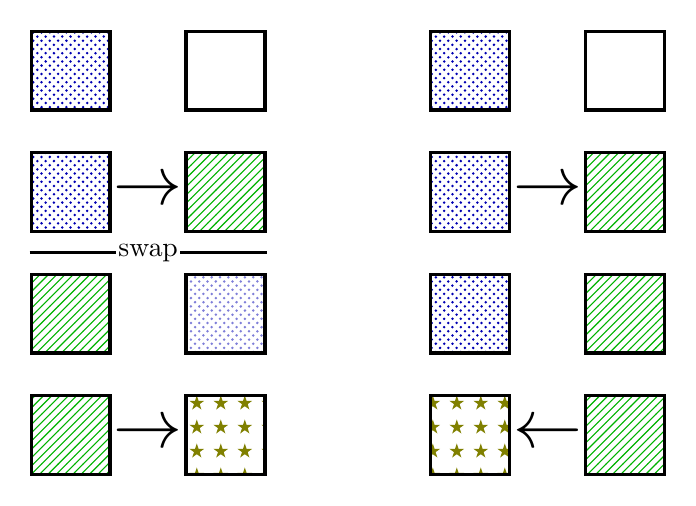
\begin{tikzpicture}
\tikzset{
    grid/.style={anchor=center,draw,very thick,minimum height=1cm,minimum width=1cm},
    grid A/.style={grid,pattern=crosshatch dots,pattern color=blue!70!black},
    grid B/.style={grid,pattern=north east lines,pattern color=green!70!black},
    grid C/.style={grid,pattern=fivepointed stars,pattern color=yellow!50!black},
    faded/.style={fill opacity=0.5},
    for arrow/.style={font=\Huge,anchor=center},
    ampersand replacement=\&,
}
\matrix[row sep=.5cm] (primary) {
    \node[grid A] {}; \& \node[for arrow] {~}; \& \node[grid] (first right) {}; \\
    \node[grid A] (first left) {}; \& \node[for arrow] {$\rightarrow$}; \& \node[grid B] (first right) {}; \\
    \node[grid B] {}; \& \node[for arrow] {~}; \& \node[grid A,faded] {}; \\
    \node[grid B] (second left) {}; \& \node[for arrow] {$\rightarrow$}; \& \node[grid C] (second right) {}; \\
};
    \draw[very thick] ([yshift=-2.5mm]first left.south west) -- ([yshift=-2.5mm]first right.south east)
        node[midway,fill=white]{swap};

\matrix[row sep=.5cm,anchor=north west] (secondary) at ([xshift=2cm]primary.north east) {
    \node[grid A] {}; \& \node[for arrow] {~}; \& \node[grid] {}; \\
    \node[grid A] {}; \& \node[for arrow] {$\rightarrow$}; \& \node[grid B] {}; \\
    \node[grid A] {}; \& \node[for arrow] {~}; \& \node[grid B] {}; \\
    \node[grid C] {}; \& \node[for arrow] {$\leftarrow$}; \& \node[grid B] {}; \\
};
\end{tikzpicture}
\end{frame}


\subsection{x86-64 spinlock}
\begin{frame}[fragile,label=spinlockXchg]{x86-64 spinlock with xchg}
    \begin{itemize}
        \item lock variable in shared memory: \texttt{the\_lock}
        \item if 1: someone has the lock; if 0: lock is free to take
    \end{itemize}
\begin{lstlisting}[
    language=myasm,
    style=smaller,
    morekeywords=mfence,
    moredelim={**[is][\btHL<2|handout:2>]{@2}{2@}},
    moredelim={**[is][\btHL<3|handout:3>]{@3}{3@}},
    moredelim={**[is][\btHL<4|handout:4>]{@4}{4@}},
    moredelim={**[is][\btHL<5|handout:5>]{@5}{5@}},
]
acquire:
    @2movl $1, %eax2@             // %eax <- 1
    @2@5lock5@ xchg %eax, the_lock2@  // swap %eax and the_lock
                                    // sets the_lock to 1 (taken)
                                    // sets %eax to prior val. of the_lock
    @3test %eax, %eax3@           // if the_lock wasn't 0 before:
    @3jne acquire3@               //   try again
    ret

release:
    @5mfence5@                    // for memory order reasons
    @4movl $0, the_lock4@         // then, set the_lock to 0 (not taken)
    ret
\end{lstlisting}
\begin{tikzpicture}[overlay,remember picture]
\coordinate (place) at ([xshift=-1cm,yshift=-1cm]current page.east);
\tikzset{
    box/.style={draw=red,ultra thick,align=left,anchor=east,at={(place)},fill=white},
    box lower/.style={draw=red,ultra thick,align=left,anchor=east,at={(place)},fill=white},
}
\begin{visibleenv}<2>
    \node[box] { set lock variable to 1 (taken) \\ read old value };
\end{visibleenv}
\begin{visibleenv}<3>
    \node[box] { if lock was already locked retry \\ ``spin'' until lock is released elsewhere };
\end{visibleenv}
\begin{visibleenv}<4>
    \node[box] { release lock by setting it to 0 (not taken) \\ allows looping acquire to finish};
\end{visibleenv}
\begin{visibleenv}<5>
    \node[box lower] { Intel's manual says: \\
                 no reordering of loads/stores across a \texttt{lock} \\
                 or \texttt{mfence} instruction
    };
\end{visibleenv}
\end{tikzpicture}
\end{frame}



\subsection{exercise: spin-wait}
\begin{frame}[fragile,label=exerSpinWait]{exercise: spin wait}
\begin{itemize}
\item consider implementing `waiting' functionality of pthread\_join
\vspace{.5cm}
\item thread calls ThreadFinish() when done
\item complete code below:
\end{itemize}
\begin{lstlisting}[language=myasm,style=smaller]
finished: .quad 0
ThreadFinish:
    _________________________
    ret
ThreadWaitForFinish:
    _________________________
    lock xchg %eax, finished
    cmp $0, %eax
    ____ ThreadWaitForFinish
    ret
\end{lstlisting}
\small
\begin{tabular}{lll}
A. \texttt{mfence; mov \$1, finished} & C. \texttt{mov \$0, \%eax} & E. je \\
B. \texttt{mov \$1, finished; mfence} & D. \texttt{mov \$1, \%eax} & F. jne  \\
\end{tabular}
\end{frame}

\begin{frame}<0>[fragile,label=exerSpinWaitSoln]{exercise: spin wait}
\begin{lstlisting}[language=myasm,style=smaller]
finished: .quad 0
ThreadFinish:
    __________A______________
    ret
ThreadWaitForFinish:            /* or without using a writing instruction: */
    _________B______________    mov %eax, finished
    lock xchg %eax, finished    mfence
    cmp $0, %eax                cmp $0, %eax
    __C_ ThreadWaitForFinish    je ThreadWaitForFinish
    ret                         ret
\end{lstlisting}
\small
\begin{tabular}{lll}
A. \texttt{mfence; mov \$1, finished} & C. \texttt{mov \$0, \%eax} & E. je \\
B. \texttt{mov \$1, finished; mfence} & D. \texttt{mov \$1, \%eax} & F. jne  \\
\end{tabular}
\end{frame}
\iftoggle{heldback}{}{\againframe<1>{exerSpinWaitSoln}}


\subsection{spinlock problems}
\begin{frame}<1>[fragile,label=spinLockProblems]{spinlock problems}
    \begin{itemize}
    \item \myemph<4>{lock abstraction is not powerful enough}
        \begin{itemize}
        \item lock/unlock operations don't handle ``wait for event''
        \item common thing we want to do with threads
        \item solution: other synchronization abstractions
        \end{itemize}
    \item \myemph<3>{spinlocks waste CPU time more than needed}
        \begin{itemize}
        \item want to run another thread instead of infinite loop
        \item solution: lock implementation integrated with scheduler
        \end{itemize}
    \item \myemph<2>{spinlocks can send a lot of messages on the shared bus}
        \begin{itemize}
        \item more efficient atomic operations to implement locks
        \end{itemize}
    \end{itemize}
\end{frame}


\subsection{locks that sleep}

\againframe<3>{spinLockProblems}
\begin{frame}{mutexes: intelligent waiting}
\begin{itemize}
    \item want: locks that wait better 
        \begin{itemize}
        \item example: POSIX mutexes
        \end{itemize}
    \item instead of running infinite loop, give away CPU
    \vspace{.5cm}
    \item \myemph<2>{lock = go to sleep}, add self to list
        \begin{itemize}
            \item sleep = scheduler runs something else
        \end{itemize}
    \item \myemph<2>{unlock = wake up sleeping thread}
\end{itemize}
\end{frame}

\begin{frame}{better lock implementation idea}
\begin{itemize}
    \item \textit{shared} list of waiters
    \item \myemph<2>{spinlock protects list of waiters} from concurrent modification
    \vspace{.5cm}
    \item lock = use spinlock to add self to list, then wait without spinlock
    \item unlock = use spinlock to remove item from list
\end{itemize}
\end{frame}



\subsubsection{pseudocode}

\begin{frame}[fragile,label=mutexSketch]{one possible implementation}
\begin{lstlisting}[
    language=C++,
    style=smaller,
    moredelim={**[is][\btHL<2|handout:2>]{@2}{2@}},
    moredelim={**[is][\btHL<3|handout:3>]{@3}{3@}},
    moredelim={**[is][\btHL<4|handout:4>]{@4}{4@}},
    moredelim={**[is][\btHL<5|handout:5>]{@5}{5@}},
]
struct Mutex { 
    @2SpinLock guard_spinlock;2@
    @3bool lock_taken = false;3@
    @4WaitQueue wait_queue;4@
};
\end{lstlisting}
\begin{minipage}{0.45\textwidth}
\begin{lstlisting}[
    language=C++,
    basicstyle=\tt\fontsize{8.5}{9.5}\selectfont,
    moredelim={**[is][\btHL<7-8|handout:7-8>]{@6}{6@}},
]
LockMutex(Mutex *m) {
  LockSpinlock(&m->guard_spinlock);
  if (m->lock_taken) {
    put current thread on m->wait_queue
    mark current thread as waiting
    /* xv6: myproc()->state = SLEEPING; */
    @6UnlockSpinlock(&m->guard_spinlock);6@
    @6run scheduler (context switch)6@
  } else {
    m->lock_taken = true;
    UnlockSpinlock(&m->guard_spinlock);
  }
}
\end{lstlisting}
\end{minipage}
\begin{minipage}{0.45\textwidth}
\begin{lstlisting}[
    language=C++,
    basicstyle=\tt\fontsize{8.5}{9.5}\selectfont,
    moredelim={**[is][\btHL<6|handout:6>]{@5}{5@}},
]
UnlockMutex(Mutex *m) {
  LockSpinlock(&m->guard_spinlock);
  if (m->wait_queue not empty) {
    @5remove a thread from m->wait_queue5@ 
    @5mark thread as no longer waiting5@
    /* xv6: myproc()->state = RUNNABLE; */
  } else {
     m->lock_taken = false;
  }
  UnlockSpinlock(&m->guard_spinlock);
}
\end{lstlisting}
\end{minipage}
\begin{tikzpicture}
\coordinate (header) at ([yshift=-2cm]current page.north west);
\tikzset{
    box/.style={draw=red,thick,fill=white,font=\small,align=left}
}
\begin{visibleenv}<2>
\node[box,anchor=north west] at ([yshift=-1cm]header) {
    spinlock protecting \texttt{lock\_taken} and \texttt{wait\_queue} \\
    only held for very short amount of time (compared to mutex itself)
};
\end{visibleenv}
\begin{visibleenv}<3>
\node[box,anchor=north west] at ([yshift=-1cm]header) {
    tracks whether any thread has locked and not unlocked
};
\end{visibleenv}
\begin{visibleenv}<4>
\node[box,anchor=north west] at ([yshift=-1cm]header) {
    list of threads that discovered lock is taken \\
    and are waiting for it be free \\
    these threads are \myemph{not runnable}
};
\end{visibleenv}
\begin{visibleenv}<6>
\node[box,anchor=north west] at ([yshift=0cm]header) {
    instead of setting lock\_taken to false \\
    choose thread to hand-off lock to
};
\end{visibleenv}
\begin{visibleenv}<7>
\node[box,anchor=north west,fill=white] at ([yshift=0cm]header) {
    subtly: if UnlockMutex runs here on another core\\
    need to make sure scheduler on the other core doesn't switch to thread \\
    while it is still running (would `clone' thread/mess up registers)
};
\end{visibleenv}
\end{tikzpicture}
\end{frame}



\subsubsection{need for scheduler integration}
\begin{frame}{mutex and scheduler subtly}
\small
\begin{tabular}{l|l|l}
core 0 (thread A) & core 1 (thread B) \\ \hline
    start LockMutex & \\
    acquire spinlock & \\
    discover lock taken & \\
    enqueue thread A & \\
    thread A set not runnable & \\
    release spinlock & start UnlockMutex \\
                 & thread A set runnable  \\
                 & finish UnlockMutex \\
                 & run scheduler \\
                 & scheduler switches to A \\
                 & \myemph<2>{\ldots with old verison of registers} \\
    thread A runs scheduler & & \ldots\\
    \ldots finally saving registers & &\ldots\\
\end{tabular}
\begin{itemize}
\item Linux soln.: track `thread running' separately from `thread runnable'
\item xv6 soln.: hold scheduler lock until thread A saves registers 
\end{itemize}
\end{frame}


\subsubsection{analysis: uncontended case}

\begin{frame}{mutex efficiency}
\begin{itemize}
\item `normal' mutex \textbf{\myemph{uncontended}} case:
    \begin{itemize}
    \item lock: acquire + release spinlock, see lock is free
    \item unlock: acquire + release spinlock, see queue is empty
    \end{itemize}
\vspace{.5cm}
\item not much slower than spinlock
\end{itemize}
\end{frame}



\subsection{disabling interrupts for locks}
\begin{frame}{implementing locks: single core}
    \begin{itemize}
    \item intuition: context switch only happens on interrupt
        \begin{itemize}
        \item timer expiration, I/O, etc. causes OS to run
        \end{itemize}
    \item solution: disable them
        \begin{itemize}
        \item reenable on unlock
        \end{itemize}
    \item<2-> x86 instructions:
        \begin{itemize}
        \item \texttt{cli} --- disable interrupts
        \item \texttt{sti} --- enable interrupts
        \end{itemize}
    \end{itemize}
\end{frame}

\begin{frame}[fragile,label=naiveEnableDisable1]{naive interrupt enable/disable (1)}
\begin{tikzpicture}
\node (lock code) {
\begin{lstlisting}[
    language=C++,
    style=small,
    moredelim={**[is][\color{red}\bfseries]{@1}{1@}},
]    
Lock() {
    @1disable interrupts1@
}
\end{lstlisting}
};
\node[anchor=north west] (unlock code) at ([xshift=1cm]lock code.north east) {
\begin{lstlisting}[
    language=C++,
    style=small,
    moredelim={**[is][\color{red}\bfseries]{@1}{1@}},
]    
Unlock() {
    @1enable interrupts1@
}
\end{lstlisting}
};
\end{tikzpicture}
\begin{itemize}
\item<2-> problem: user can \myemph{hang the system}:
\begin{lstlisting}[
    language=C++,
    style=small,
    moredelim={**[is][\btHL<1-|handout:1->]{@1}{1@}},
]    
            Lock(some_lock);
            while (true) {}
\end{lstlisting}
\item<3-> problem: can't do I/O within lock
\begin{lstlisting}[
    language=C++,
    style=small,
    moredelim={**[is][\btHL<1-|handout:1->]{@1}{1@}},
]    
            Lock(some_lock);
            read from disk
                /* waits forever for (disabled) interrupt
                   from disk IO finishing */
\end{lstlisting}
\end{itemize}
\end{frame}


\begin{frame}[fragile,label=naiveEnableDisable2]{naive interrupt enable/disable (2)}
\begin{tikzpicture}
\node (lock code) {
\begin{lstlisting}[
    language=C++,
    style=small,
    moredelim={**[is][\color{red}\bfseries]{@1}{1@}},
]    
Lock() {
    @1disable interrupts1@
}
\end{lstlisting}
};
\node[anchor=north west] (unlock code) at ([xshift=1cm]lock code.north east) {
\begin{lstlisting}[
    language=C++,
    style=small,
    moredelim={**[is][\color{red}\bfseries]{@1}{1@}},
]    
Unlock() {
    @1enable interrupts1@
}
\end{lstlisting}
};
\end{tikzpicture}
\begin{itemize}
\item<4-> problem: nested locks
\begin{lstlisting}[
    language=C++,
    style=small,
    moredelim={**[is][\color{red}\bfseries]{@1}{1@}},
]    
        Lock(milk_lock);
        if (no milk) {
            Lock(store_lock);
            buy milk
            Unlock(store_lock);
            /* interrupts enabled here?? */
        }
        Unlock(milk_lock);
\end{lstlisting}
\end{itemize}
\end{frame}



%\subsection{xv6's push/popcli}
%\begin{frame}[fragile,label=xv6IntDis1]{xv6 interrupt disabling (1)}
\begin{lstlisting}[
    language=C++,
    style=small,
]
...
acquire(struct spinlock *lk) {
  pushcli(); // disable interrupts to avoid deadlock
  ... /* this part basically just for multicore */
}
release(struct spinlock *lk)
{
  ... /* this part basically just for multicore */
  popcli();
}
\end{lstlisting}
\end{frame}

\begin{frame}{xv6 push/popcli}
\begin{itemize}
\item pushcli / popcli --- need to be in pairs
\item pushcli --- disable interrupts if not already
\item popcli --- enable interrupts if corresponding pushcli disabled them
    \begin{itemize}
    \item don't enable them if they were already disabled
    \end{itemize}
\end{itemize}
\end{frame}


\subsection{aside: standard container rules}
\begin{frame}{C++ containers and locking}
    \begin{itemize}
    \item can you use a vector from multiple threads?
    \item \ldots question: how is it implemented?
        \begin{itemize}
        \item<2-> dynamically allocated array
        \item<2-> reallocated on size changes
        \end{itemize}
    \vspace{.5cm}
    \item<3-> can access from multiple threads \ldots \myemph{as long as not append/erase/etc.}?
    \item<3-> assuming it's implemented like we expect\ldots
        \begin{itemize}
        \item but can we really depend on that?
        \item e.g. could shrink internal array after a while with no expansion save memory?
        \end{itemize}
    \end{itemize}
\end{frame}

\begin{frame}[fragile,label=cppStdRules]{C++ standard rules for containers}
\begin{itemize}
    \item multiple threads can \myemph{read anything at the same time}
    \item can only read element \myemph{if no other thread is modifying it}
    \vspace{.5cm}
    \item can safely \myemph{add/remove elements if no other threads} are accessing container
        \begin{itemize}
            \item (sometimes can safely add/remove in extra cases)
        \end{itemize}
    \vspace{.5cm}
    \item exception: vectors of bools --- can't safely read and write at same time
        \begin{itemize}
        \item might be implemented by putting multiple bools in one int
        \end{itemize}
    \end{itemize}
\end{frame}



\subsection{GCC atomic/sync stuff}
\begin{frame}[fragile,label=prevReorder2]{GCC: preventing reordering example (1)}
\begin{lstlisting}[language=C++,style=smaller]
void Alice() {
    int one = 1;
    __atomic_store(&note_from_alice, &one, __ATOMIC_SEQ_CST);
    do {
    } while (__atomic_load_n(&note_from_bob, __ATOMIC_SEQ_CST));
    if (no_milk) {++milk;}
}
\end{lstlisting}
\hrule
\begin{lstlisting}[language=myasm,style=small,morekeywords=mfence]
Alice:
  movl $1, note_from_alice
  mfence
.L2:
  movl note_from_bob, %eax
  testl %eax, %eax
  jne .L2
  ...
\end{lstlisting}
\end{frame}

\begin{frame}[fragile,label=prevReorder1]{GCC: preventing reordering example (2)}
\begin{lstlisting}[language=C++,style=small]
void Alice() {
    note_from_alice = 1;
    do {
        __atomic_thread_fence(__ATOMIC_SEQ_CST);
    } while (note_from_bob);
    if (no_milk) {++milk;}
}
\end{lstlisting}
\hrule
\begin{lstlisting}[language=myasm,style=small,morekeywords=mfence]
Alice:
  movl $1, note_from_alice  // note_from_alice <- 1
.L3:
  mfence  // make sure store is visible to other cores before loading
          // on x86: not needed on second+ iteration of loop
  cmpl $0, note_from_bob  // if (note_from_bob == 0) repeat fence
  jne .L3
  cmpl $0, no_milk
  ...
\end{lstlisting}
\end{frame}




\subsection{exercise: atomic add}
\begin{frame}[fragile,label=atomicOpEx]{exercise: fetch-and-add with compare-and-swap}
\begin{itemize}
\item exercise: implement fetch-and-add with compare-and-swap
\end{itemize}
\begin{lstlisting}[language=C++,style=smaller,deletekeywords=register]
compare_and_swap(address, old_value, new_value) {
    if (memory[address] == old_value) {
        memory[address] = new_value;
        return true;   // x86: set ZF flag
    } else {
        return false;  // x86: clear ZF flag
    }
}
\end{lstlisting}
\end{frame}

\iftoggle{heldback}{
    \excludecomment{heldbackstuff}
}{
    \includecomment{heldbackstuff}
}

\begin{frame}[fragile,label=atomicAdd]{solution}
\begin{heldbackstuff}
\begin{lstlisting}[language=C++,style=smaller,deletekeywords=register]
long my_fetch_and_add(long *p, long amount) {
    long old_value;
    do {
        old_value = *p;
    while (!compare_and_swap(p, old_value, old_value + amount);
    return old_value;
}
\end{lstlisting}
\end{heldbackstuff}
\end{frame}

\subsection{xv6's spinlock debugging}

\begin{frame}[fragile,label=xv6SpinlockAcquire]{xv6 spinlock: acquire}
\begin{lstlisting}[
    language=C++,
    style=smaller,
    morekeywords=mfence,
    moredelim={**[is][\btHL<2|handout:2>]{@2}{2@}},
    moredelim={**[is][\btHL<3|handout:3>]{@3}{3@}},
    moredelim={**[is][\btHL<4|handout:4>]{@4}{4@}},
    moredelim={**[is][\btHL<5|handout:5>]{@5}{5@}},
]
void
acquire(struct spinlock *lk)
{
  @2pushcli();2@ // disable interrupts to avoid deadlock.
  ...
  // The xchg is atomic.
  @3while(xchg(&lk->locked, 1) != 0)3@
    ; 

  // Tell the C compiler and the processor to not move loads or stores
  // past this point, to ensure that the critical section's memory
  // references happen after the lock is acquired.
  @4__sync_synchronize();4@
  ...
}
\end{lstlisting}
\begin{tikzpicture}[overlay,remember picture]
\coordinate (place) at ([yshift=1cm]current page.south);
\coordinate (place higher) at ([yshift=3cm]current page.south);
\tikzset{
    box/.style={draw=red,ultra thick,fill=white,align=left,at={(place)},anchor=south},
    box higher/.style={draw=red,ultra thick,fill=white,align=left,at={(place higher)},anchor=south},
}
\begin{visibleenv}<2>
    \node[box] {
        don't let us be interrupted after while have the lock \\
        problem: interruption might try to do something with the lock \\
        \ldots but that can never succeed until we release the lock \\
        \ldots but we won't release the lock until interruption finishes
    };
\end{visibleenv}
\begin{visibleenv}<3>
    \node[box] {
        xchg wraps the lock xchg instruction \\
        same loop as before
    };
\end{visibleenv}
\begin{visibleenv}<4>
    \node[box] {
        avoid load store reordering (including by compiler) \\
        on x86, \texttt{xchg} alone is enough to avoid processor's reordering \\
        (but compiler may need more hints)
    };
\end{visibleenv}
\end{tikzpicture}
\end{frame}

\begin{frame}[fragile,label=xv6SpinlockRelease]{xv6 spinlock: release}
\begin{lstlisting}[
    language=C++,
    style=smaller,
    morekeywords=mfence,
    moredelim={**[is][\btHL<2|handout:2>]{@2}{2@}},
    moredelim={**[is][\btHL<3|handout:3>]{@3}{3@}},
    moredelim={**[is][\btHL<4|handout:4>]{@4}{4@}},
    moredelim={**[is][\btHL<5|handout:5>]{@5}{5@}},
]
void
release(struct spinlock *lk)
  ...
  // Tell the C compiler and the processor to not move loads or stores
  // past this point, to ensure that all the stores in the critical
  // section are visible to other cores before the lock is released.
  // Both the C compiler and the hardware may re-order loads and
  // stores; __sync_synchronize() tells them both not to.
  @2__sync_synchronize();2@

  // Release the lock, equivalent to lk->locked = 0.
  // This code can't use a C assignment, since it might
  // not be atomic. A real OS would use C atomics here.
  @3asm volatile("movl $0, %0" : "+m" (lk->locked) : );3@

  @4popcli();4@
}
\end{lstlisting}
\begin{tikzpicture}[overlay,remember picture]
\coordinate (place) at ([yshift=1cm]current page.south);
\tikzset{
    box/.style={draw=red,ultra thick,fill=white,align=left,at={(place)},anchor=south},
}
\begin{visibleenv}<2>
    \node[box] {
        turns into instruction to tell processor not to reorder \\
        plus tells compiler not to reorder
    };
\end{visibleenv}
\begin{visibleenv}<3>
    \node[box] {
        turns into mov of constant 0 into \lstinline|lk->locked|
    };
\end{visibleenv}
\begin{visibleenv}<4>
    \node[box] {
        reenable interrupts (taking nested locks into account)
    };
\end{visibleenv}
\end{tikzpicture}
\end{frame}


\subsection{CAS for fetch-and-add}
\begin{frame}[fragile,label=fetchAndAddWithCASSetup]{fetch-and-add with CAS (1)}
\begin{lstlisting}[language=C++,style=smaller,deletekeywords=register]
compare-and-swap(address, old_value, new_value) {
    if (memory[address] == old_value) {
        memory[address] = new_value;
        return true;
    } else {
        return false;
    }
}
\end{lstlisting}
\hrule
\begin{lstlisting}[language=C++,style=smaller,deletekeywords=register]
long my_fetch_and_add(long *pointer, long amount) { ... }
\end{lstlisting}
    \begin{itemize}
    \item implementation sketch:
        \begin{itemize}
        \item fetch value from pointer \texttt{old}
        \item compute in temporary value result of addition \texttt{new}
        \item try to change value at pointer from \texttt{old} to \texttt{new} [\texttt{compare-and-swap}]
        \item if not successful, repeat
        \end{itemize}
    \end{itemize}
\end{frame}

\begin{frame}[fragile,label=fetchAndAddWithCASSoln]{fetch-and-add with CAS (2)}
\begin{lstlisting}[language=C++,style=smaller,deletekeywords=register]
long my_fetch_and_add(long *p, long amount) {
    long old_value;
    do {
        old_value = *p;
    } while (!compare_and_swap(p, old_value, old_value + amount);
    return old_value;
}
\end{lstlisting}
\end{frame}



\subsection{exercise: CAS for appending to list}
\begin{frame}[fragile,label=appendToListExercise]{exercise: append to singly-linked list}
\begin{itemize}
    \item ListNode is a singly-linked list
    \item assume: threads \textit{only} append to list (no deletions, reordering)
    \item use \texttt{compare-and-swap(pointer, old, new)}:
        \begin{itemize}
        \item atomically change \texttt{*pointer} from \texttt{old} to \texttt{new}
        \item return true if successful
        \item return false (and change nothing) if \texttt{*pointer} is not \texttt{old}
        \end{itemize}
\end{itemize}
\begin{lstlisting}[language=C++,style=smaller]
void append_to_list(ListNode *head, ListNode *new_last_node) {
    ...
}
\end{lstlisting}
\end{frame}

\begin{frame}<0>[fragile,label=appendToListSol]{append to singly-linked list}
\begin{lstlisting}[language=C++,style=smaller]
/* assumption: other threads may be appending to list,
 *             but nodes are not being removed, reordered, etc.
 */
void append_to_list(ListNode *head, ListNode *new_last_node) {
  memory_ordering_fence();
  ListNode *current_last_node;
  do {
    current_last_node = head;
    while (current_last_node->next) {
      current_last_node = current_last_node->next;
    }
  } while (
    !compare-and-swap(&current_last_node->next,
                      NULL, new_last_node)
  );
}
\end{lstlisting}
\end{frame}

\iftoggle{heldback}{}{\againframe<1>{appendToListSol}}


\subsection{more atomic operations}


\begin{frame}[fragile,label=moreCommonAtomic1]{some common atomic operations (1)}
\begin{lstlisting}[language=C++,style=smaller,deletekeywords=register]
// x86: emulate with exchange
test_and_set(address) {
    old_value = memory[address];
    memory[address] = 1;
    return old_value != 0;  // e.g. set ZF flag
}

// x86: xchg REGISTER, (ADDRESS)
exchange(register, address) {
    temp = memory[address];
    memory[address] = register;
    register = temp;
}
\end{lstlisting}
\end{frame}

\begin{frame}[fragile,label=moreCommonAtomic2]{some common atomic operations (2)}
\begin{lstlisting}[language=C++,style=smaller,deletekeywords=register]
// x86: mov OLD_VALUE, %eax; lock cmpxchg NEW_VALUE, (ADDRESS)
compare-and-swap(address, old_value, new_value) {
    if (memory[address] == old_value) {
        memory[address] = new_value;
        return true;   // x86: set ZF flag
    } else {
        return false;  // x86: clear ZF flag
    }
}

// x86: lock xaddl REGISTER, (ADDRESS)
fetch-and-add(address, register) {
    old_value = memory[address];
    memory[address] += register;
    register = old_value;
}
\end{lstlisting}
\end{frame}

\begin{frame}{common atomic operation pattern}
    \begin{itemize}
    \item try to do operation, \ldots
    \item detect if it failed
    \item if so, repeat
    \vspace{.5cm}
    \item atomic operation does ``try and see if it failed'' part
    \end{itemize}
\end{frame}





\subsection{cache coherency detail}
\subsection{adding more state: MSI}
\usetikzlibrary{arrows.meta,matrix,positioning,shapes.callouts}

\begin{frame}{cache coherency states}
\begin{itemize}
\item extra information for \myemph{each cache block}
    \begin{itemize}
        \item overlaps with/replaces valid, dirty bits
    \end{itemize}
\item stored in \myemph{each cache}
\item update states based on reads, writes \myemph{and heard messages on bus}
\item different caches may have different states for same block
\end{itemize}
\end{frame}

\begin{frame}{MSI state summary}
\begin{tabular}{lp{10cm}}
{\bfseries Modified} & {value may be \myemph{different than memory} \textit{and} I am the only one who has it } \\
~ & ~ \\
{\bfseries Shared} & value is the \myemph{same as memory} \\
~ & ~ \\
{\bfseries Invalid} & I don't have the value; I will need to ask for it \\
\end{tabular}
\end{frame}

\begin{frame}{MSI scheme}
\begin{tabular}{lllll}
from state & hear read & hear write & read & write \\ \hline
Invalid & --- & --- & \color{blue}to Shared & \color{blue}to Modified \\
Shared & --- & to Invalid & --- & \color{blue}to Modified \\
Modified & \color{blue}to Shared & \color{blue}to Invalid & --- & --- \\
\end{tabular}
\begin{itemize}
\item {\color{blue}blue}: transition requires sending message on bus
\item<2-> example: write while Shared 
    \begin{itemize}
    \item must send write --- inform others with Shared state
    \item then change to Modified
    \end{itemize}
\item<3-> example: hear write while Shared
    \begin{itemize}
    \item change to Invalid
    \item can send read later to get value from writer
    \end{itemize}
\item<3-> example: write while Modified
    \begin{itemize}
    \item nothing to do --- no other CPU can have a copy
    \end{itemize}
\end{itemize}
\end{frame}

\begin{frame}[fragile,label=msiExample]{MSI example}
\begin{tikzpicture}
\matrix[
    matrix of nodes,
    nodes in empty cells,
    row 1/.style={nodes={minimum height=1cm,minimum width=1cm}},
    row 2/.style={nodes={draw,rectangle,minimum height=1cm,minimum width=1cm}},
    column sep=2.75cm,
] (net) {
      \& \& \\
    CPU1 \& CPU2 \& MEM1 \\
};
\foreach \x in {1,2,3} {
    \draw[thick] (net-2-\x.north) -- (net-1-\x.center);
}
\draw[thick,Latex-Latex] (net-1-1.west) -- (net-1-3.east);
\tikzset{
    cache/.style={
        tight matrix,
        nodes={font=\small\ttfamily,text width=1.8cm,execute at begin node={\strut}},
        row 1/.append style={nodes={font=\small\bfseries}},
        column 3/.append style={nodes={font=\sffamily\small}},
    },
}
\matrix[cache,anchor=north] (cache1) at (net-2-1.south east){
    address \& value \& state\\
    0xA300 \& \only<1-2>{\sout<2->{100}}\only<2-3>{\sout<3->{\myemph<2>{101}}}\only<3->{\myemph<3,5>{102}} 
           \& \only<1>{Shared}\only<2-4>{\myemph<2>{Modified}}\only<5->{\myemph<5>{Shared}}\\
    0xC400 \& 200 \& Shared\\
    0xE500 \& 300 \& Shared \\
};
\matrix[cache,anchor=north] (cache2) at ([xshift=1.5cm]net-2-2.south east){
    address \& value \& state\\
    0x9300 \& 172 \& Shared \\ 
    \sout<2->{0xA300} \& \sout<2->{100}\only<6->{\myemph<6>{102}} \& \only<1>{Shared}\only<2-5>{\myemph<2>{Invalid}}\only<6>{\myemph<6>{Shared}} \\
    0xC500 \& 200 \& Shared\\
};
\begin{visibleenv}<2>
    \draw[blue,very thick,-Latex]  (net-2-1.north) -- (net-1-1.center) 
        node[above,xshift=2cm] {``CPU1 is writing 0xA3000''} -- (net-1-2.center) --(net-2-2.north);
    \draw[blue,dashed,very thick,-Latex]  (net-2-1.north) -- (net-1-1.center) -- (net-1-3.center) --(net-2-3.north);
\node[draw,thick,draw=blue,rectangle,anchor=north west] at ([yshift=-1cm]cache1.south west){
    CPU1 writes 101 to 0xA300
};
\node[my callout2=cache2-3-2,anchor=north,align=left] at ([yshift=-.5cm]cache2-3-2.south) {
    cache sees write: \\ invalidate 0xA300
};
\node[my callout2=net-2-3.center,anchor=south] at ([yshift=1.5cm,xshift=-1.5cm]net-2-3.center) {
    maybe update memory?
};
\end{visibleenv}
\begin{visibleenv}<3>
\node[draw,thick,draw=blue,rectangle,anchor=north west] (writeTo) at ([yshift=-1cm]cache1.south west){
    CPU1 writes 102 to 0xA300
};
\node[my callout2=cache1-2-3,anchor=north,align=left] at ([xshift=2cm,yshift=-.5cm]cache1-2-2.south) {
    modified state --- nothing communicated! \\
    will ``fix'' later if there's a read
};
\node[my callout2=net-2-3.center,anchor=south] at ([yshift=1.5cm,xshift=-2cm]net-2-3.center) {
    nothing changed yet (\myemph{writeback})
};
\end{visibleenv}
\begin{visibleenv}<4>
    \draw[blue,dashed,very thick,-Latex]  (net-2-2.north) -- (net-1-2.center) -- (net-1-1.center) --(net-2-1.north);
    \draw[blue,very thick,-Latex]  (net-2-2.north) -- (net-1-2.center) node[above] {``What is 0xA300?''} -- (net-1-3.center) --(net-2-3.north);
\node[draw,thick,draw=blue,rectangle,anchor=north west] at ([yshift=-1cm]cache2.south west){
    CPU2 reads 0xA300
};
\node[my callout2=cache1-2-2,anchor=north] at ([yshift=-.5cm]cache1-2-3.south) {
    modified state --- must update for CPU2!
};
\end{visibleenv}
\begin{visibleenv}<5>
    \draw[blue,dashed,very thick,-Latex]  (net-2-1.north) -- (net-1-1.center) -- (net-1-3.center) --(net-2-3.north);
    \draw[blue,very thick,-Latex]  (net-2-1.north) -- (net-1-1.center) node[above,xshift=1cm] {``Write 102 into 0xA300''} -- (net-1-3.center) --(net-2-3.north);
\node[draw,thick,draw=blue,rectangle,anchor=north west] at ([yshift=-1cm]cache2.south west){
    CPU2 reads 0xA300
};
\node[my callout2=cache1-2-2,anchor=north,align=left] at ([yshift=-.5cm]cache1-2-3.south) {
    written back to memory early \\
    (could also become Invalid at CPU1)
};
\end{visibleenv}
\end{tikzpicture}
\end{frame}

\begin{frame}{MSI: update memory}
\begin{itemize}
    \item to write value (enter modified state), need to \myemph{invalidate} others
    \item can avoid sending actual value (shorter message/faster)
    \vspace{.5cm}
    \item ``I am writing address $X$'' versus ``I am writing $Y$ to address $X$''
\end{itemize}
\end{frame}

\begin{frame}{MSI: on cache replacement/writeback}
\begin{itemize}
    \item still happens --- e.g. want to store something else
    \item changes state to \myemph{invalid}
    \item requires writeback if modified (= dirty bit)
\end{itemize}
\end{frame}




\subsection{exercise}
\begin{frame}{cache coherency exercise}
\begin{itemize}
\item modified/shared/invalid; all initially invalid; 32B blocks, 8B read/writes
\begin{itemize}
\item CPU 1: read 0x1000
\item CPU 2: read 0x1000
\item CPU 1: write 0x1000
\item CPU 1: read 0x2000
\item CPU 2: read 0x1000
\item CPU 2: write 0x2008
\item CPU 3: read 0x1008
\end{itemize}
\item Q1: final state of 0x1000 in caches? 
    \begin{itemize}
    \item Modified/Shared/Invalid for CPU 1/2/3
    \item CPU 1: \hspace{2cm} CPU 2: \hspace{2cm} CPU 3: \hspace{2cm}
    \end{itemize}
\item Q2: final state of 0x2000 in caches? 
    \begin{itemize}
    \item Modified/Shared/Invalid for CPU 1/2/3
    \item CPU 1: \hspace{2cm} CPU 2: \hspace{2cm} CPU 3: \hspace{2cm}
    \end{itemize}
\end{itemize}
\end{frame}

\begin{frame}<0>[label=cacheCoherenceExSoln]{cache coherency exercise solution}
\tt
\begin{tabular}{l|ccc|ccc}
~ & \multicolumn{3}{c|}{\tt 0x1000-0x101f} & \multicolumn{3}{c}{\tt 0x2000-0x201f} \\
\normalfont\bfseries action & \normalfont CPU 1 & \normalfont CPU 2 & \normalfont CPU 3 & \normalfont CPU 1 & \normalfont CPU 2 & \normalfont CPU 3 \\ \hline
~   & I & I & I & I & I & I \\
\normalfont CPU 1: read \tt 0x1000
    & \myemph{S} & I & I & I & I & I \\
\normalfont CPU 2: read \tt 0x1000
    & S & \myemph{S} & I & I & I & I \\
\normalfont CPU 1: write \tt 0x1000
    & \myemph{M} & \myemph{I} & I & I & I & I \\
\normalfont CPU 1: read \tt 0x2000
    & M & I & I & \myemph{S} & I & I \\
\normalfont CPU 2: read \tt 0x1000 
    & \myemph{S} & \myemph{S} & I & S & I & I \\
\normalfont CPU 2: write \tt 0x2008
    & S & S & I & \myemph{I} & \myemph{M} & I \\
\normalfont CPU 3: read \tt 0x1008
    & S & S & \myemph{S} & I & M & I \\
\end{tabular}
%\item CPU 1: read 0x1000
%\item CPU 2: read 0x1000
%\item CPU 1: write 0x1000
%\item CPU 1: read 0x2000
%\item CPU 2: read 0x1000
%\item CPU 2: write 0x2008
%\item CPU 3: read 0x1008
\end{frame}

\iftoggle{heldback}{}{
    \againframe<1->{cacheCoherenceExSoln}
}


\section{processor load/store reordering}
% FIXME: instruction queue/etc. picture?
\usetikzlibrary{calc}

\begin{frame}{why load/store reordering?}
\begin{itemize}
\item fast processor designs can execute instructions out of order
\item goal: do something instead of waiting for slow memory accesses, etc.
\item more on this later in the semester
\end{itemize}
\end{frame}



\subsection{C++atomic/sync stuff}


\begin{frame}{C++: preventing reordering}
    \begin{itemize}
        \item to help \myemph{implementing things like pthread\_mutex\_lock}
        \vspace{.5cm}
    \item C++ 2011 standard: \textit{atomic} header, \textit{std::atomic} class
        \item prevent CPU reordering \textit{and} prevent compiler reordering
        \item also provide other tools for implementing locks (more later)
            \vspace{.5cm}
        \item could also hand-write assembly code
            \begin{itemize}
                \item compiler can't know what assembly code is doing
            \end{itemize}
    \end{itemize}
\end{frame}

\begin{frame}[fragile,label=prevReorderCpp1]{C++: preventing reordering example}
\begin{lstlisting}[language=C++,style=smaller]
#include <atomic>
void Alice() {
    note_from_alice = 1;
    do {
        std::atomic_thread_fence(std::memory_order_seq_cst);
    } while (note_from_bob);
    if (no_milk) {++milk;}
}
\end{lstlisting}
\hrule
\begin{lstlisting}[language=myasm,style=smaller,morekeywords=mfence]
Alice:
  movl $1, note_from_alice  // note_from_alice <- 1
.L2:
  mfence  // make sure store visible on/from other cores
  cmpl $0, note_from_bob  // if (note_from_bob == 0) repeat fence
  jne .L2
  cmpl $0, no_milk
  ...
\end{lstlisting}
\end{frame}

\begin{frame}[fragile,label=prevReorderCpp2]{C++ atomics: no reordering}
\begin{lstlisting}[language=C++,style=smaller]
std::atomic<int> note_from_alice, note_from_bob;
void Alice() {
    note_from_alice.store(1);
    do {
    } while (note_from_bob.load());
    if (no_milk) {++milk;}
}
\end{lstlisting}
\hrule
\begin{lstlisting}[language=myasm,style=small,morekeywords=mfence]
Alice:
  movl $1, note_from_alice
  mfence
.L2:
  movl note_from_bob, %eax
  testl %eax, %eax
  jne .L2
  ...
\end{lstlisting}
\end{frame}
\begin{frame}{GCC: built-in atomic functions}
    \begin{itemize}
    \item used to implement std::atomic, etc.
    \item predate std::atomic
        \vspace{.5cm}
    \item builtin functions starting with \texttt{\_\_sync} and \texttt{\_\_atomic}
    \item these are what xv6 uses
    \end{itemize}
\end{frame}



\subsection{x86-64 reordering rules}

\begin{frame}{aside: some x86 reordering rules}
\begin{itemize}
\item each core sees its own loads/stores in order
    \begin{itemize}
    \item (if a core stores something, it can always load it back)
    \end{itemize}
\item stores \textit{from other cores} appear in a consistent order
    \begin{itemize}
    \item (but a core might observe its own stores too early)
    \end{itemize}
\item \textit{causality}: \\
    \textit{if} a core reads X=a and (after reading X=a) writes Y=b, \\
    \textit{then} a core that reads Y=b cannot later read X=older value than a
\end{itemize}
\imagecredit{Source: Intel 64 and IA-32 Software Developer's Manual, Volume 3A, Chapter 8}
\end{frame}

\begin{frame}{how do you do anything with this?}
    \begin{itemize}
    \item difficult to reason about what modern CPU's reordering rules do
    \item typically: don't depend on details, instead:
    \vspace{.5cm}
    \item special instructions with stronger (and simpler) ordering rules
        \begin{itemize}
        \item often same instructions that help with implementing locks in other ways
        \end{itemize}
    \item special instructions that restrict ordering of instructions around them (``fences'')
        \begin{itemize}
        \item loads/stores can't cross the fence
        \end{itemize}
    \end{itemize}
\end{frame}




\subsection{test-and-test-and-set}

\againframe<2>{spinLockProblems}
% FIXME: what 3 CPUs, ping-pong between CPU2 and CPU3
\usetikzlibrary{arrows.meta,matrix,positioning,shapes.callouts}

\begin{frame}{ping-ponging}
\begin{tikzpicture}
\matrix[
    matrix of nodes,
    nodes in empty cells,
    row 1/.style={nodes={minimum height=1cm,minimum width=1cm}},
    row 2/.style={nodes={draw,rectangle,minimum height=1cm,minimum width=1cm}},
    column sep=2.75cm,
] (net) {
    \& \& \& \\
    CPU1 \& CPU2 \& CPU3 \& MEM1 \\
};
\foreach \x in {1,2,3,4} {
    \draw[thick] (net-2-\x.north) -- (net-1-\x.center);
}
\draw[thick,Latex-Latex] (net-1-1.west) -- (net-1-4.east);
\tikzset{
    cache/.style={
        tight matrix,
        nodes={font=\fontsize{9}{10}\ttfamily\selectfont,text width=1.5cm,execute at begin node={\strut}},
        row 1/.append style={nodes={font=\fontsize{9}{10}\bfseries\selectfont}},
        column 3/.append style={nodes={font=\fontsize{9}{10}\sffamily\selectfont}},
    },
}
\matrix[cache,anchor=north] (cache1) at (net-2-1.south east){
    address \& value \& state\\
    lock \& \only<1>{locked}\only<2-5,7>{\myemph<2,7>{---}}\only<6>{\myemph<6>{unlocked}} \& \only<1,6>{Modified}\only<2-5,7>{\myemph{Invalid}} \\
};
\matrix[cache,anchor=north] (cache2) at ([xshift=.75cm]net-2-2.south east){
    address \& value \& state\\
    lock \& \only<1,3,5-6>{---}\only<2,4,7>{\myemph{locked}} \& \only<1,3,5,6>{\myemph<2,4>{Invalid}}\only<2,4,7>{\myemph{Modified}} \\
};
\matrix[cache,anchor=north] (cache3) at ([xshift=1.5cm]net-2-3.south east){
    address \& value \& state\\
    lock \& \only<1-2,4>{---}\only<3,5>{\myemph{locked}} \& \only<1-2,4,6-7>{\myemph<4>{Invalid}}\only<3,5>{\myemph{Modified}} \\
};
\begin{visibleenv}<2,4>
    \draw[blue,dashed,very thick,-Latex]  (net-2-2.north) -- (net-1-2.center) -- (net-1-1.center) --(net-2-1.north);
    \draw[blue,very thick,-Latex]  (net-2-2.north) -- (net-1-2.center) node[above] {``I want to modify \texttt{lock}?''} -- (net-1-4.center) --(net-2-4.north);
\node[align=center,draw,thick,draw=blue,rectangle,anchor=north west] at ([yshift=-1cm]cache1.south west){
    CPU2 read-modify-writes lock \\ (to see it is still locked)
};
\end{visibleenv}
\begin{visibleenv}<3,5>
    \draw[blue,dashed,very thick,-Latex]  (net-2-3.north) -- (net-1-3.center) -- (net-1-4.center) --(net-2-4.north);
    \draw[blue,very thick,-Latex]  (net-2-3.north) -- (net-1-3.center) node[above,xshift=1cm] {``I want to modify \texttt{lock}''} -- (net-1-2.center) --(net-2-2.north);
\node[align=center,draw,thick,draw=blue,rectangle,anchor=north west] at ([yshift=-1cm]cache1.south west){
    CPU3 read-modify-writes lock \\ (to see it is still locked)
};
\end{visibleenv}
\begin{visibleenv}<6>
    \draw[blue,dashed,very thick,-Latex]  (net-2-1.north) -- (net-1-1.center) -- (net-1-4.center) --(net-2-4.north);
    \draw[blue,very thick,-Latex]  (net-2-1.north) -- (net-1-1.center) node[above,xshift=1cm] {``I want to modify \texttt{lock}''} -- (net-1-3.center) --(net-2-3.north);
\node[align=center,draw,thick,draw=blue,rectangle,anchor=north west] at ([yshift=-1cm]cache1.south west){
    CPU1 sets lock to unlocked
};
\end{visibleenv}
\begin{visibleenv}<7>
    \draw[blue,dashed,very thick,-Latex]  (net-2-1.north) -- (net-1-1.center) -- (net-1-4.center) --(net-2-4.north);
    \draw[blue,very thick,-Latex]  (net-2-1.north) -- (net-1-1.center) node[above,xshift=1cm] {``I want to modify \texttt{lock}''} -- (net-1-3.center) --(net-2-3.north);
\node[align=center,draw,thick,draw=blue,rectangle,anchor=north west] at ([yshift=-1cm]cache1.south west){
    some CPU (this example: CPU2) acquires lock
};
\end{visibleenv}
\end{tikzpicture}
\end{frame}

\begin{frame}{ping-ponging}
    \begin{itemize}
    \item test-and-set problem: cache block ``ping-pongs'' between caches
        \begin{itemize}
        \item each waiting processor reserves block to modify
        \item could maybe wait until it determines modification needed --- but not typical implementation
        \end{itemize}
    \item each transfer of block sends messages on bus
    \item \ldots so bus can't be used for real work
        \begin{itemize}
        \item like what the processor with the lock is doing
        \end{itemize}
    \end{itemize}
\end{frame}

\begin{frame}[fragile,label=testAndTestAndSetC]{test-and-test-and-set (pseudo-C)}
\begin{lstlisting}[language=C,style=smaller]
acquire(int *the_lock) {
    do {
        while (ATOMIC-READ(the_lock) == 0) { /* try again */ }
    } while (ATOMIC-TEST-AND-SET(the_lock) == ALREADY_SET);
}
\end{lstlisting}
\end{frame}

\begin{frame}[fragile,label=testAndTestAndSetASM]{test-and-test-and-set (assembly)}
\begin{lstlisting}[language=myasm,style=smaller]
acquire:
    cmp $0, the_lock         // test the lock non-atomically
            // unlike lock xchg --- keeps lock in Shared state!
    jne acquire              // try again (still locked)
    // lock possibly free
    // but another processor might lock
    // before we get a chance to
    // ... so try wtih atomic swap:
    movl $1, %eax             // %eax <- 1
    lock xchg %eax, the_lock  // swap %eax and the_lock
           // sets the_lock to 1
           // sets %eax to prior value of the_lock
    test %eax, %eax           // if the_lock wasn't 0 (someone else got it first):
    jne acquire               //   try again
    ret
\end{lstlisting}
\end{frame}

\begin{frame}{less ping-ponging}
\begin{tikzpicture}
\matrix[
    matrix of nodes,
    nodes in empty cells,
    row 1/.style={nodes={minimum height=1cm,minimum width=1cm}},
    row 2/.style={nodes={draw,rectangle,minimum height=1cm,minimum width=1cm}},
    column sep=2.75cm,
] (net) {
    \& \& \& \\
    CPU1 \& CPU2 \& CPU3 \& MEM1 \\
};
\foreach \x in {1,2,3,4} {
    \draw[thick] (net-2-\x.north) -- (net-1-\x.center);
}
\draw[thick,Latex-Latex] (net-1-1.west) -- (net-1-4.east);
\tikzset{
    cache/.style={
        tight matrix,
        nodes={font=\fontsize{9}{10}\ttfamily\selectfont,text width=1.5cm,execute at begin node={\strut}},
        row 1/.append style={nodes={font=\fontsize{9}{10}\bfseries\selectfont}},
        column 3/.append style={nodes={font=\fontsize{9}{10}\sffamily\selectfont}},
    },
}
\matrix[cache,anchor=north] (cache1) at (net-2-1.south east){
    address \& value \& state\\
    lock \& \only<1-5>{locked}\only<6>{\myemph<6>{unlocked}} \& \only<1-2,6->{\myemph{Modified}}\only<3-5>{\myemph<3>{Shared}} \\
};
\matrix[cache,anchor=north] (cache2) at ([xshift=.75cm]net-2-2.south east){
    address \& value \& state\\
    lock \& \only<1,6>{---}\only<3-5>{\myemph<3,5>{locked}} \& \only<1-2>{Invalid}\only<3-5>{\myemph<3>{Shared}}\only<6->{\myemph<6>{Invalid}} \\
};
\matrix[cache,anchor=north] (cache3) at ([xshift=1.5cm]net-2-3.south east){
    address \& value \& state\\
    lock \& \only<1,6>{---}\only<4-5>{\myemph<4,5>{locked}} \& \only<1-3>{Invalid}\only<4-5>{\myemph<4>{Shared}}\only<6->{\myemph<6>{Invalid}} \\
};
\begin{visibleenv}<2>
    \draw[blue,dashed,very thick,-Latex]  (net-2-2.north) -- (net-1-2.center) -- (net-1-1.center) --(net-2-1.north);
    \draw[blue,very thick,-Latex]  (net-2-2.north) -- (net-1-2.center) node[above] {``I want to read \texttt{lock}?''} -- (net-1-4.center) --(net-2-4.north);
\node[align=center,draw,thick,draw=blue,rectangle,anchor=north west] at ([yshift=-1cm]cache1.south west){
    CPU2 reads lock \\ (to see it is still locked)
};
\end{visibleenv}
\begin{visibleenv}<3>
    \draw[blue,dashed,very thick,-Latex]  (net-2-2.north) -- (net-1-2.center) -- (net-1-1.center) --(net-2-1.north);
    \draw[blue,very thick,-Latex]  (net-2-1.north) -- (net-1-1.center) node[above] {``set lock to locked''} -- (net-1-4.center) --(net-2-4.north);
\node[align=center,draw,thick,draw=blue,rectangle,anchor=north west] at ([yshift=-1cm]cache1.south west){
    CPU1 writes back lock value, \\ then CPU2 reads it
};
\end{visibleenv}
\begin{visibleenv}<4>
    \draw[blue,dashed,very thick,-Latex]  (net-2-3.north) -- (net-1-3.center) -- (net-1-4.center) --(net-2-4.north);
    \draw[blue,very thick,-Latex]  (net-2-3.north) -- (net-1-3.center) node[above,xshift=1cm] {``I want to read \texttt{lock}''} -- (net-1-4.center) --(net-2-4.north);
\node[align=center,draw,thick,draw=blue,rectangle,anchor=north west] at ([yshift=-1cm]cache1.south west){
    CPU3 reads lock \\ (to see it is still locked)
};
\end{visibleenv}
\begin{visibleenv}<5>
\node[align=center,draw,thick,draw=blue,rectangle,anchor=north west] at ([yshift=-1cm]cache1.south west){
    CPU2, CPU3 continue to read lock from cache \\
    no messages on the bus
};
\end{visibleenv}
\begin{visibleenv}<6>
    \draw[blue,dashed,very thick,-Latex]  (net-2-1.north) -- (net-1-1.center) -- (net-1-4.center) --(net-2-4.north);
    \draw[blue,very thick,-Latex]  (net-2-1.north) -- (net-1-1.center) node[above,xshift=1cm] {``I want to modify \texttt{lock}''} -- (net-1-3.center) --(net-2-3.north);
\node[align=center,draw,thick,draw=blue,rectangle,anchor=north west] at ([yshift=-1cm]cache1.south west){
    CPU1 sets lock to unlocked
};
\end{visibleenv}
\begin{visibleenv}<7>
    \draw[blue,dashed,very thick,-Latex]  (net-2-1.north) -- (net-1-1.center) -- (net-1-4.center) --(net-2-4.north);
    \draw[blue,very thick,-Latex]  (net-2-1.north) -- (net-1-1.center) node[above,xshift=1cm] {``I want to modify \texttt{lock}''} -- (net-1-3.center) --(net-2-3.north);
\node[align=center,draw,thick,draw=blue,rectangle,anchor=north west] at ([yshift=-1cm]cache1.south west){
    some CPU (this example: CPU2) acquires lock \\
    (CPU1 writes back value, then CPU2 reads + modifies it)
};
\end{visibleenv}
\end{tikzpicture}
\end{frame}

\begin{frame}{couldn't the read-modify-write instruction\ldots}
    \begin{itemize}
    \item notice that the value of the lock isn't changing\ldots
    \item and keep it in the shared state
        \vspace{.5cm}
    \item maybe --- but extra step in ``common'' case \\ (swapping different values)
    \end{itemize}
\end{frame}

\begin{frame}{more room for improvement?}
    \begin{itemize}
    \item can still have a lot of attempts to modify locks after unlocked
    \item there other spinlock designs that avoid this
        \begin{itemize}
        \item ticket locks
        \item MCS locks
        \item \ldots
        \end{itemize}
    \end{itemize}
\end{frame}



\subsection{beyond MSI}
\begin{frame}{MSI extensions}
\begin{itemize}
\item real cache coherency protocols sometimes more complex:
\vspace{.5cm}
\item separate tracking modifications from whether other caches have copy
\item send values directly between caches (maybe skip write to memory)
\item send messages only to cores which might care (no shared bus)
\end{itemize}
\end{frame}


\section{relating monitors and semaphores}

\subsection{implementing monitors with semaphores}

\begin{frame}[fragile,label=monitorWithSemaphoreLock]{monitors with semaphores: locks}
\begin{lstlisting}[language=C++,style=small]
sem_t semaphore;  // initial value 1

Lock() {
    sem_wait(&semaphore);
}

Unlock() {
    sem_post(&semaphore);
}
\end{lstlisting}
\end{frame}

\begin{frame}[fragile,label=monitorWithSemaphoreCVA1]{monitors with semaphores: [broken] cvs}
\begin{itemize}
\item start with only wait/signal:
\end{itemize}
\begin{lstlisting}[language=C++,style=smaller]
sem_t threads_to_wakeup;  // initially 0
Wait(Lock lock) {
    lock.Unlock();
    sem_wait(&threads_to_wakeup);
    lock.Lock();
}
Signal() {
    sem_post(&threads_to_wakeup);
}
\end{lstlisting}
\begin{itemize}
\item<2-> problem: \myemph{signal wakes up non-waiting threads (in the far future)}
\end{itemize}
\end{frame}

\begin{frame}[fragile,label=monitorWithSemaphoreCVA2]{monitors with semaphores: cvs (better)}
\begin{itemize}
\item start with only wait/signal:
\end{itemize}
\begin{tikzpicture}
\node (part one) {
\begin{lstlisting}[language=C++,basicstyle=\fontsize{9.5}{10.5}\tt\selectfont]
sem_t private_lock;  // initially 1
int num_waiters;
sem_t threads_to_wakeup;  // initially 0
Wait(Lock lock) {
  sem_wait(&private_lock);
  ++num_waiters;
  sem_post(&private_lock);
  lock.Unlock();
  sem_wait(&threads_to_wakeup);
  lock.Lock();
}
\end{lstlisting}
};
\node[anchor=south west] at (part one.south east) {
\begin{lstlisting}[language=C++,basicstyle=\fontsize{9.5}{10.5}\tt\selectfont]
Signal() {
  sem_wait(&private_lock);
  if (num_waiters > 0) {
    sem_post(&threads_to_wakeup);
    --num_waiters;
  }
  sem_post(&private_lock);
}
\end{lstlisting}
};
\end{tikzpicture}
\end{frame}

\begin{frame}[fragile,label=monitorWithSemaphoreCVA3]{monitors with semaphores: broadcast}
\begin{itemize}
\item now allows broadcast:
\end{itemize}
\begin{tikzpicture}
\node (part one) {
\begin{lstlisting}[language=C++,basicstyle=\fontsize{9.5}{10.5}\tt\selectfont]
sem_t private_lock;  // initially 1
int num_waiters;
sem_t threads_to_wakeup;  // initially 0
Wait(Lock lock) {
  sem_wait(&private_lock);
  ++num_waiters;
  sem_post(&private_lock);
  lock.Unlock();
  sem_wait(&threads_to_wakeup);
  lock.Lock();
}
\end{lstlisting}
};
\node[anchor=south west] at (part one.south east) {
\begin{lstlisting}[language=C++,basicstyle=\fontsize{9.5}{10.5}\tt\selectfont]
Broadcast() {
  sem_wait(&private_lock);
  while (num_waiters > 0) {
    sem_post(&threads_to_wakeup);
    --num_waiters;
  }
  sem_post(&private_lock);
}
\end{lstlisting}
};
\end{tikzpicture}
\end{frame}

 

\subsection{implementing semaphores with monitors}

\begin{frame}[fragile,label=semaphoreWithMonitors]{building semaphore with monitors}
\begin{tikzpicture}
\tikzset{
    code/.style={anchor=north west,font=
        \lstset{
            language=C++,
            basicstyle=\fontsize{9}{10}\tt\selectfont,
            morekeywords=pthread_mutex_t,
            morekeywords=pthread_cond_t,
        },
        inner sep=0mm,
    },
    show at/.style={opacity=0.0,alt=<#1->{opacity=1.0},alt=<#1>{draw=red,thick}},
}
\node[code,show at=1] (the lock) {
\begin{lstlisting}
pthread_mutex_t lock;
\end{lstlisting}
};
\node[code,show at=2] (the count) at (the lock.south west){
\begin{lstlisting}
unsigned int count;
\end{lstlisting}
};
\node[code,show at=3] (the condition) at (the count.south west){
\begin{lstlisting}
/* condition, broadcast when becomes count > 0 */
pthread_cond_t count_is_positive_cv;
\end{lstlisting}
};
\node[code,show at=4] (down code) at (the condition.south west){
\begin{lstlisting}
void down() {
    pthread_mutex_lock(&lock);
    while (!(count > 0)) {
        pthread_cond_wait(
            &count_is_positive_cv,
            &lock);
    }
    count -= 1;
    pthread_mutex_unlock(&lock);
}
\end{lstlisting}
};
\node[code,show at=5] (up code) at ([xshift=1cm]down code.north east){
\begin{lstlisting}
void up() {
    pthread_mutex_lock(&lock);
    count += 1;
    /* count must now be
       positive, and at most
       one thread can go per
       call to Up() */
    pthread_cond_signal(
        &count_is_positive_cv
    );
    pthread_mutex_unlock(&lock);
}
\end{lstlisting}
};
\end{tikzpicture}
\vspace{-.5cm}
\begin{itemize}
\item<1-> \myemph<1>{lock to protect shared state}
    \begin{itemize}
    \item<2-> \myemph<2>{shared state: semaphore tracks a count}
    \end{itemize}
\item<3-> \myemph<3>{add cond var for each reason we wait}
    \begin{itemize}
    \item semaphore: wait for count to become positive (for down)
    \end{itemize}
\item<4-> \myemph<4>{wait} using condvar; \myemph<5>{broadcast/signal} when condition changes
\end{itemize}
\end{frame}




\subsection{counting to binary semaphores}

\begin{frame}[fragile,label=binToCount]{counting semaphores with binary semaphores}
    {\tiny via Hemmendinger, ``Comments on `A correect and unrestrictive implementation of general semaphores' '' (1989); Barz, ``Implementing semaphores by binary semaphores'' (1983)}
\begin{tikzpicture}
\node (decls) {
\begin{lstlisting}[language=C++,style=smaller]
// assuming initialValue > 0
BinarySemaphore mutex(1);
int value = initialValue ;
BinarySemaphore gate(1 /* if initialValue >= 1 */);
    /* gate = # threads that can Down() now */
\end{lstlisting}
};
\node[anchor=north west] (down) at (decls.south west) {
\begin{lstlisting}[language=C++,basicstyle=\tt\fontsize{9}{10}\selectfont]
void Down() {
  gate.Down(); 
  // wait, if needed
  mutex.Down();
  value -= 1;
  if (value > 0) {
    gate.Up();
    // because next down should finish
    // now (but not marked to before)
  }
  mutex.Up();
}
\end{lstlisting}
};
\node[anchor=north west] (up) at (down.north east) {
\begin{lstlisting}[language=C++,basicstyle=\tt\fontsize{9}{10}\selectfont]
void Up() {
  mutex.Down();
  value += 1;
  if (value == 1) {
    gate.Up(); 
    // because down should finish now
    // but could not before
  }
  mutex.Up();
}
\end{lstlisting}
};
\end{tikzpicture}
\end{frame}



